% Settings for the default beamer theme
\documentclass[english, aspectratio=169]{beamer}
\usepackage[T1]{fontenc}
\usepackage[utf8]{inputenc}
\usepackage{adjustbox}
\usepackage{tabularx}
\usepackage{listings}
\usepackage{graphicx}
\usepackage{array}
\usepackage{babel}
\usepackage[ruled,vlined]{algorithm2e}
\usepackage{blkarray}
\SetAlgorithmName{Algoritmus}{algoritmus}{List of Algorithms}
\setcounter{secnumdepth}{3}
\setcounter{tocdepth}{3}


\makeatletter

\newcommand\makebeamertitle{\frame{\maketitle}}

% (ERT) argument for the TOC
\AtBeginDocument{%
	\let\origtableofcontents=\tableofcontents
	\def\tableofcontents{\@ifnextchar[{\origtableofcontents}{\gobbletableofcontents}}
	\def\gobbletableofcontents#1{\origtableofcontents}
}

% Theme settings
\usetheme{Frankfurt}
\usecolortheme{default}
\usefonttheme[onlymath]{serif}

% Template settings
\setbeamertemplate{navigation symbols}{}
\setbeamertemplate{blocks}[rounded][shadow=false]
\setbeamertemplate{title page}[default][colsep=-4bp, rounded=true, shadow=false]
\makeatother

% Custom color definitions
\definecolor{lightgrey}{gray}{0.95}
\definecolor{DarkerGreen}{RGB}{0,85,0} % Adjust the RGB values as needed

% Use the newly defined color in Beamer theme elements
\setbeamercolor{structure}{fg=DarkerGreen} % Changes basic structural elements to Darker Green
\setbeamercolor{title in head/foot}{bg=DarkerGreen} % Changes the title in header/footer to Darker Green

\begin{document}

% Title page
\section{Bevezetés}
\title[]{Üzleti Intelligencia}
\subtitle{7. Előadás: Mesterséges mélytanulás}
\author[Kuknyó Dániel]{Kuknyó Dániel\\Budapesti Gazdasági Egyetem}
\date{2023/24\\1.félév}
\makebeamertitle

% Table of contents slide
\begin{frame}
\tableofcontents{}
\end{frame}

% Table of contents of the current section
\begin{frame}
\tableofcontents[currentsection]
\end{frame}

\begin{frame}{Függvény illesztés alapjai}
	\begin{columns}
		\begin{column}{.5\textwidth}
			A függvény illesztés eljárása szerint valamely $x$ \textbf{független változóból} vett minta alapján szeretnénk előre jelezni egy $y$ \textbf{függő változó} értékét azért, hogy feltárja az adatpontok közötti mintázatokat.\par\smallskip
			Két eljárása ismert:
			\begin{itemize}
				\item \textbf{Regresszió}: tárgya egy folytonos változó
				\item \textbf{Osztályozás}: tárgya egy diszkrét változó
			\end{itemize}
			A függvény illesztés eredménye a \textbf{modell}.
		\end{column}
		\begin{column}{.5\textwidth}
			\begin{center}
				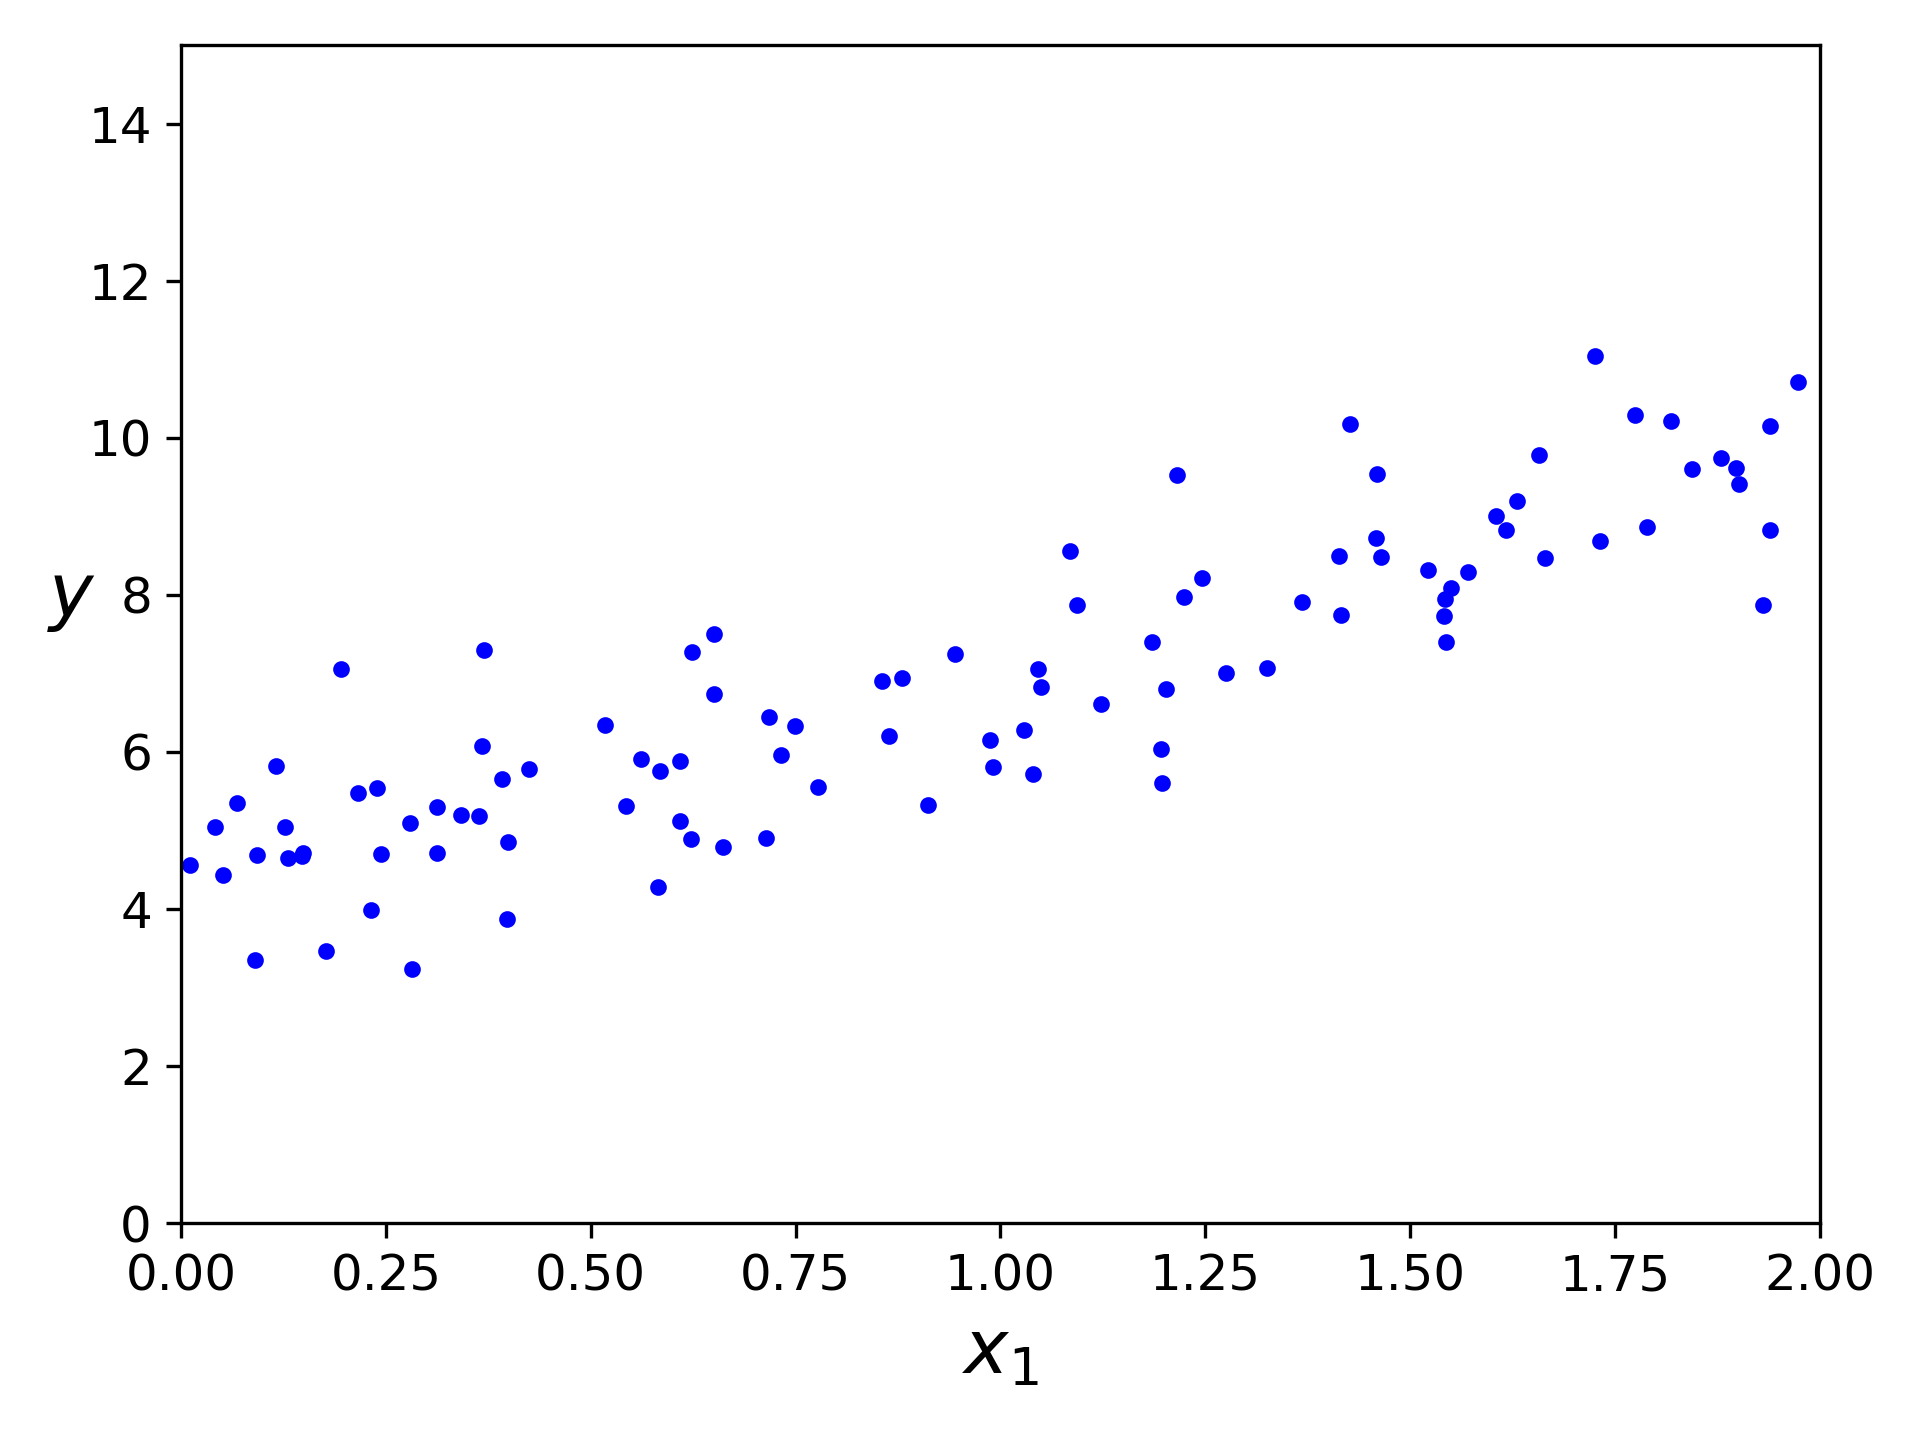
\includegraphics[width=7cm, keepaspectratio]{images/ql_8.png}
			\end{center}
		\end{column}
	\end{columns}
\end{frame}

\begin{frame}{Függvény illesztés alapjai}
	\begin{columns}
		\begin{column}{.5\textwidth}
			Az illesztett modell alakját és viselkedését a \textbf{paraméterei} határozzák meg, amelyek együtthatókként viselkednek a modell egyenletében. A lineáris modell egyenlete: 
			\begin{block}{}
				\vspace{-0.25cm}
				\[
				y_i = \theta_0 + \theta_1x_i + \varepsilon_i
				\]
			\end{block}
			Ahol:
			\begin{itemize}
				\item $\theta_0$: az $y$ tengely metszéspontja, vagy eltolás
				\item $\theta_1$: az egyenes meredeksége
				\item $\varepsilon$: a véletlen hiba, amit a modell nem tud előre jelezni
			\end{itemize}
			$\theta=[\theta_0,\theta_1,...,\theta_n]$ a paraméterek vektora.
		\end{column}
		\begin{column}{.5\textwidth}
			\begin{center}
				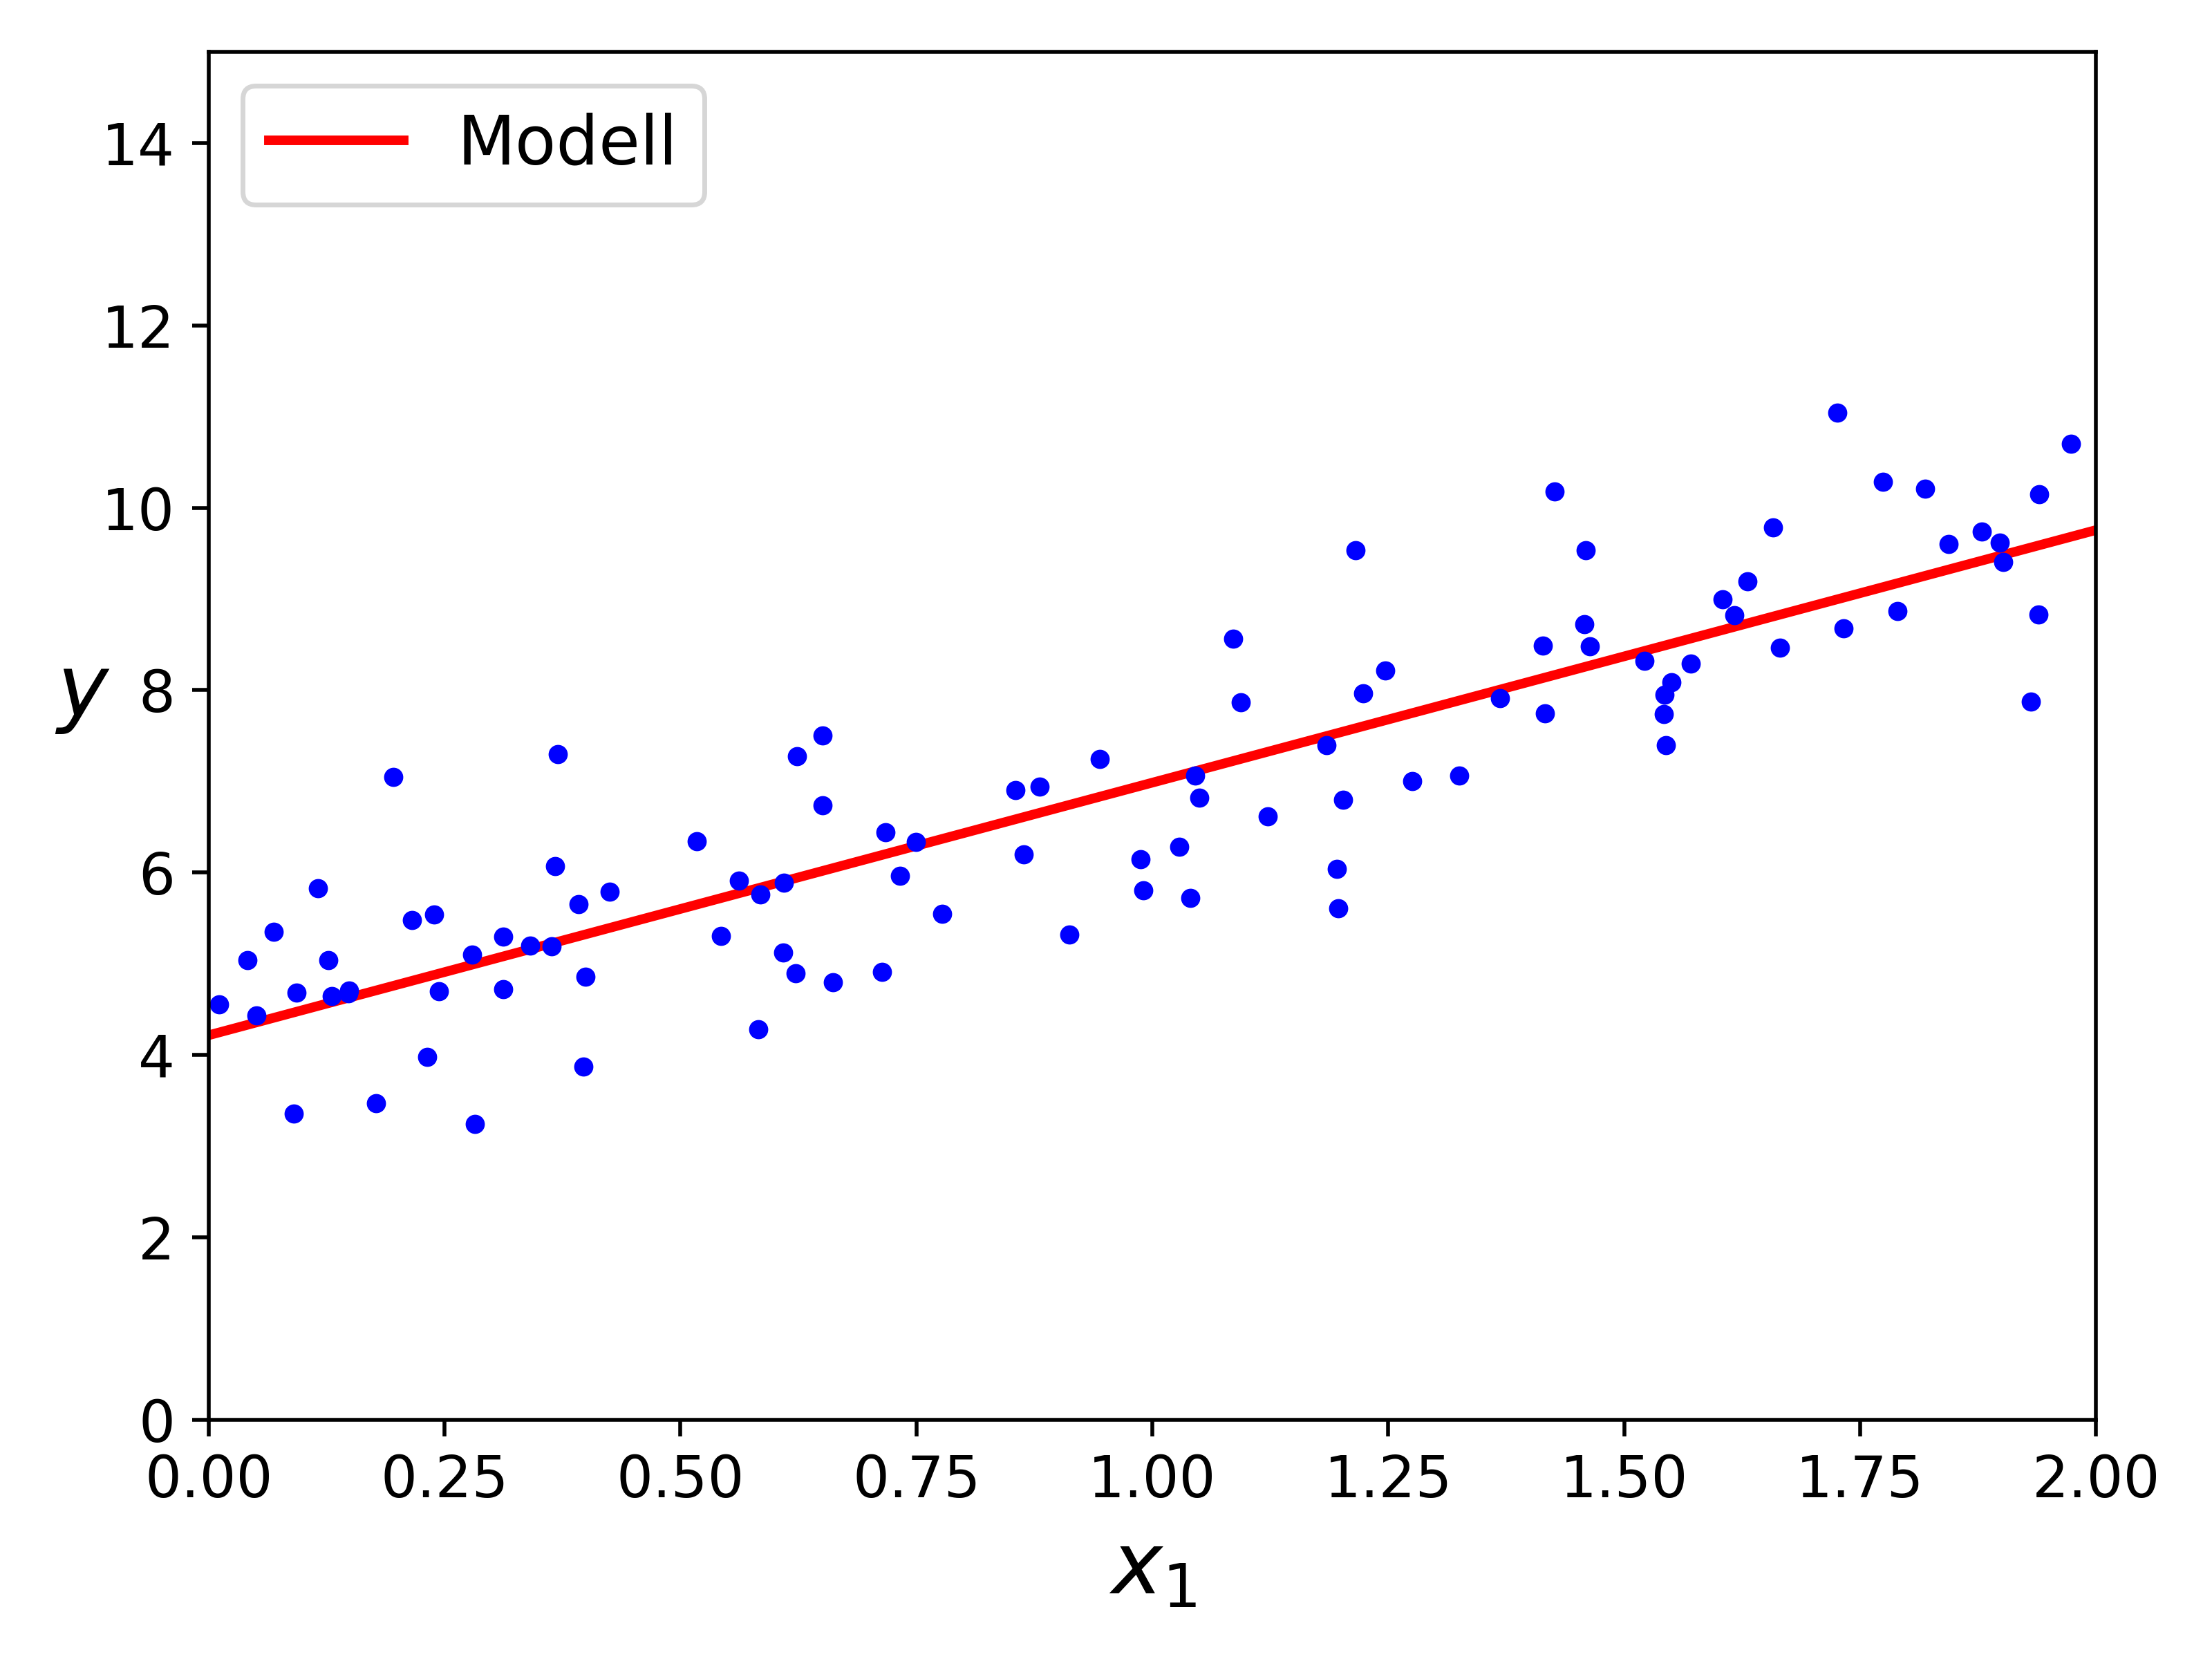
\includegraphics[width=7cm, keepaspectratio]{images/ql_9.png}
			\end{center}
		\end{column}
	\end{columns}
\end{frame}

\begin{frame}{Függvény illesztés több paraméterrel}
	\begin{columns}
		\begin{column}{.5\textwidth}
			Függvényt lehetséges nemlineáris adatokra is illeszteni. Ebben a példában a minta adatpontok kvadratikusak, \textbf{nem írhatók le egy lineáris egyenlettel}. A modellnek ebben az esetben $3$ paramétere van: $\theta_0$, $\theta_1$ és $\theta_2$. Az illesztett modell egyenlete: 
			\[
			y=1.78 + 0.93x + 0.56 x^2
			\]
			Tehát ebben az esetben $\theta_0=1.78$, $\theta_1=0.93$ és $\theta_2=0.56$.
		\end{column}
		\begin{column}{.5\textwidth}
			\begin{center}
				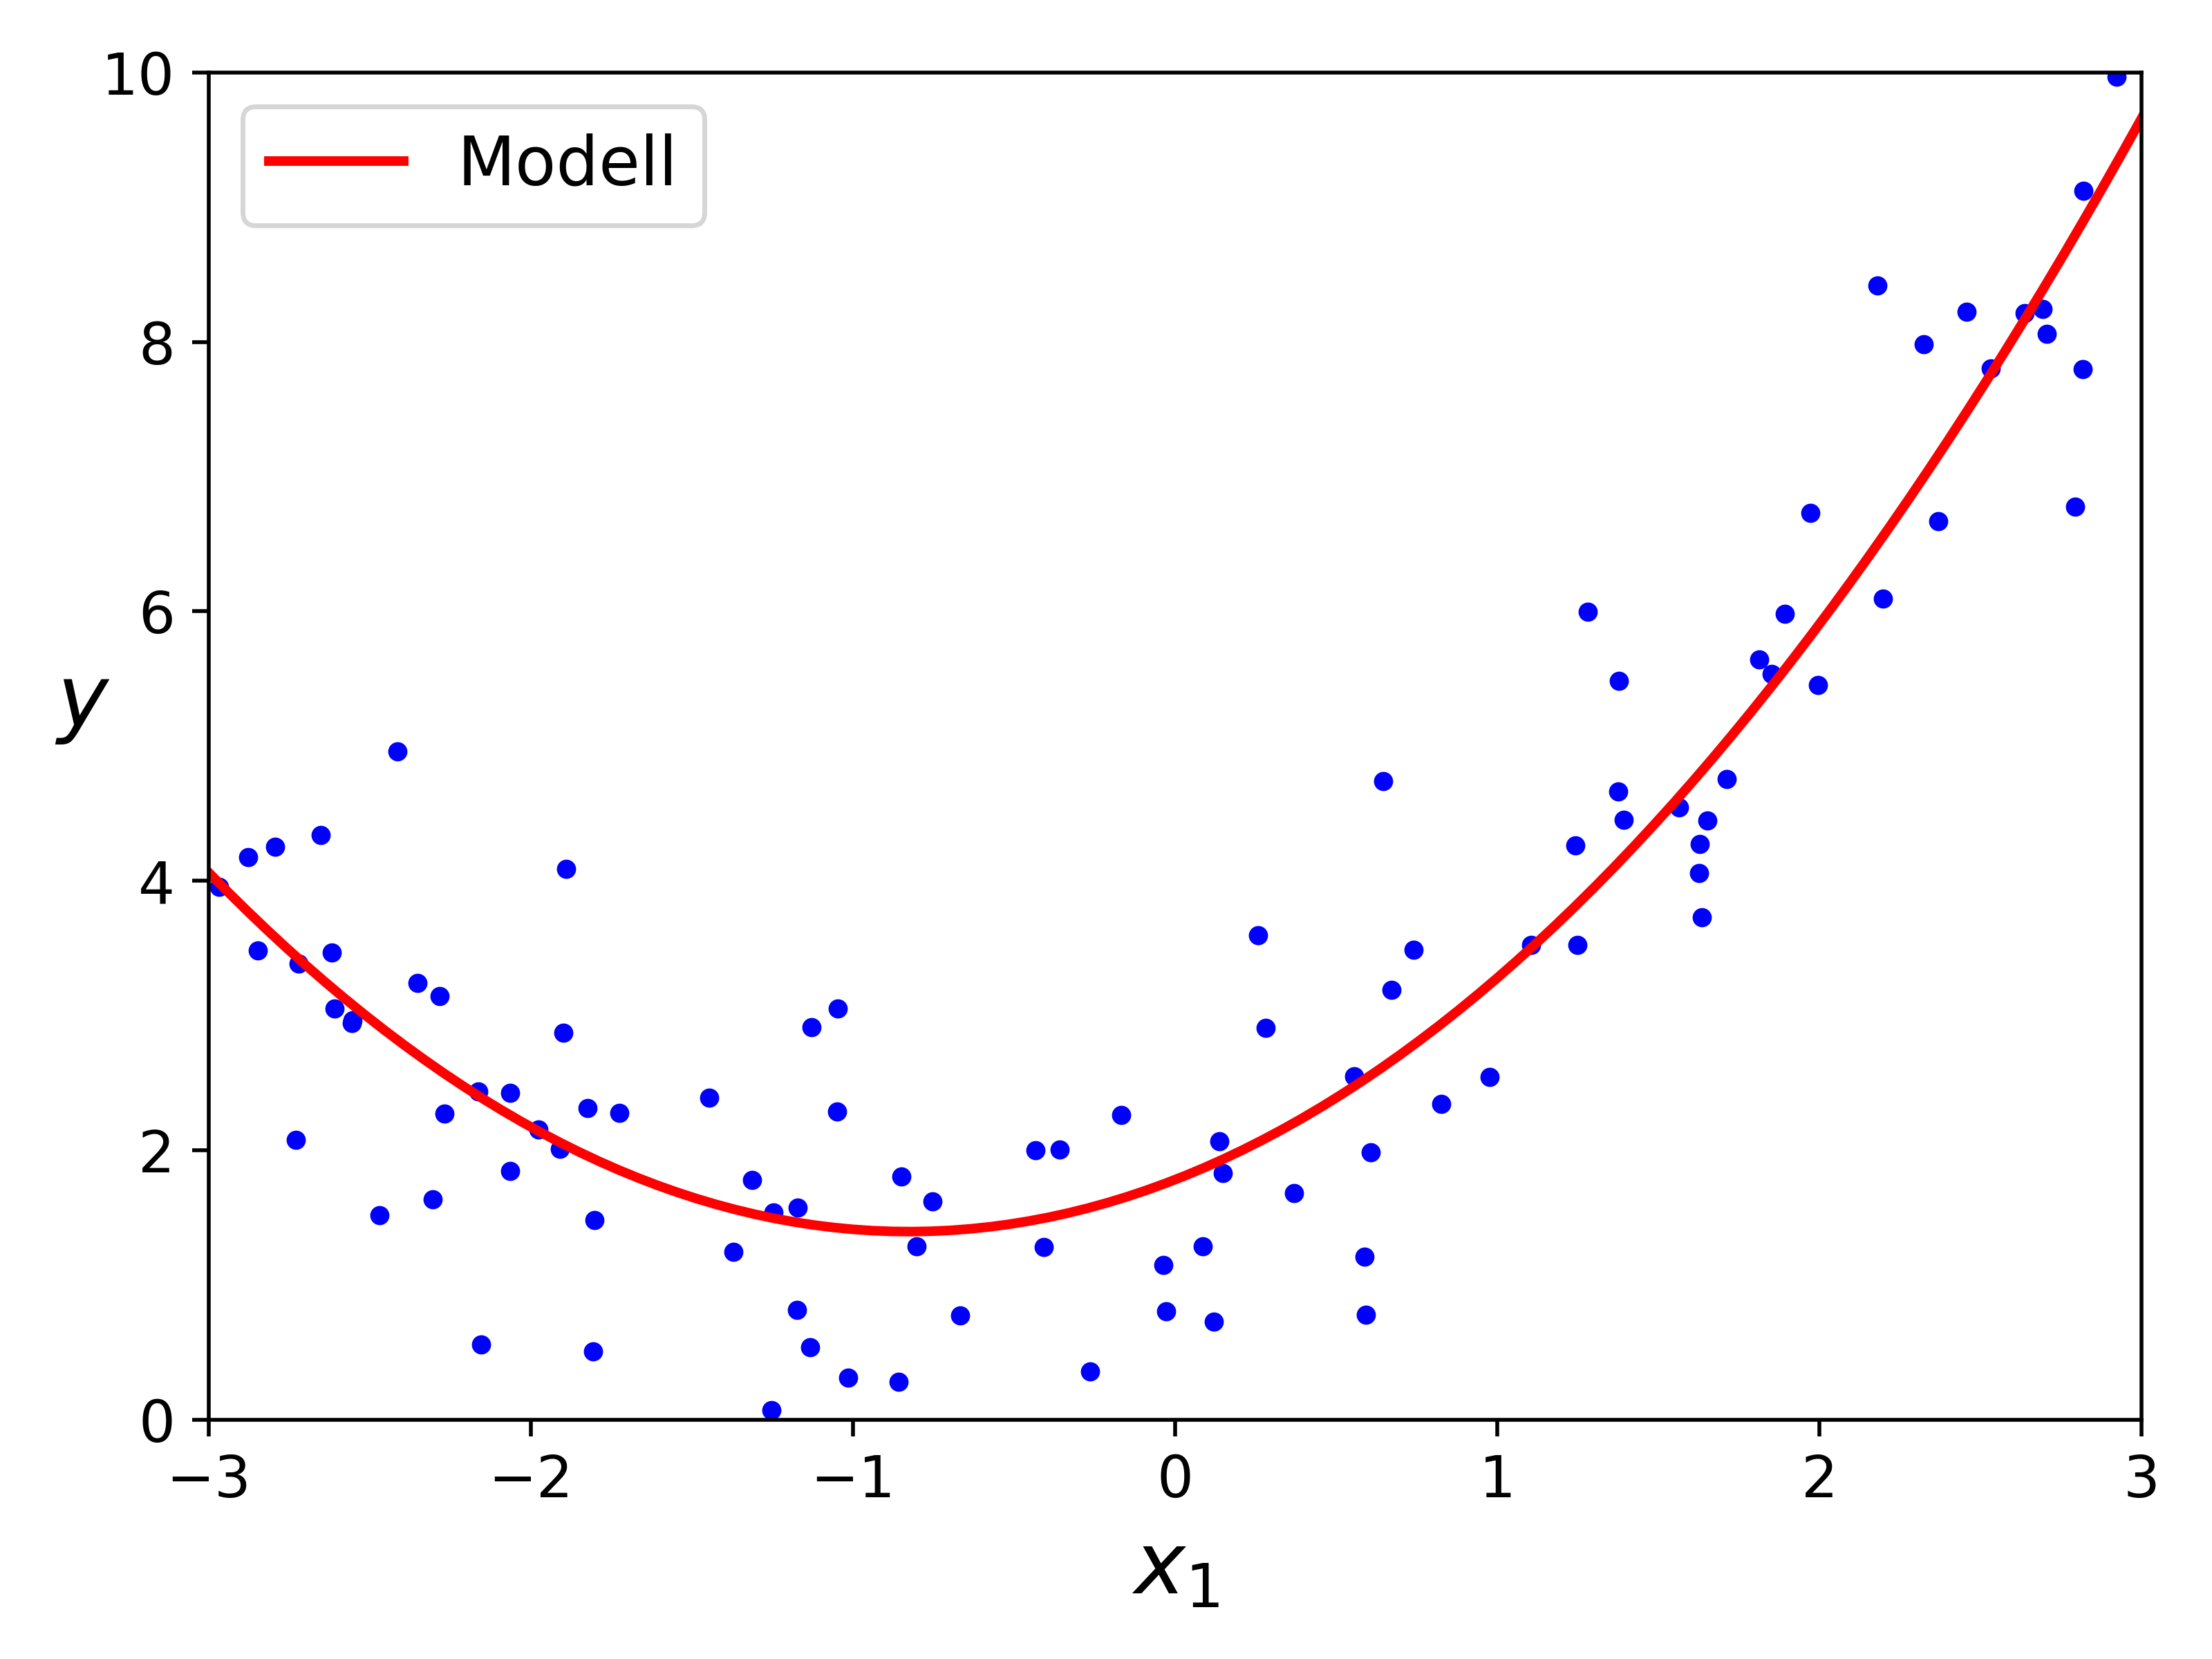
\includegraphics[width=7cm, keepaspectratio]{images/ql_10.png}
			\end{center}
		\end{column}
	\end{columns}
\end{frame}

\section{Gradiens ereszkedés}

\begin{frame}
	\tableofcontents[currentsection]
\end{frame}

\begin{frame}{A költségfüggvény}
	\begin{columns}
		\begin{column}{.5\textwidth}
			A modell illesztő algoritmusok mindegyike úgy találja meg az optimális függvényt, hogy valamilyen költségfüggvényt minimalizál. A leggyakoribb ilyen költségfüggvény az \textbf{átlagos négyzetes hiba}:
			\begin{block}{}
				\[
				MSE = \frac{1}{n} \sum_{i=1}^n \left( y_i - f(x)_i \right)^2
				\]
				\begin{itemize}
					\item $y_i$: Megfigyelt adatpont
					\item $f(x)_i$: Modell által adott becslés
				\end{itemize}
			\end{block}
		\end{column}
		\begin{column}{.5\textwidth}
			\begin{center}
				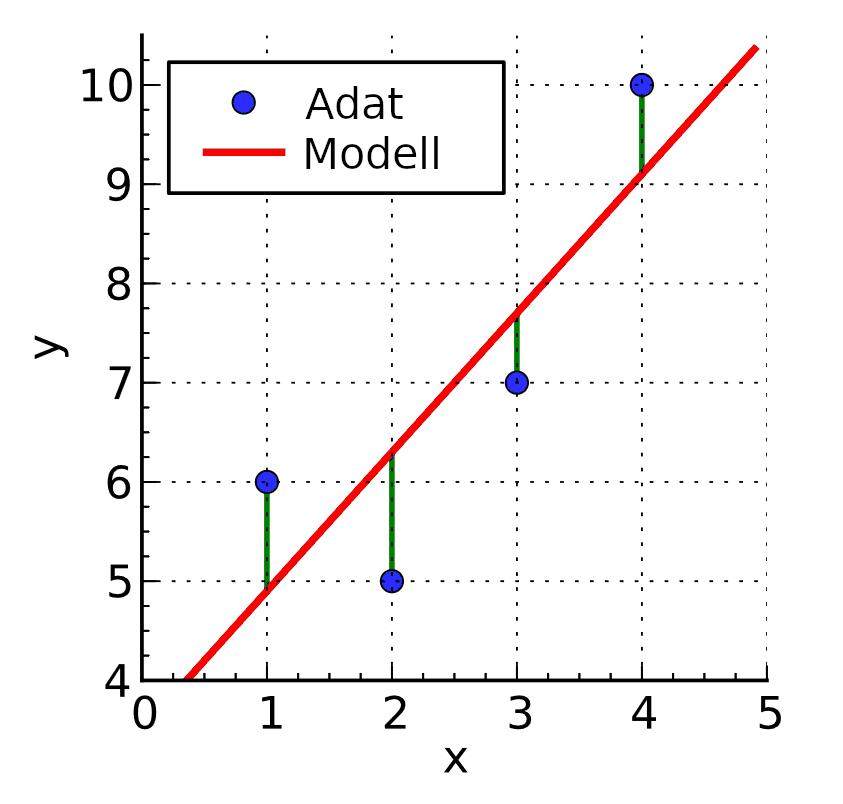
\includegraphics[width=6cm, keepaspectratio]{images/ql_11.png}
			\end{center}
		\end{column}
	\end{columns}
\end{frame}

\begin{frame}{A gradiens}
	\begin{columns}
		\begin{column}{.5\textwidth}
			A függvény illesztés célja, hogy megtalálja azt a modellt, ami a legjobban illeszkedik az adatpontokra, tehát \textbf{minimalizálja a költségfüggvényt} (MSE). 
			\begin{block}{Gradiens}
				Olyan vektor, amely megmutatja hogyan változik a függvény, és megadja a legnagyobb változás irányát minden dimenzióban.
				\vspace{-0.25cm}
				\[
				df = \nabla f * dx
				\]
			\end{block} 
			A gradiens segítségével meg lehet határozni, merre és mennyivel érdemes változtatni a paramétereket a célfüggvény értékének csökkentése érdekében.
		\end{column}
		\begin{column}{.5\textwidth}
			\begin{center}
				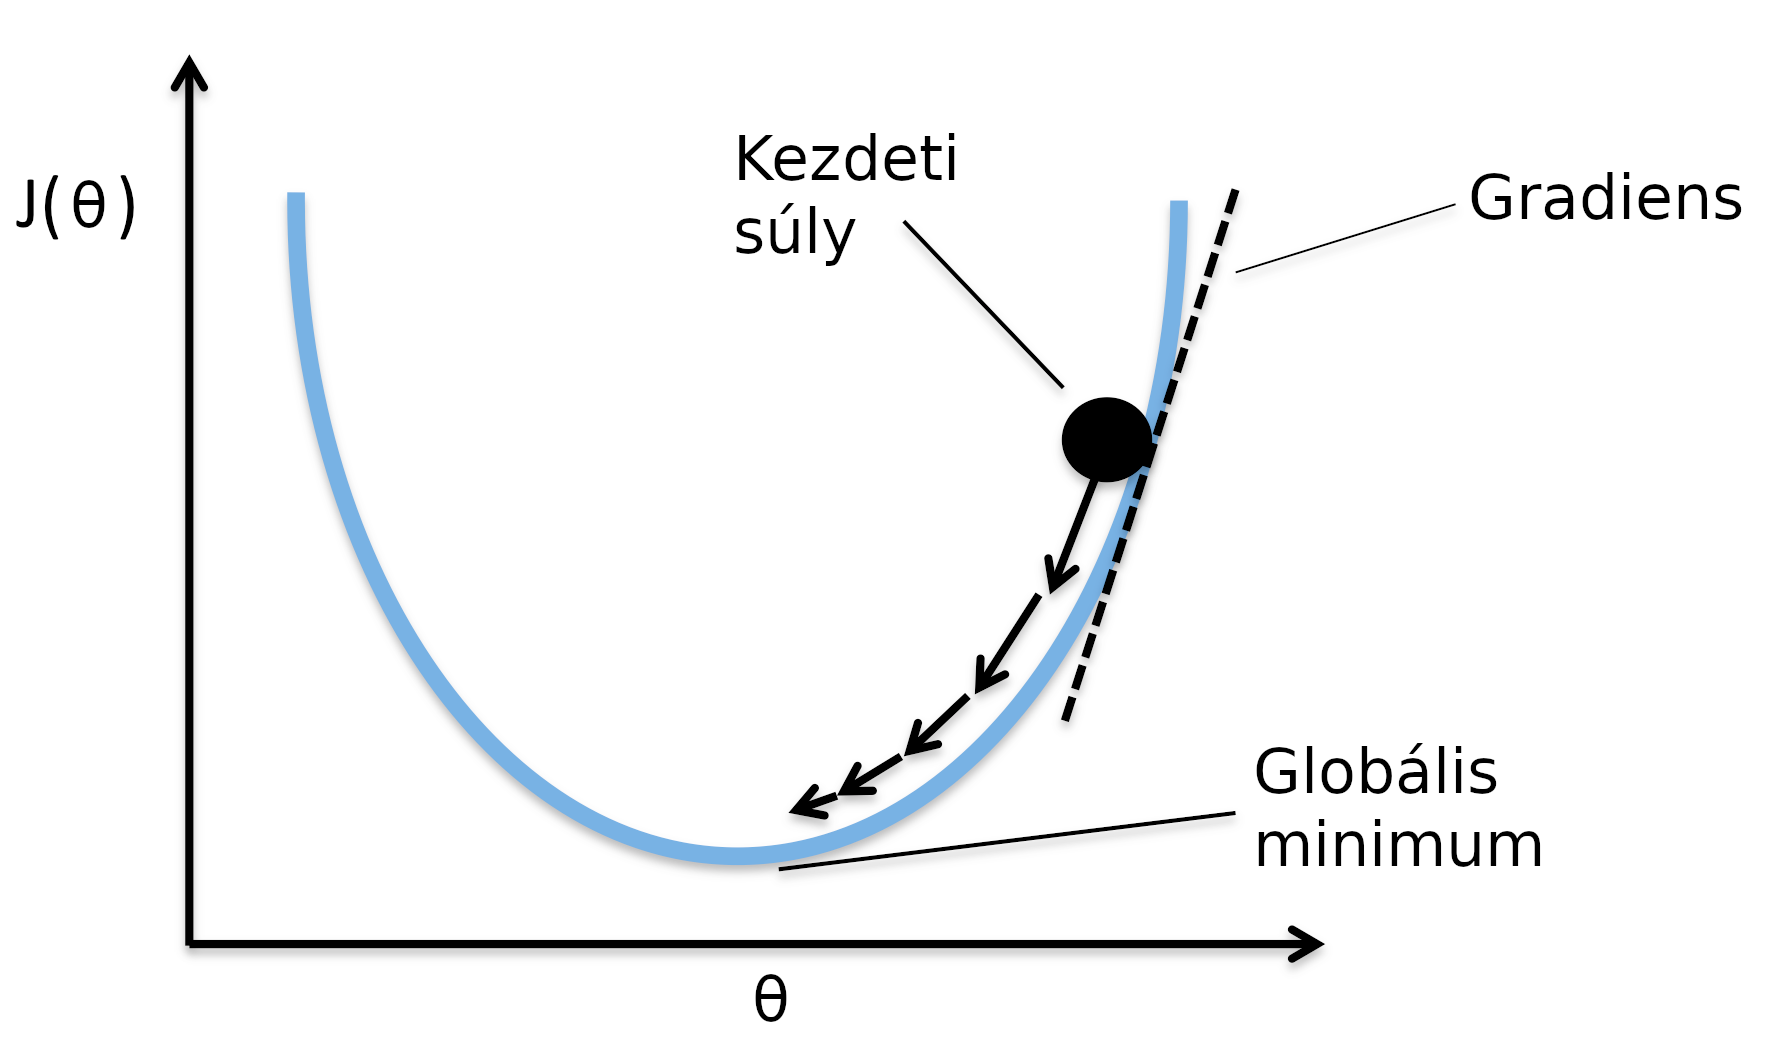
\includegraphics[width=7.5cm, keepaspectratio]{images/ql_12.png}
			\end{center}
		\end{column}
	\end{columns}
\end{frame}

\begin{frame}{Gradiens ereszkedés}
	\begin{columns}
		\begin{column}{.5\textwidth}
			\only<1>{A gradiens ereszkedés egy iteratív minimalizálási algoritmus egy tetszőleges függvény lokális minimum helyének megtalálására. Az algoritmus lépésről lépésre mozog a függvény értékének csökkentése érdekében. \par\smallskip
				\begin{block}{Tanulási sebesség ($\alpha$ vagy $\eta$)}
					A tanulási sebesség meghatározza, mennyire nagy lépéseket tesz a gradiens ereszkedés az optimalizációs folyamat során.
			\end{block}}
			\only<2>{\begin{block}{A gradiens ereszkedés paraméter frissítése:}
					\[
					\theta' \leftarrow \theta - \alpha \; \nabla_\theta \; J(\theta)
					\]
					\begin{itemize}
						\item $\theta=[\theta_0,\theta_1,...,\theta_n]$: Paraméterek vektora
						\item $\alpha \in [0,1]$: Tanulási sebesség
						\item $\nabla_\theta$: Költségfüggvény gradiense \\($\theta$ szerinti derivált)
						\item $J(\theta)$: Költségfüggvény $\theta$ szerint \\(pl. MSE)
					\end{itemize}
			\end{block}}
		\end{column}
		\begin{column}{.5\textwidth}
			\only<1>{\begin{center}
					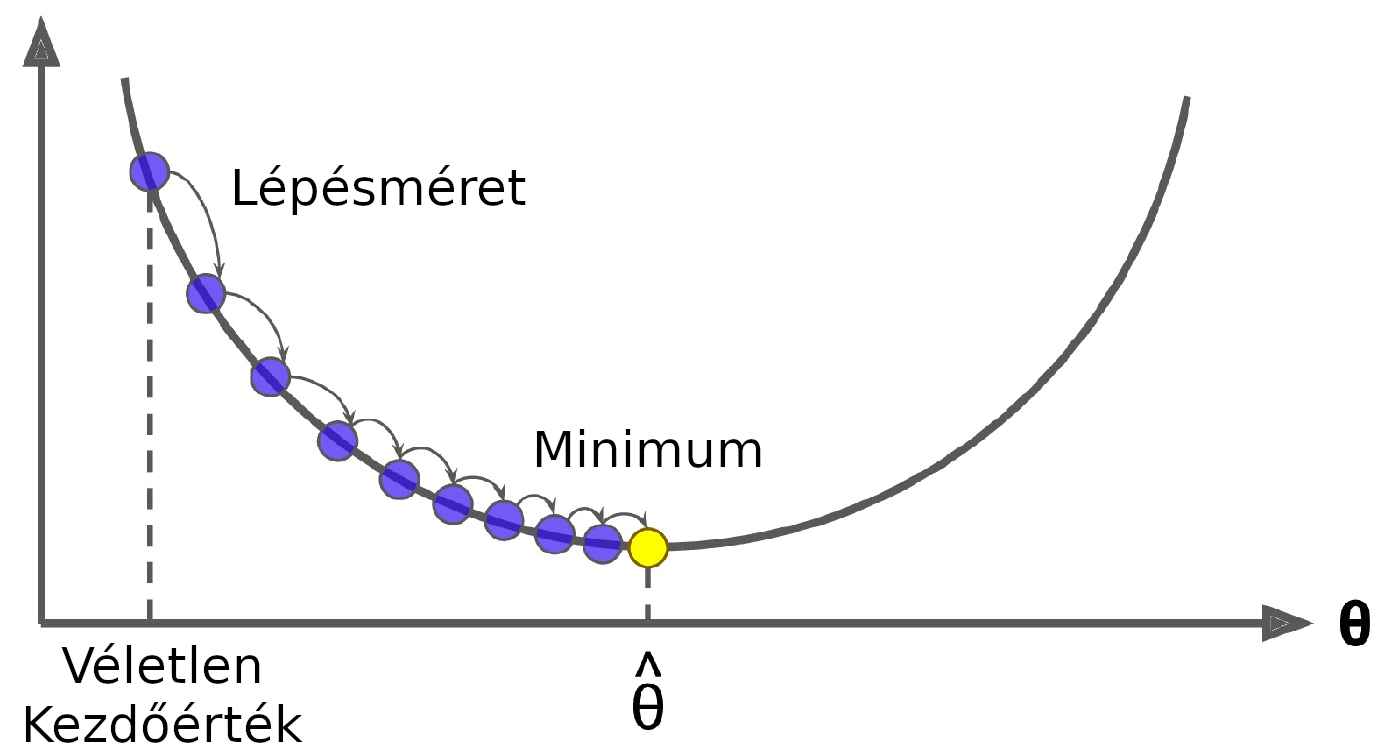
\includegraphics[width=7cm, keepaspectratio]{images/ql_13.png}
			\end{center}}
			\only<2>{\begin{center}
					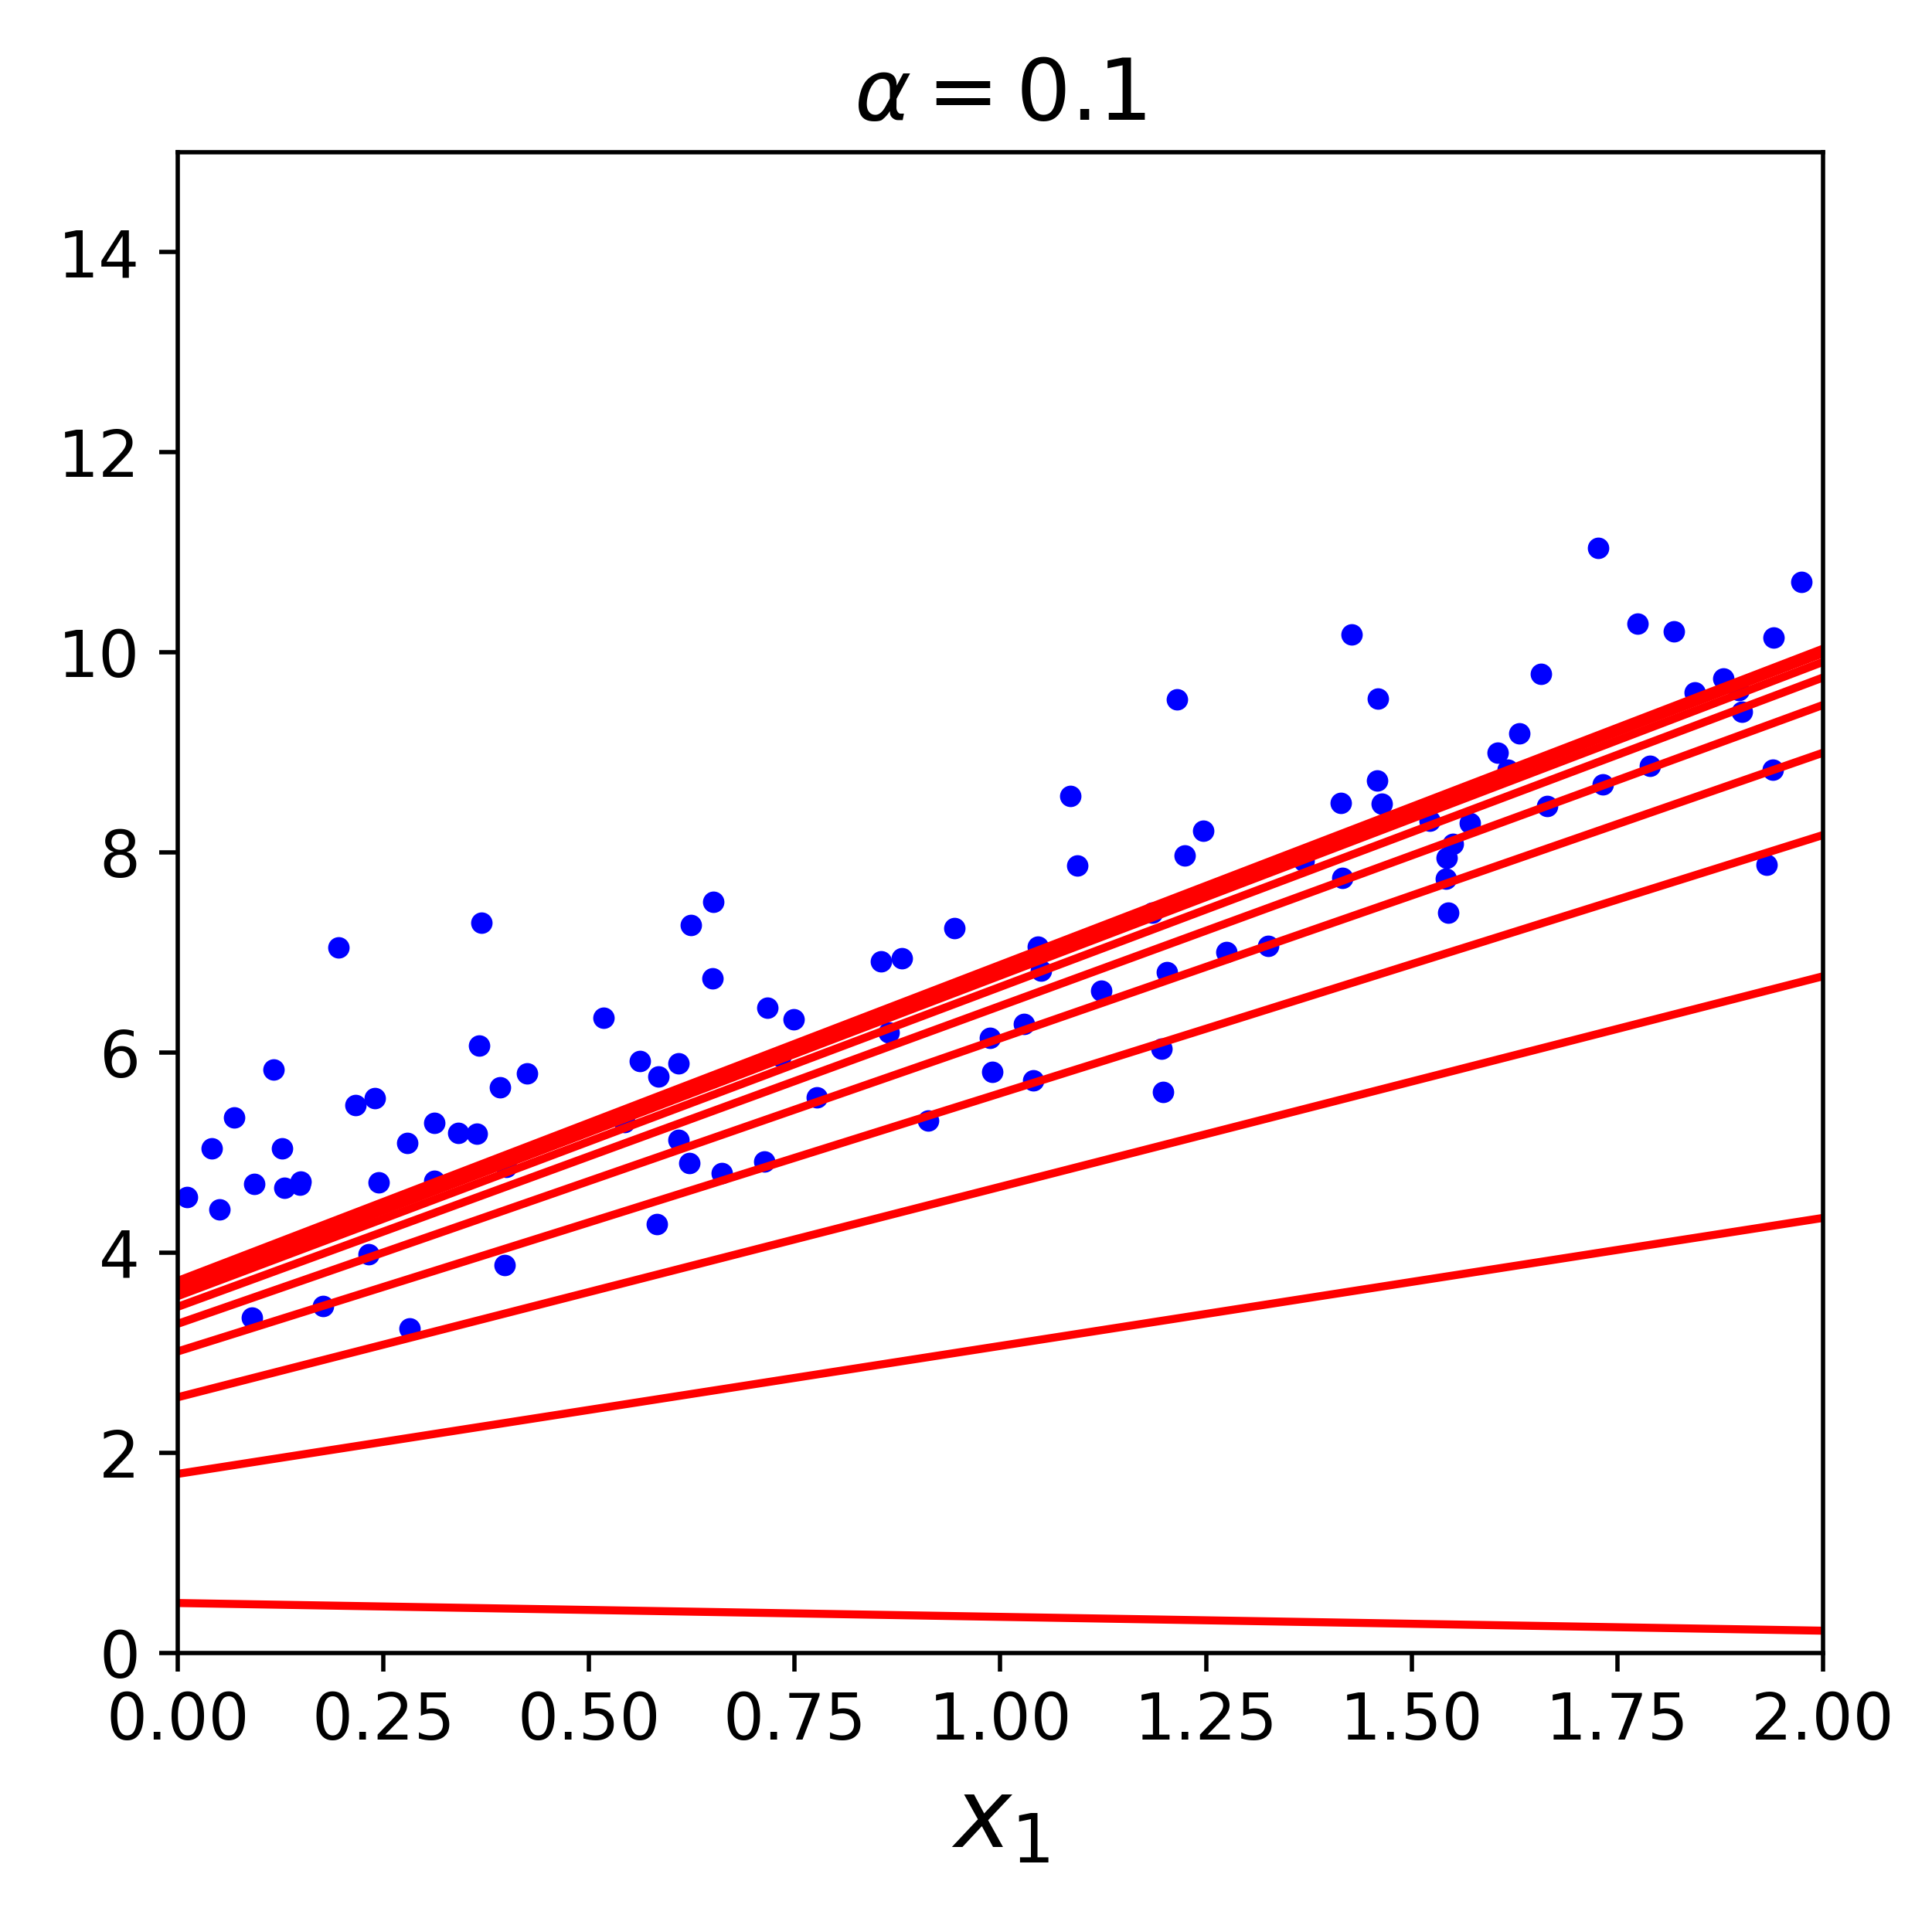
\includegraphics[width=7cm, keepaspectratio]{images/ql_20.png}
			\end{center}}
		\end{column}
	\end{columns}
\begin{flushright}
	
	\end{flushright}\end{frame}

\begin{frame}{Túl alacsony tanulási sebesség}
	\begin{columns}
		\begin{column}{.5\textwidth}
			\begin{center}
				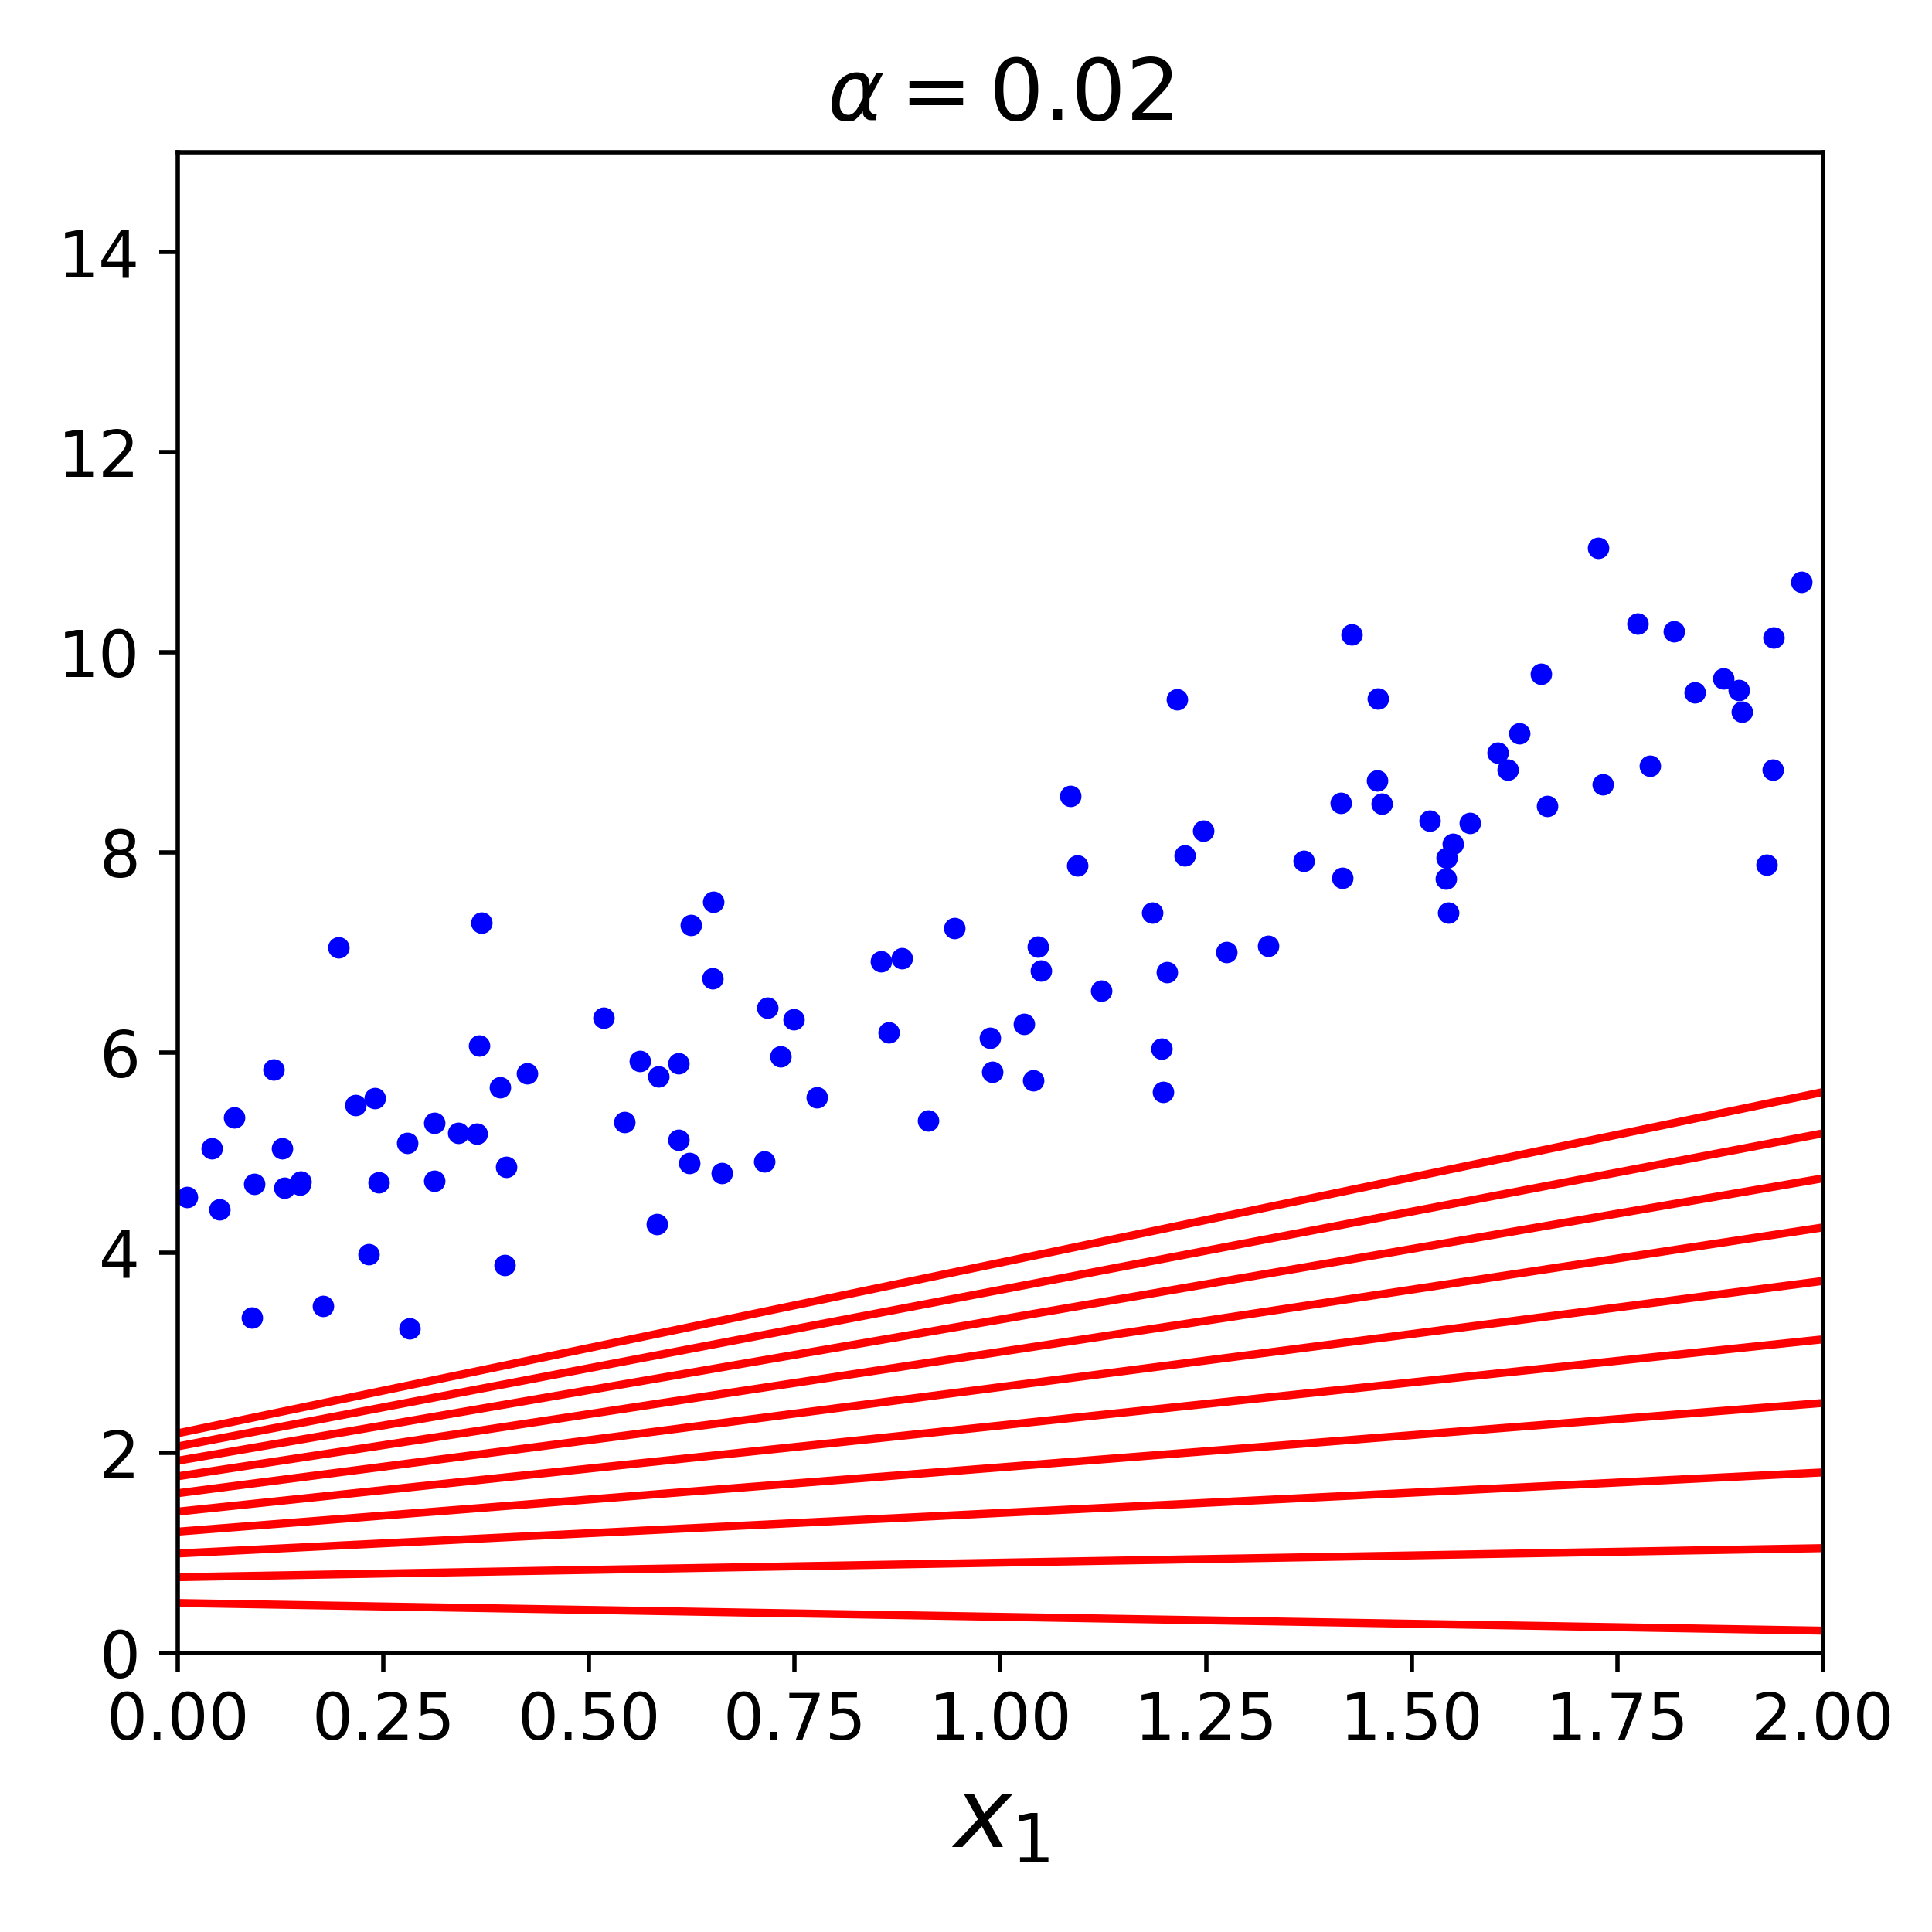
\includegraphics[width=6cm, keepaspectratio]{images/ql_17.png}
			\end{center}
		\end{column}
		\begin{column}{.5\textwidth}
			\begin{center}
				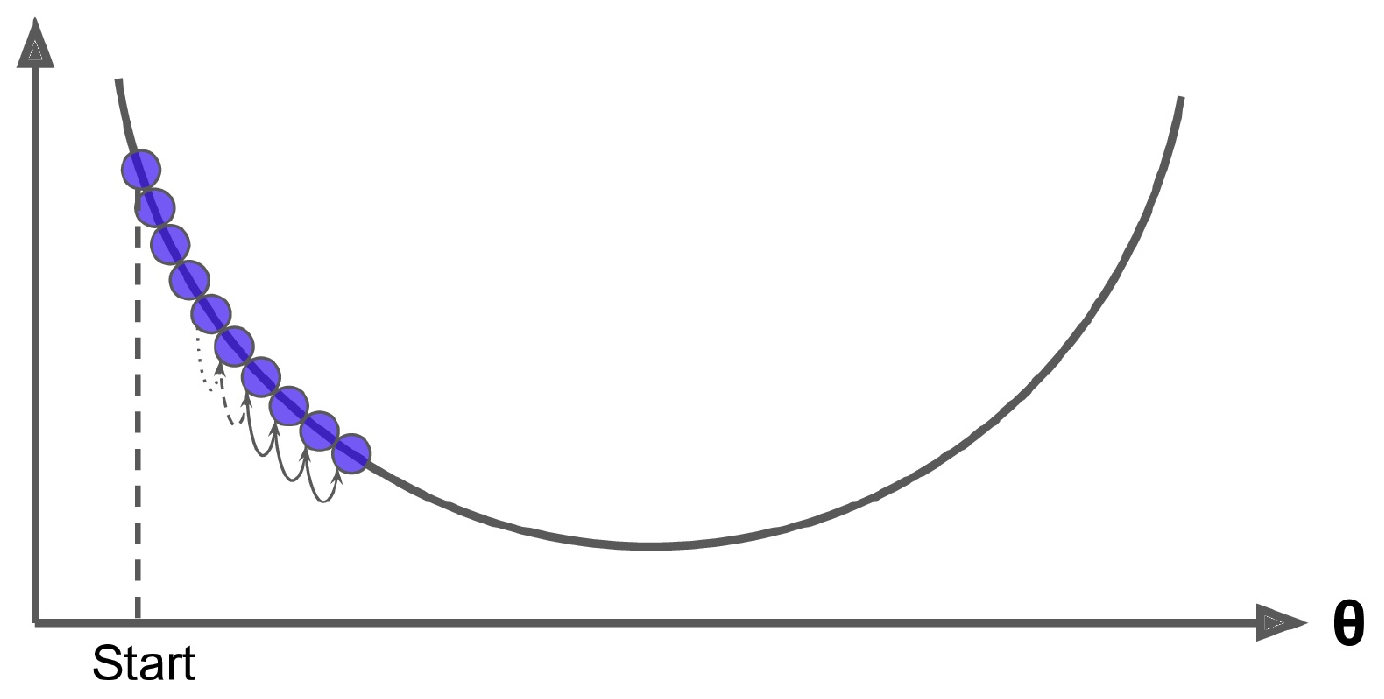
\includegraphics[width=7cm, keepaspectratio]{images/ql_14.png}
			\end{center}
		\end{column}
	\end{columns}
\end{frame}

\begin{frame}{Túl magas tanulási sebesség}
	\begin{columns}
		\begin{column}{.5\textwidth}
			\begin{center}
				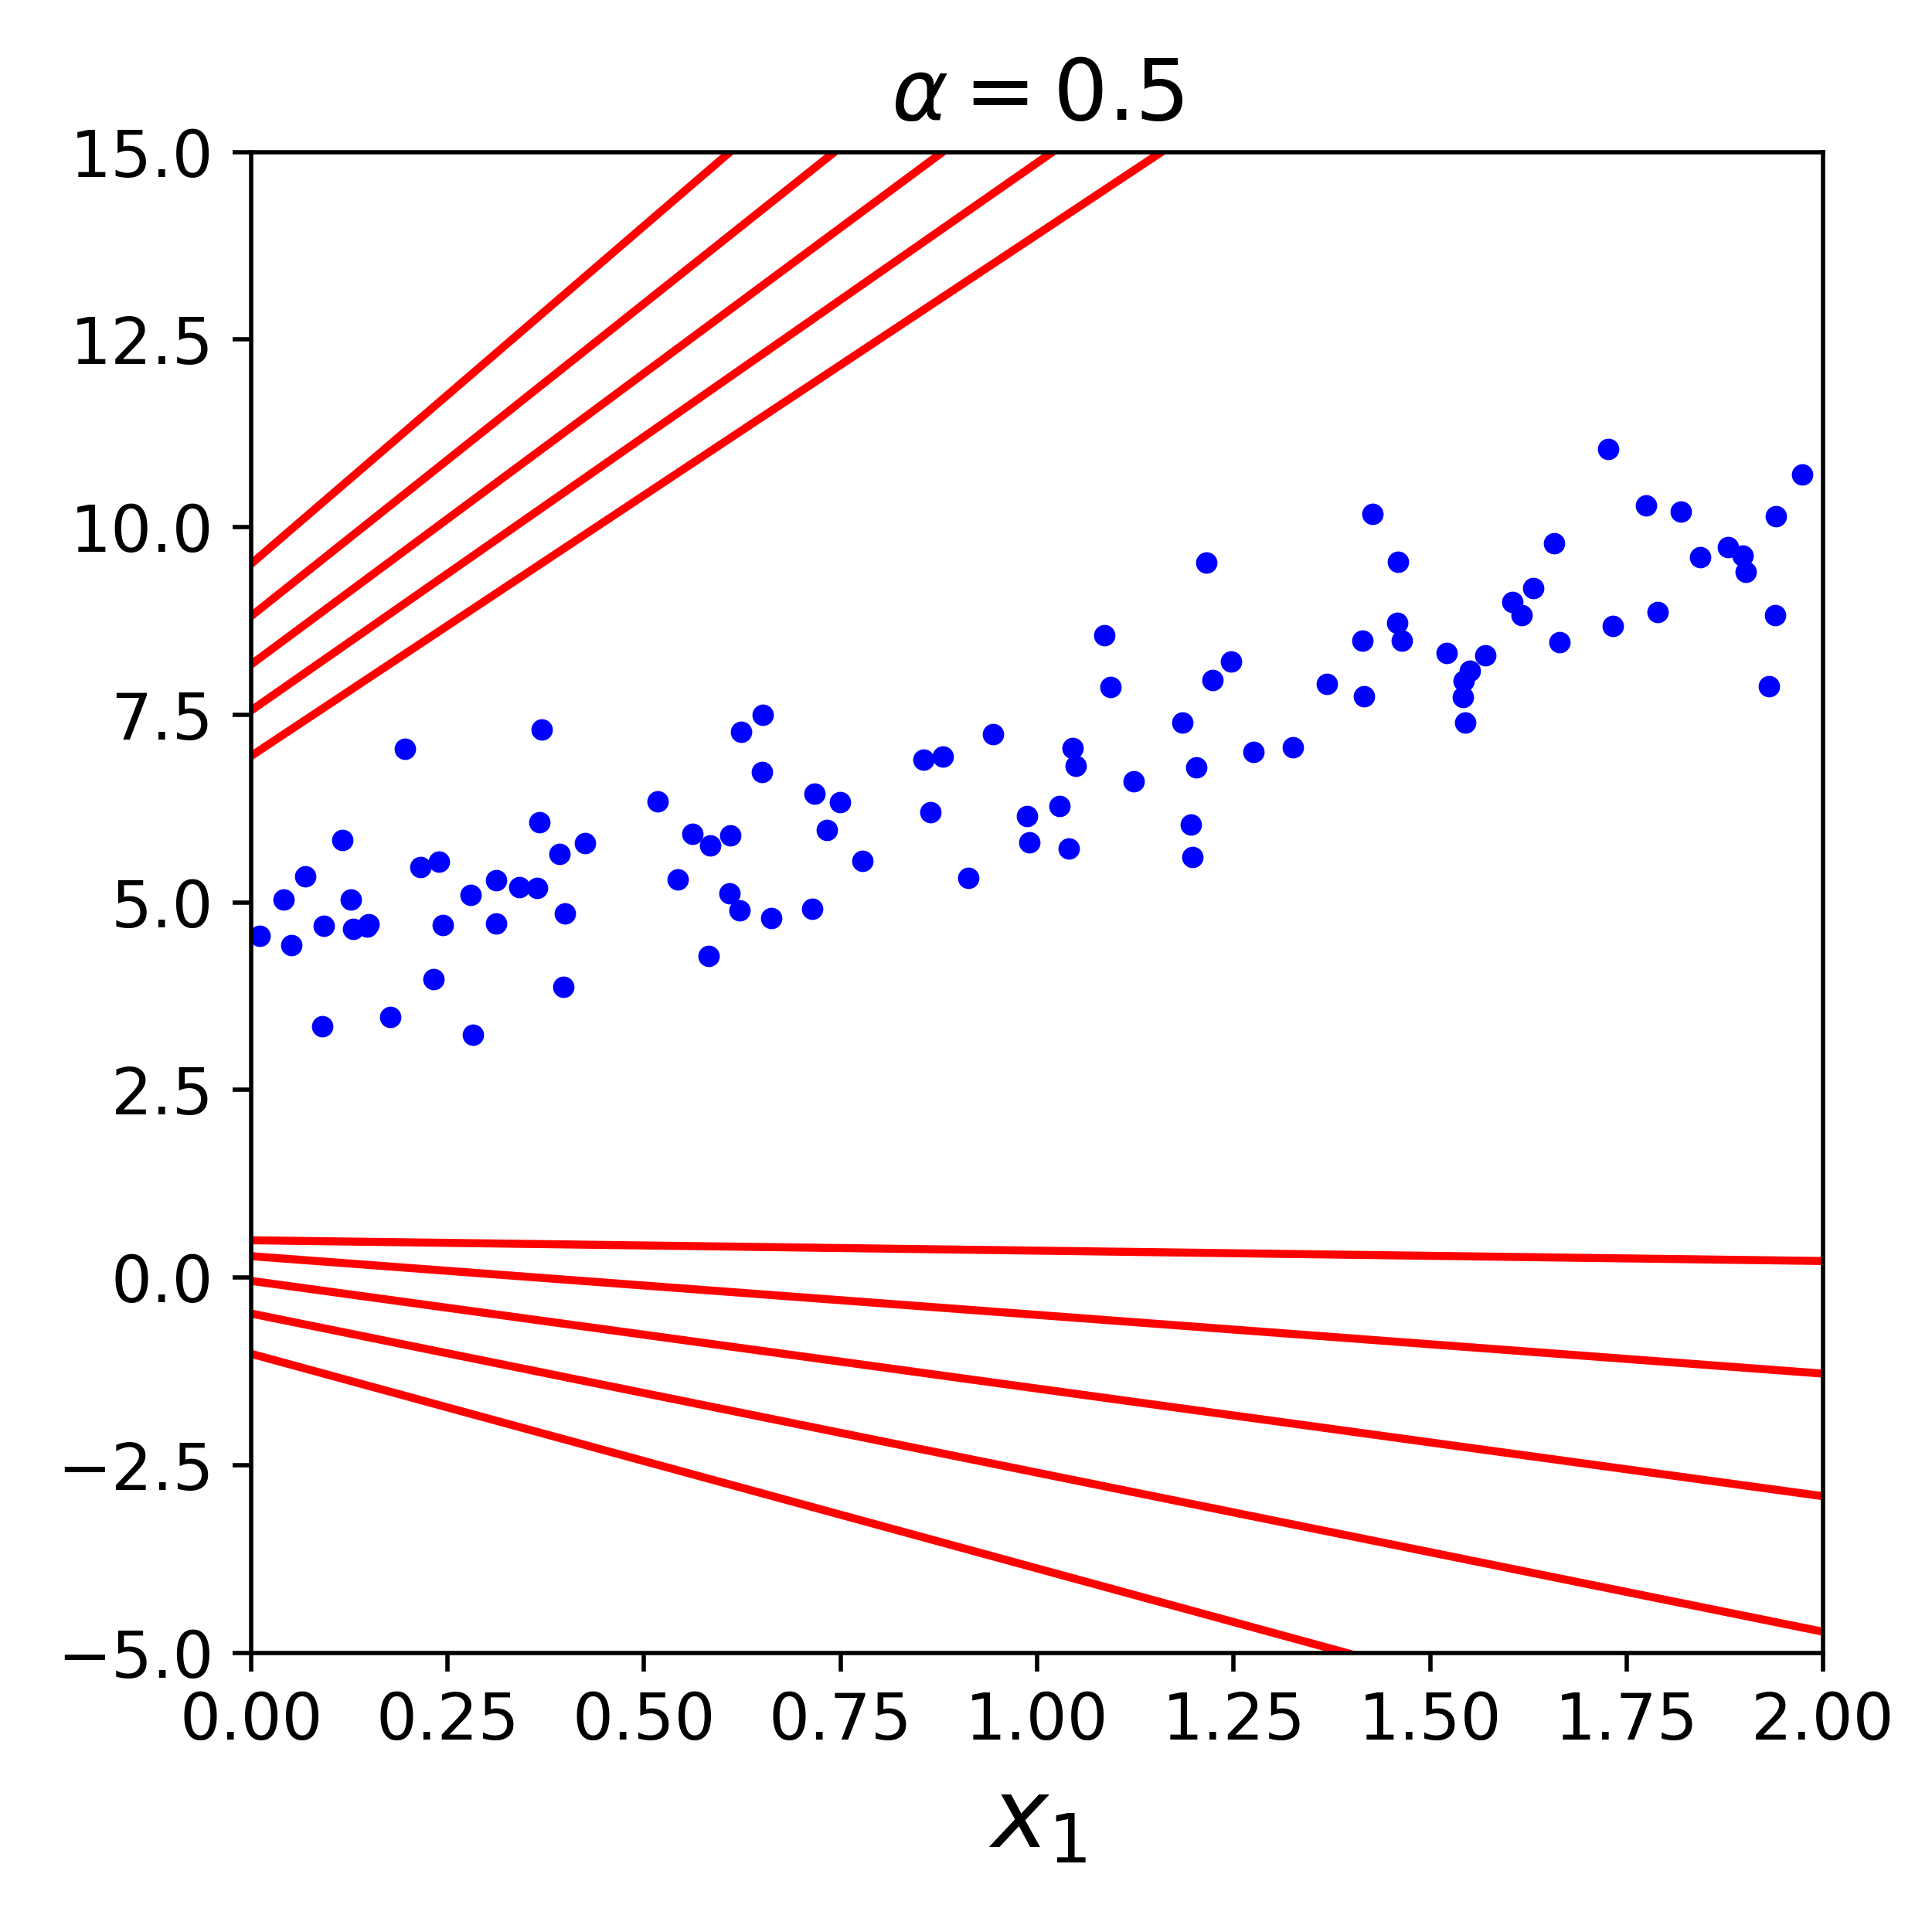
\includegraphics[width=6cm, keepaspectratio]{images/ql_19.png}
			\end{center}
		\end{column}
		\begin{column}{.5\textwidth}
			\begin{center}
				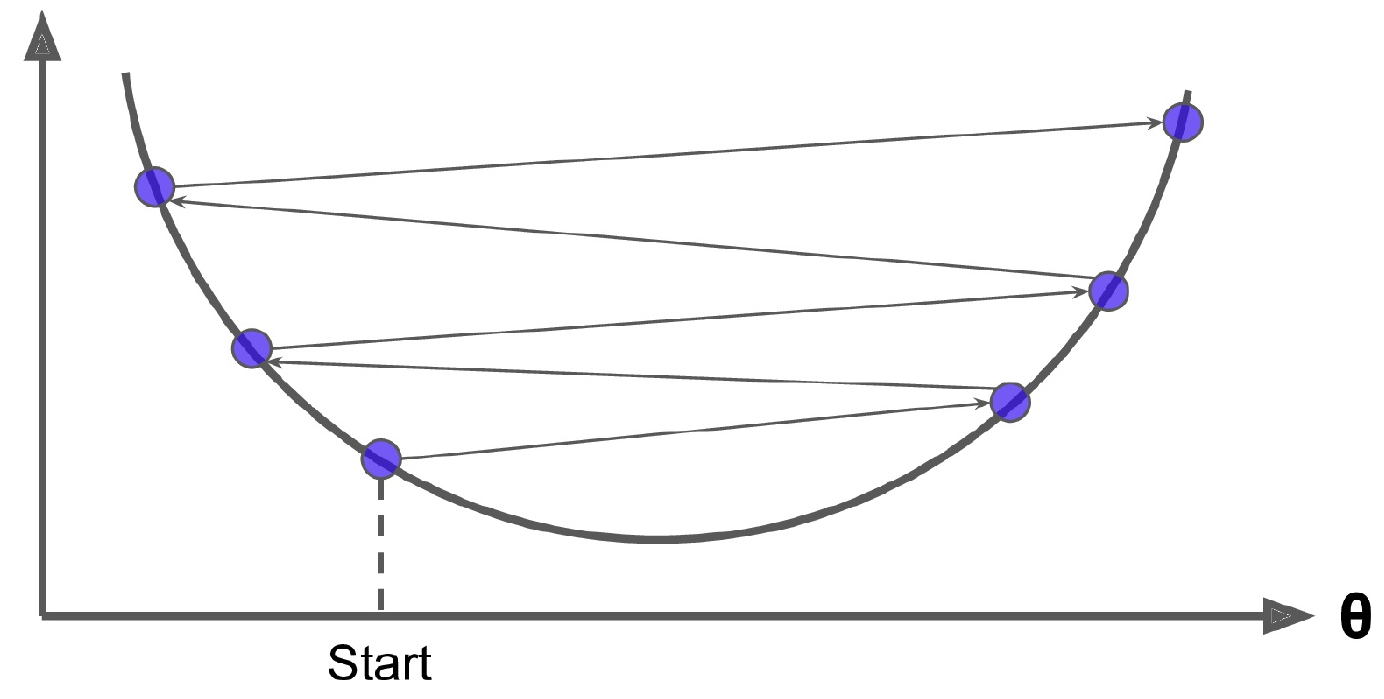
\includegraphics[width=7cm, keepaspectratio]{images/ql_15.png}
			\end{center}
		\end{column}
	\end{columns}
\end{frame}

\begin{frame}{Egyéb problémák}
	\begin{columns}
		\begin{column}{.5\textwidth}
			A gradiens ereszkedés nem garantálja, hogy elér egy globális minimumot, hiszen a gradiens operátora csak lokális változásokat vesz figyelembe. Ebből adódóan az \textbf{algoritmus beragadhat egy lokális minimumon}.\par\medskip
			Vannak esetek, amikor a gradiens nem meghatározható (szaturál), például amikor \textbf{elér egy fennsíkot a függvényen}. Ebben az esetben a futás vagy nagyon lassú lesz, vagy nem halad semerre. 
		\end{column}
		\begin{column}{.5\textwidth}
			\begin{center}
				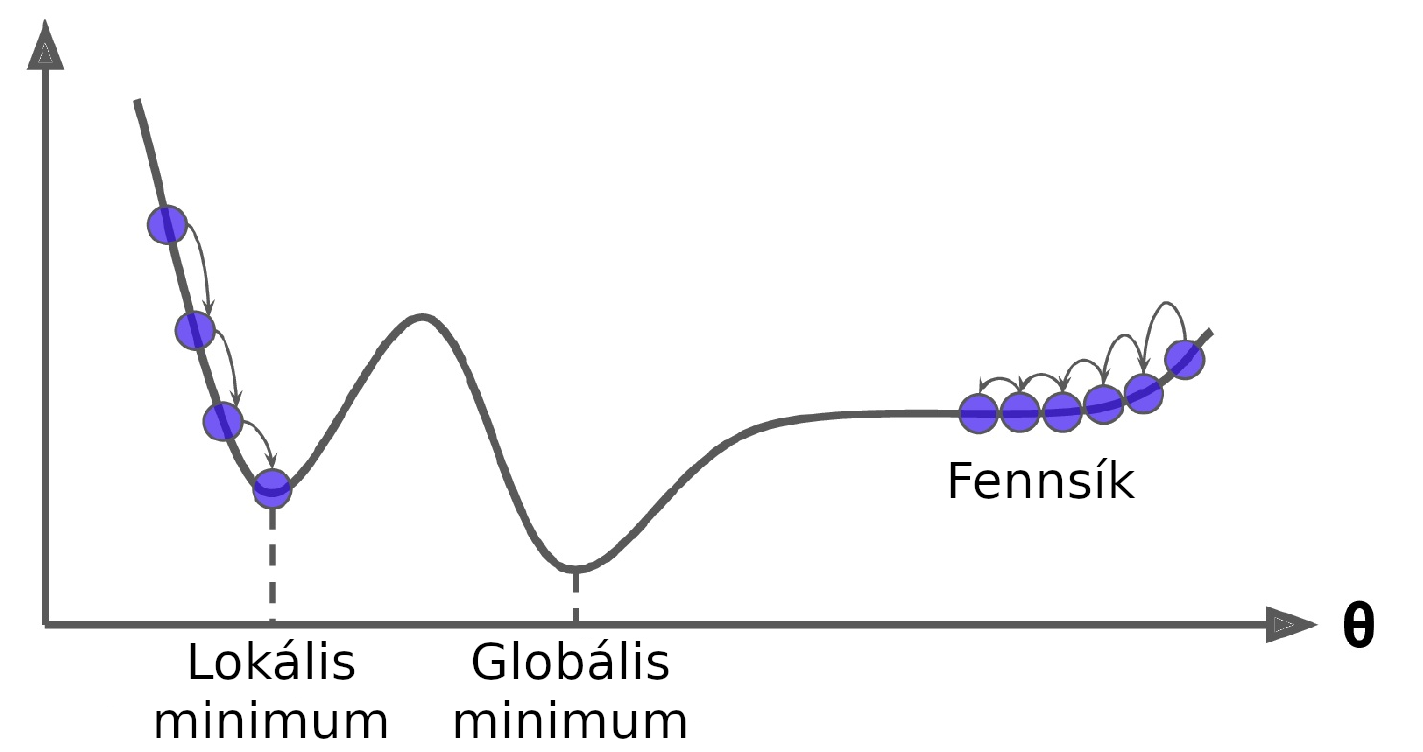
\includegraphics[width=7cm, keepaspectratio]{images/ql_16.png}
			\end{center}
		\end{column}
	\end{columns}
\end{frame}

\section{Neurális hálózatok}

\begin{frame}{}
	\tableofcontents[currentsection]
\end{frame}

\begin{frame}{Biológiai és mesterséges neuronok}
\begin{columns}
\begin{column}{.5\textwidth}
Az ember találmányait mindig a természet ihlette. A repülőgépeket a madarak mintájára, a gépkocsit a lovak inspirálták. A természetes lépés ezután az volt, hogy az emberi agyat is modellezik.\par\medskip
Az első perceptron modellt Warren McCulloh és Walter Pitts hozta létre, először pedig Frank Rosenblatt épített egy perceptron gépet. Ez egy képfelismerő gép volt, 400 véletlenszerűen kapcsolt fotocella volt az érzékelője. A súlyokat potenciométerek implementálták, és a súlyok frissítését elektromotorok hajtották végre. 
\end{column}
\begin{column}{.5\textwidth}
\begin{center}
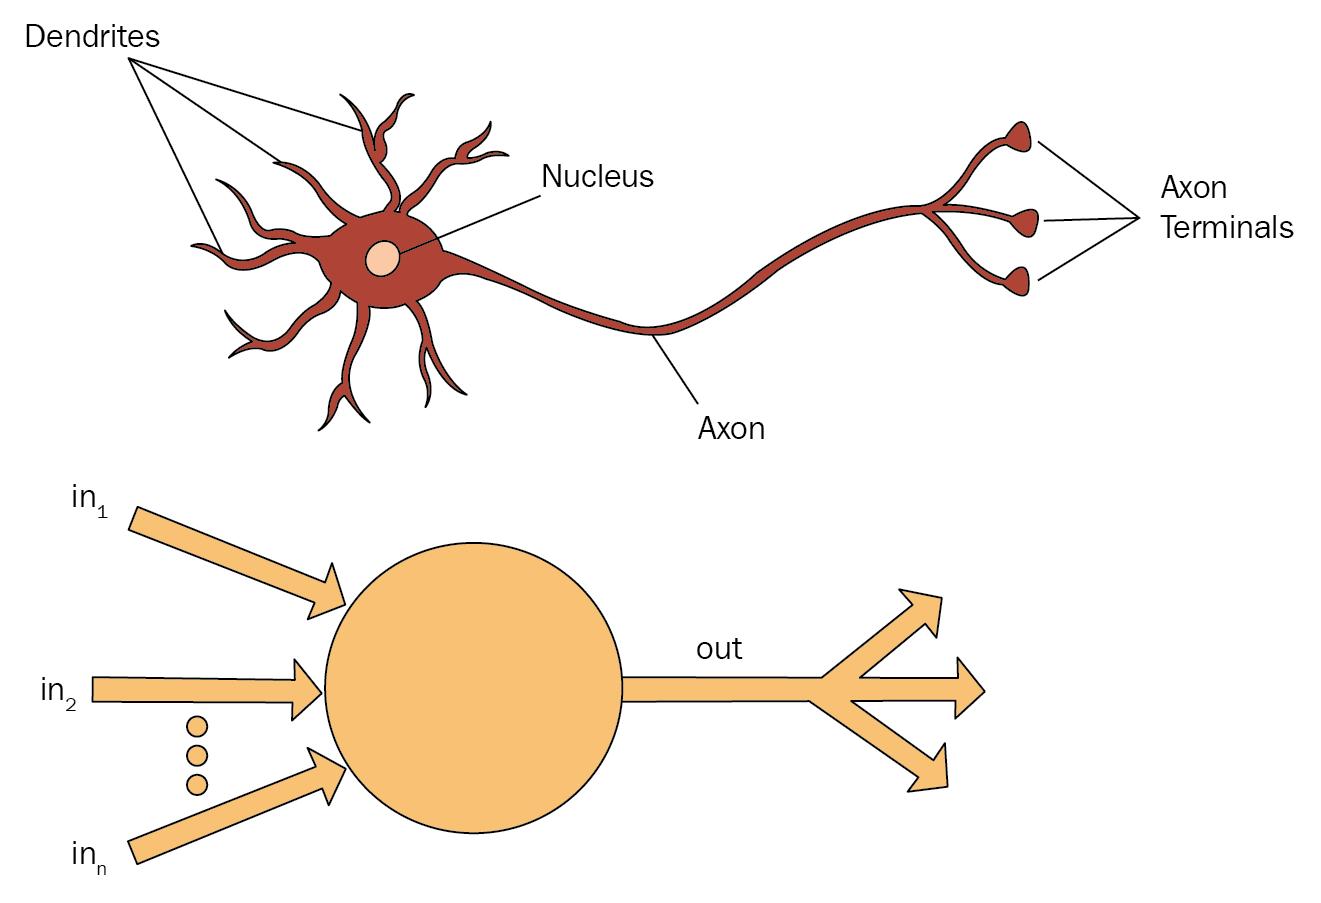
\includegraphics[width=7cm, keepaspectratio]{images/dl_1.png}
\end{center}
\end{column}
\end{columns}
\end{frame}

\begin{frame}{A neuron}
\begin{columns}
\begin{column}{.4\textwidth}
Az egyes neuronok egyszerű elemi műveleteket végeznek. A neuronnak több $x$ inputja (kapcsolata) van, és mindegyikhez egy $w$ \textbf{súly} tartozik.\par\smallskip
A neuron kiszámítja az inputjainak a súlyozott szorzatösszegét:
\begin{block}{}
\vspace{-0.7cm}
\[
z=x_1w_1 + x_2w_2 + ... + x_nw_n
\]
\end{block}
majd ezt az értéket behelyettesíti egy aktivációs függvénybe:
\begin{block}{}
\vspace{-0.2cm}
\[
h=\varphi(z)
\]
\end{block}
\end{column}
\begin{column}{.6\textwidth}
\begin{center}
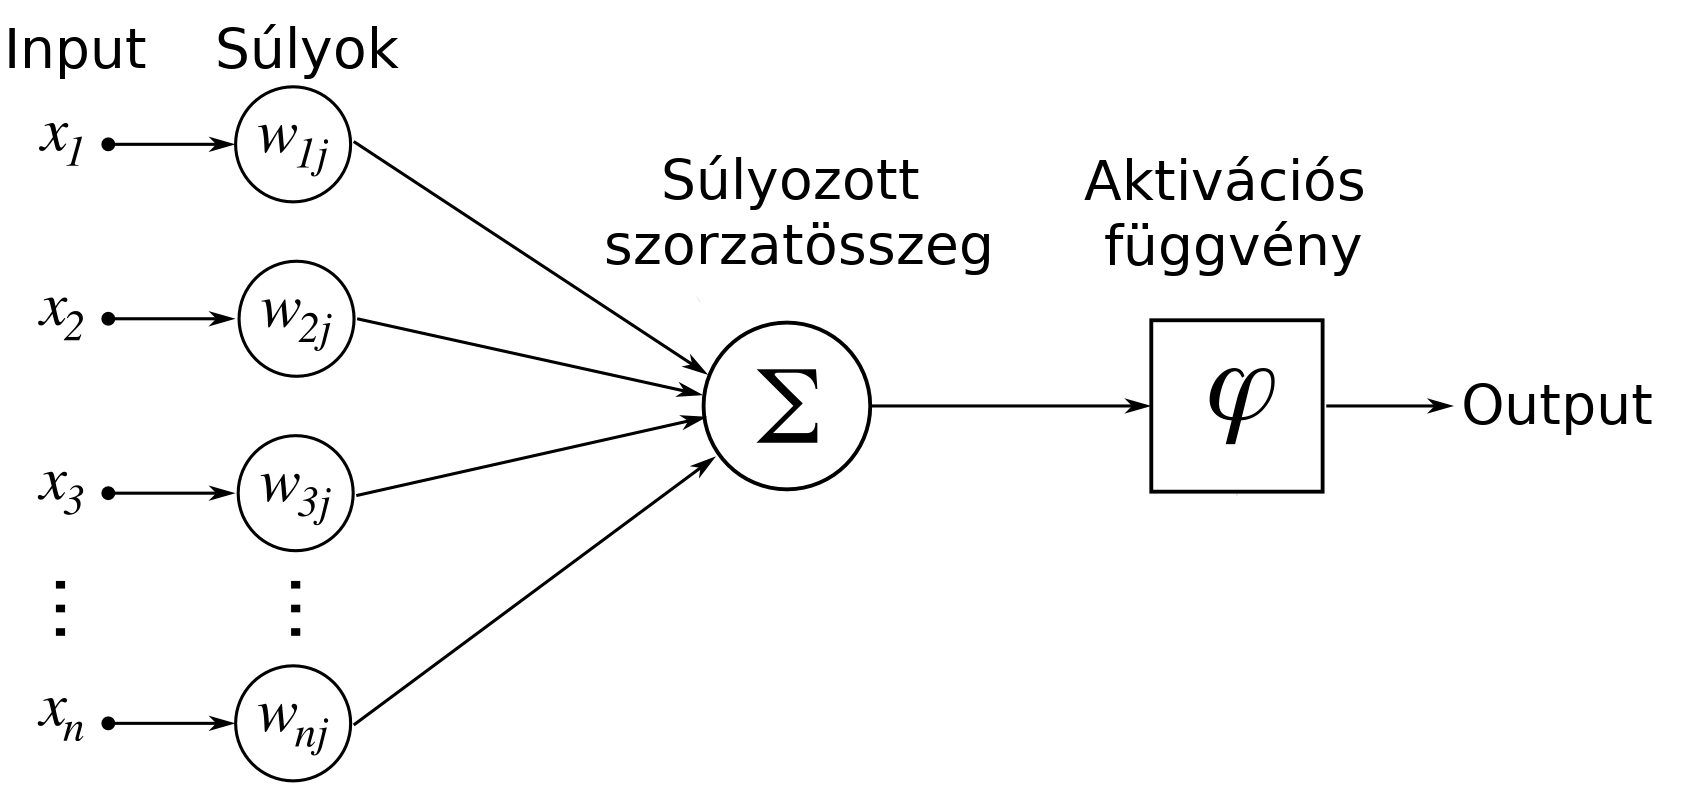
\includegraphics[width=9cm, keepaspectratio]{images/dl_12.png}
\end{center}
\end{column}
\end{columns}
\end{frame}

\begin{frame}{Gyakori aktivációs függvények}
\begin{columns}
\begin{column}{.5\textwidth}
\only<1>{A neuron által kiszámolt súlyozott szorzatösszeg egy aktivációs függvénybe kerül behelyettesítésre. \par\smallskip
A neurális hálózatok az aktivációs függvények segítségével \textbf{sajátítanak el komplex mintázatokat}. Az aktivációs függvény vezeti be a neurális hálózatokba a \textbf{nemlineáris transzformációt}, enélkül csak egy lineáris transzformáció lenne.\par\smallskip
A különböző alkalmazásokra külön aktivációs függvények használatosak.}
\only<2>{
\\
$
Sigmoid(x) = \frac{1}{1 + e^x} 
$\\
\vspace{0.5cm}
$
ReLU(x) = max(0, x)
$\\
\vspace{0.5cm}
$
ELU(x)=\begin{cases}_{\alpha(e^{x}-1)}^{x} & _{ha\:x<0}^{ha\:x\geq0}\end{cases}
$\\
\vspace{0.5cm}
$
tanh(x) = \frac{e^{2x} - 1}{e^{2x} + 1}
$\\
\vspace{0.5cm}
$
Leaky\:ReLU(x)=\begin{cases}
_{\alpha\cdot x}^{x} & _{ha\:x<0}^{ha\:x\geq0}\end{cases}
$\\
\vspace{0.5cm}
$
Swish(x,\beta) = \frac{x}{1 + e^{-\beta \cdot x}}
$\\
}
\end{column}
\begin{column}{.5\textwidth}
\begin{center}
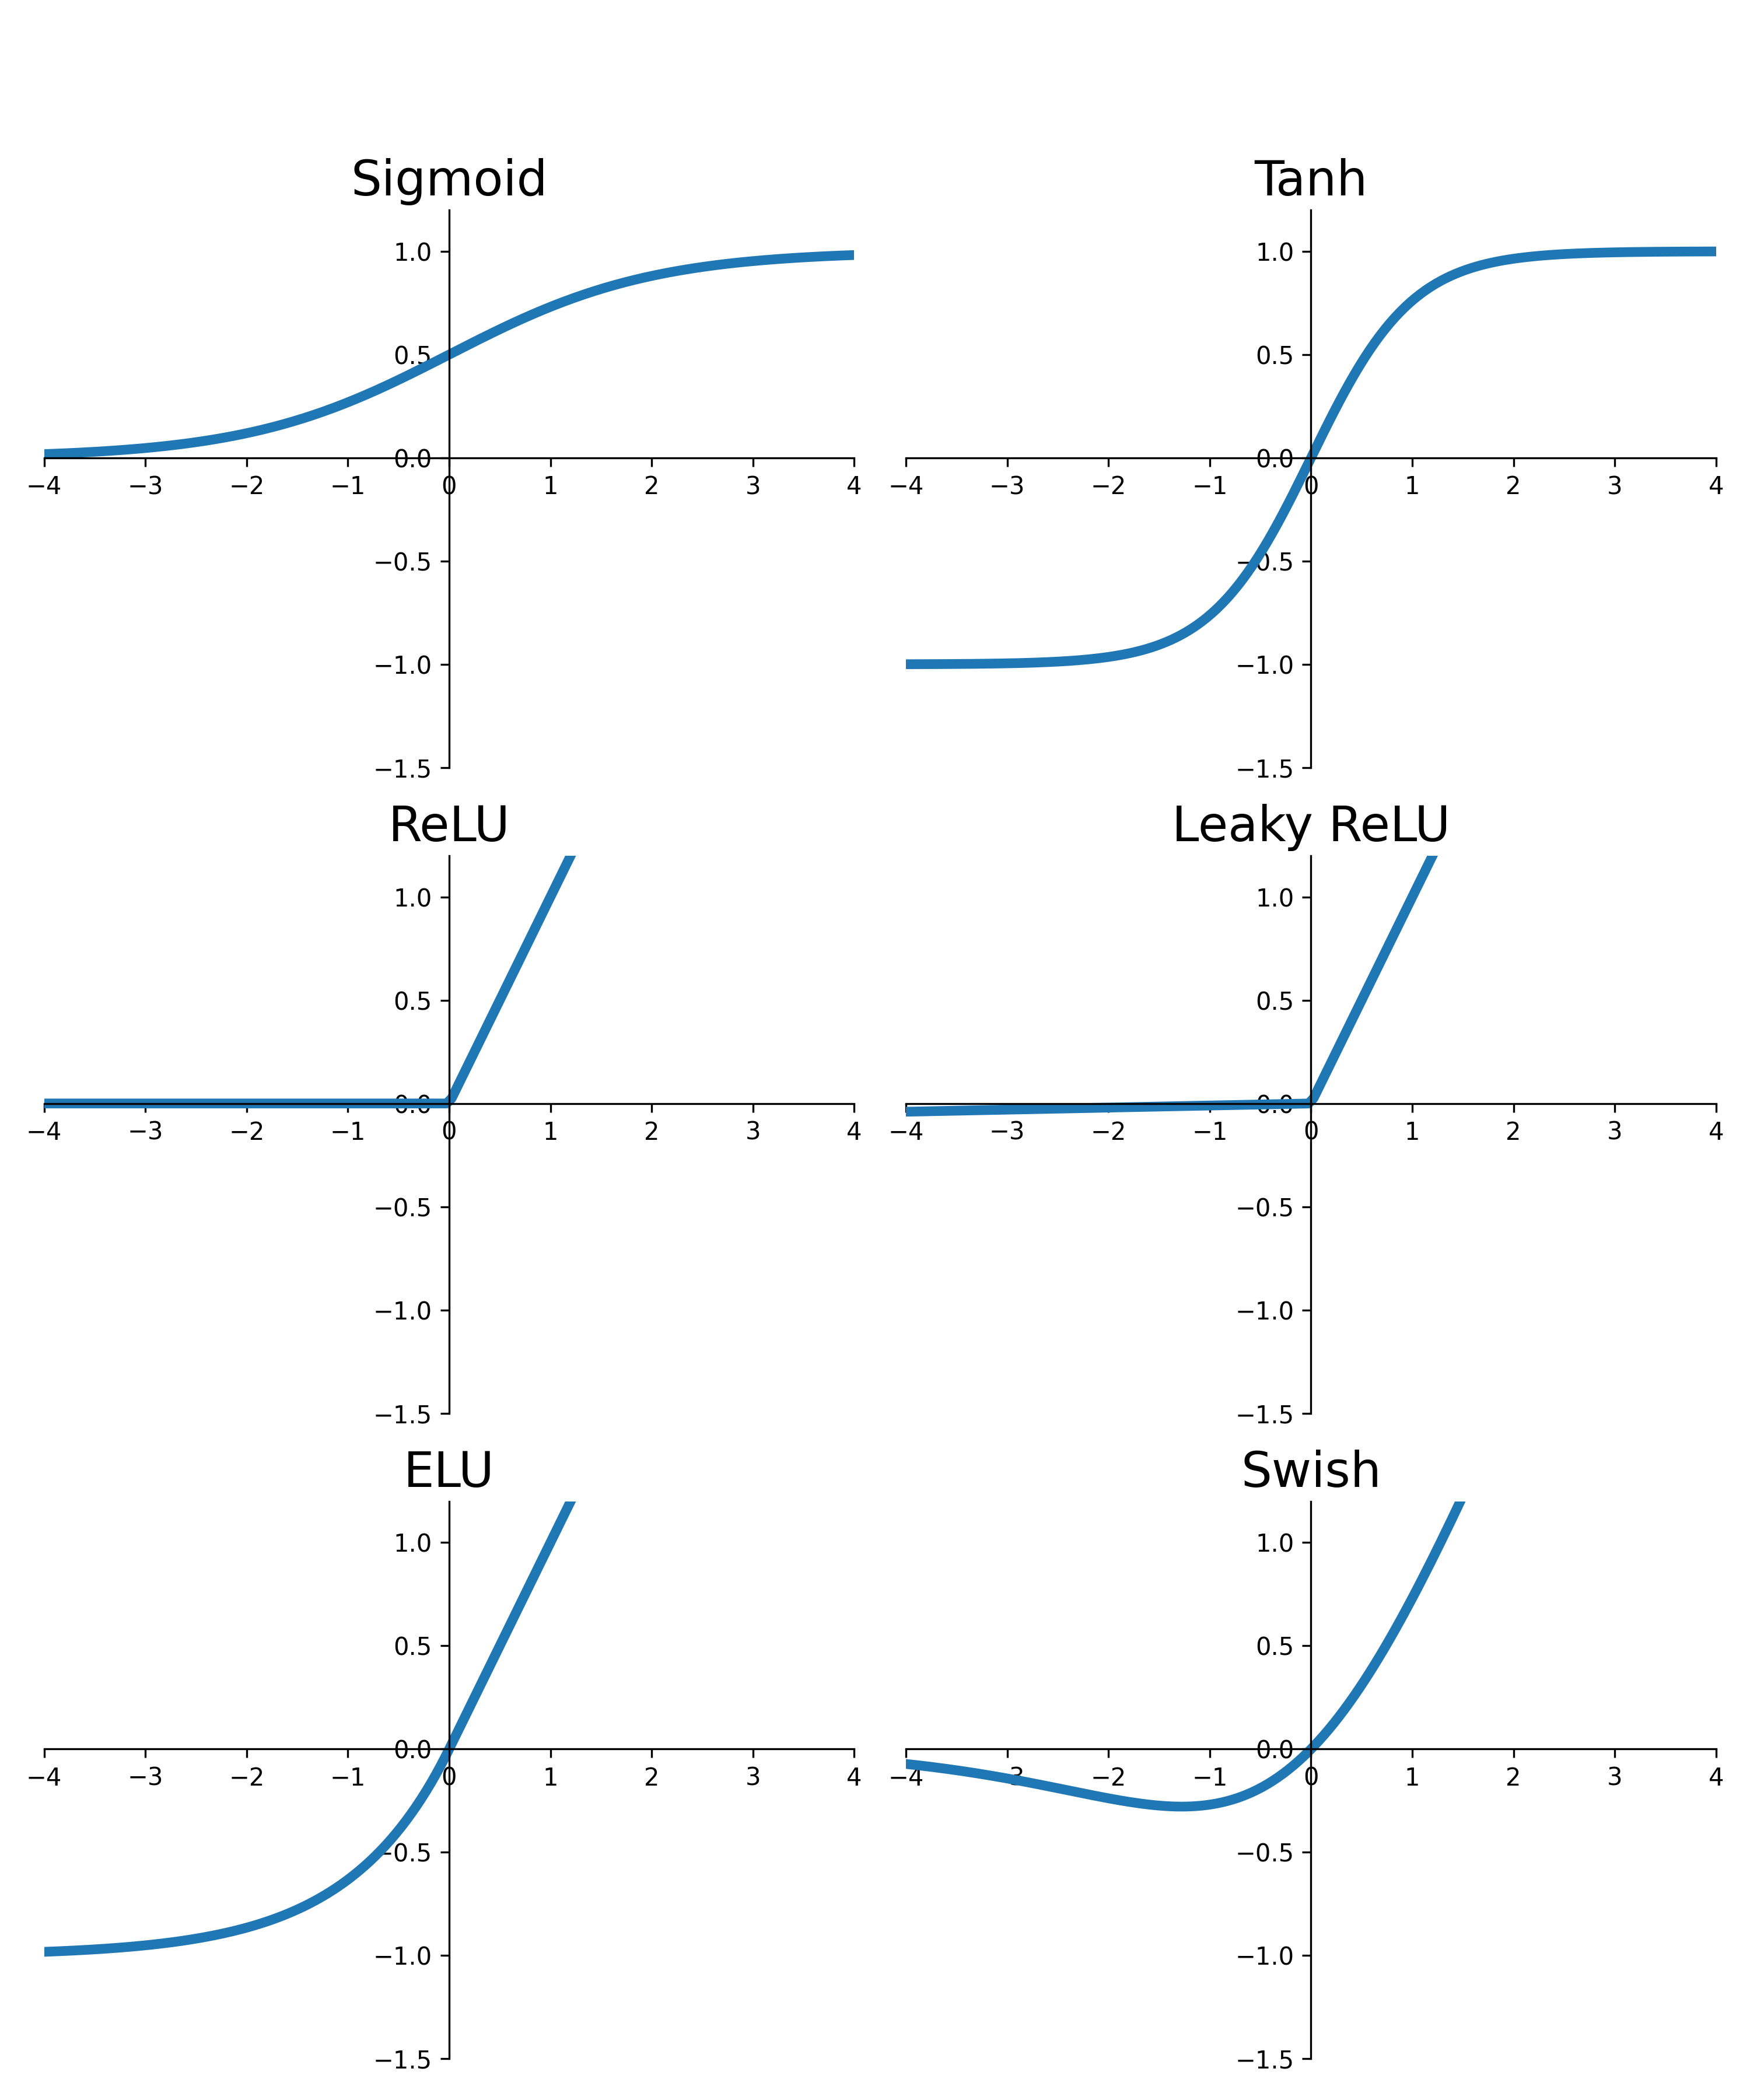
\includegraphics[height=7cm, keepaspectratio]{images/dl_2.png}
\end{center}
\end{column}
\end{columns}
\end{frame}

\begin{frame}{Többrétegű hálózatok}
\begin{columns}
\begin{column}{.5\textwidth}
Ebben az esetben a neuronok rétegekben foglalnak helyet. A kapcsolataik az előző réteg kimeneteivel állnak összeköttetésben. A legelső réteg neuronjai a bemeneti adattal állnak összeköttetésben. Minden bemeneti jellemzőhöz egy neuron tartozik.\par\smallskip
\begin{block}{Teljesen becsatolt neuronréteg kimenete}
\[
h_{W,b}(X)=\varphi(XW+b)
\]
\vspace{-0.5cm}
\begin{itemize}
	\item $X$: Input jellemzők mátrixa
	\item $W$: Kapcsolati súlyok mátrixa
	\item $b$: Torzítások vektora
	\item $\varphi$: Aktivációs függvény
\end{itemize}
\end{block}
\end{column}
\begin{column}{.5\textwidth}
\begin{center}
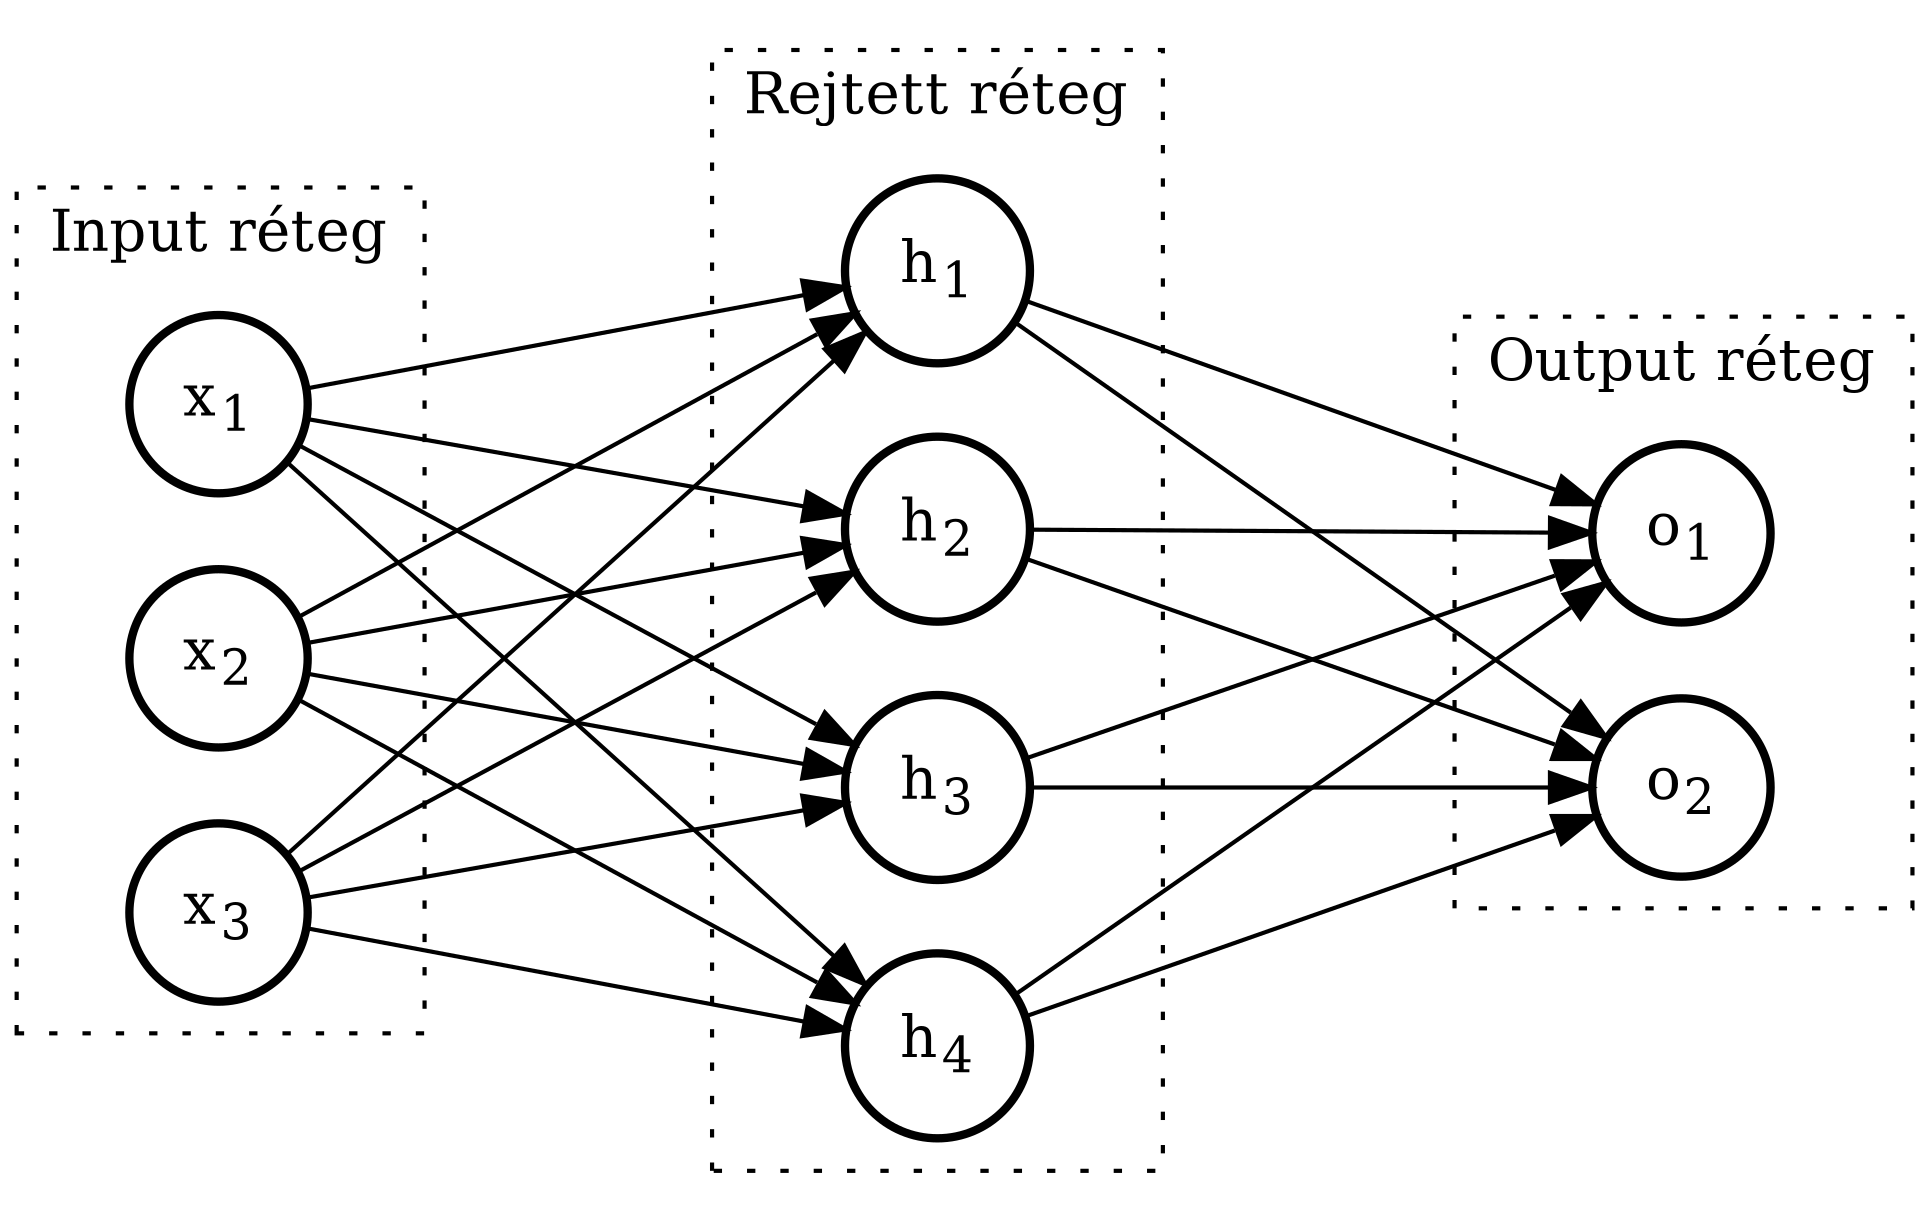
\includegraphics[width=7cm, keepaspectratio]{graphs/dl_0.png}
\end{center}
\end{column}
\end{columns}
\end{frame}

\begin{frame}{Hálózati architektúrák}
\begin{columns}
\begin{column}{.5\textwidth}
\only<1>{A regressziós problémák esetén a neurális hálónak \textbf{egyetlen output neuronja} van.\par\smallskip
A regresszió \textbf{tárgya egy folytonos} változó. Ebben az esetben a neuron output értéke a neurális hálózat predikciója a célváltozóra vonatkozóan.\par\smallskip
\textbf{Például}: hány fok lesz holnap este?\\
- 35.}
\only<2>{Az osztályozási problémák tárgya \textbf{egy diszkrét változó}, amely különálló kategóriákra osztható.\par\smallskip
Az osztályozó hálózatnak \textbf{annyi output neuronja van, ahány kategória lehetséges osztályozás esetén}. A predikció a mintaegyed adott osztályba esésének valószínűségét adja.\par\smallskip
\textbf{Például}: meleg vagy hideg lesz az idő holnap este?\\
- Hideg.}
\end{column}
\begin{column}{.5\textwidth}
\only<1>{\begin{center}
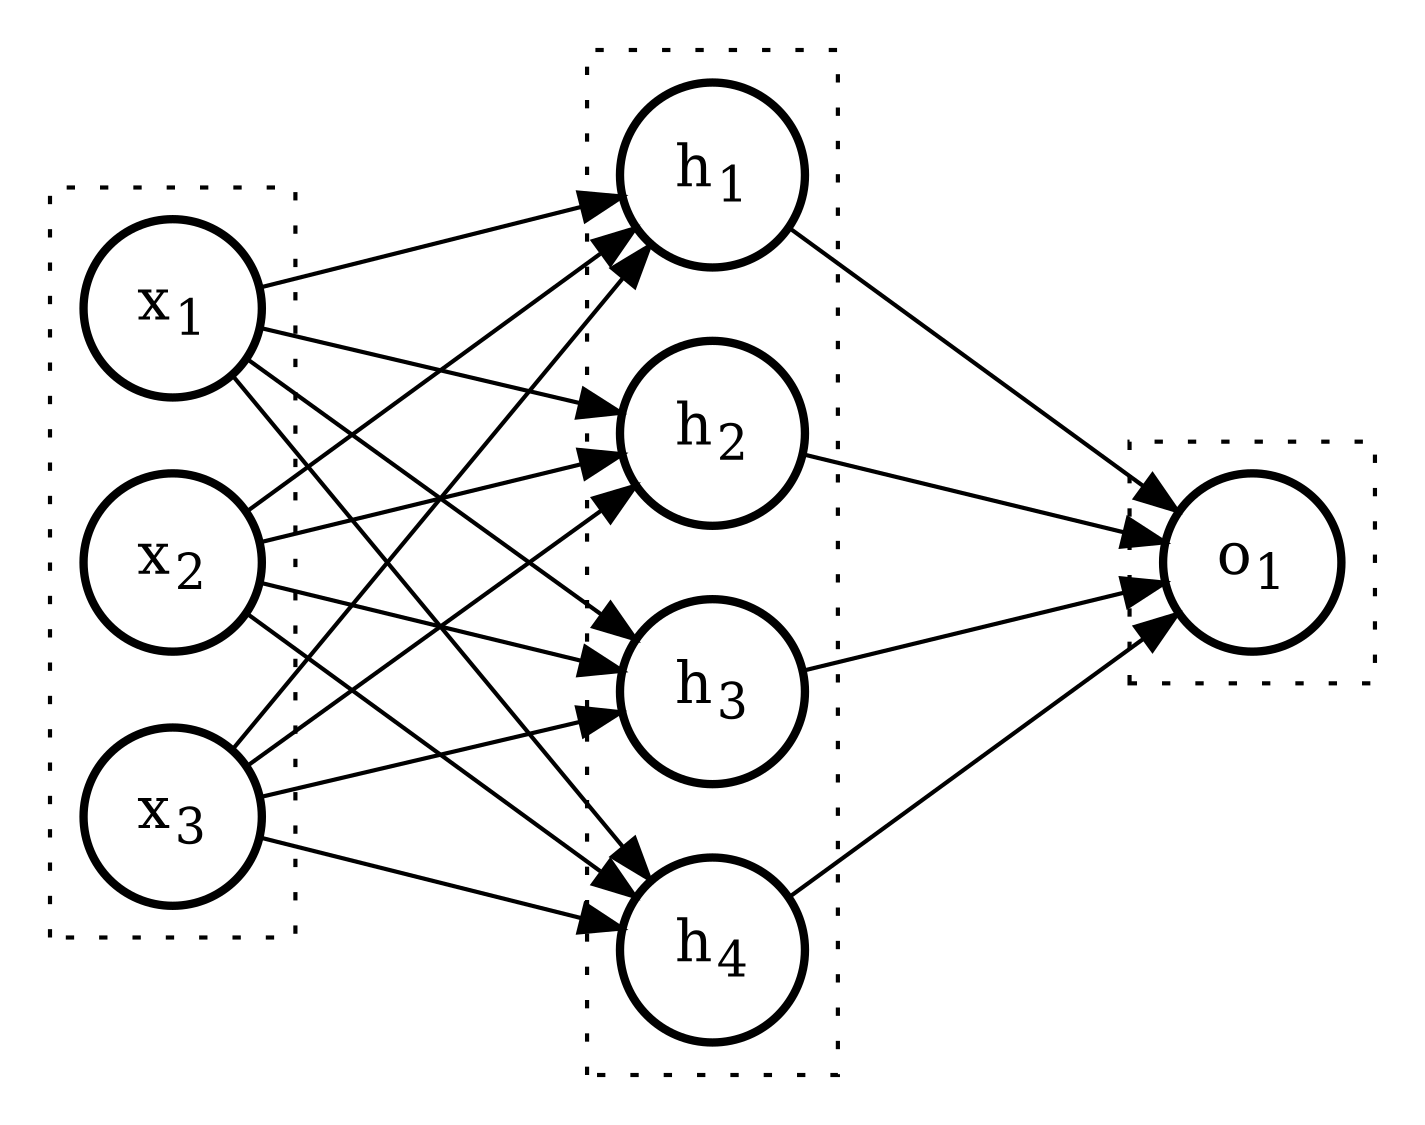
\includegraphics[width=7cm, keepaspectratio]{graphs/dl_2.png}
\end{center}}
\only<2>{\begin{center}
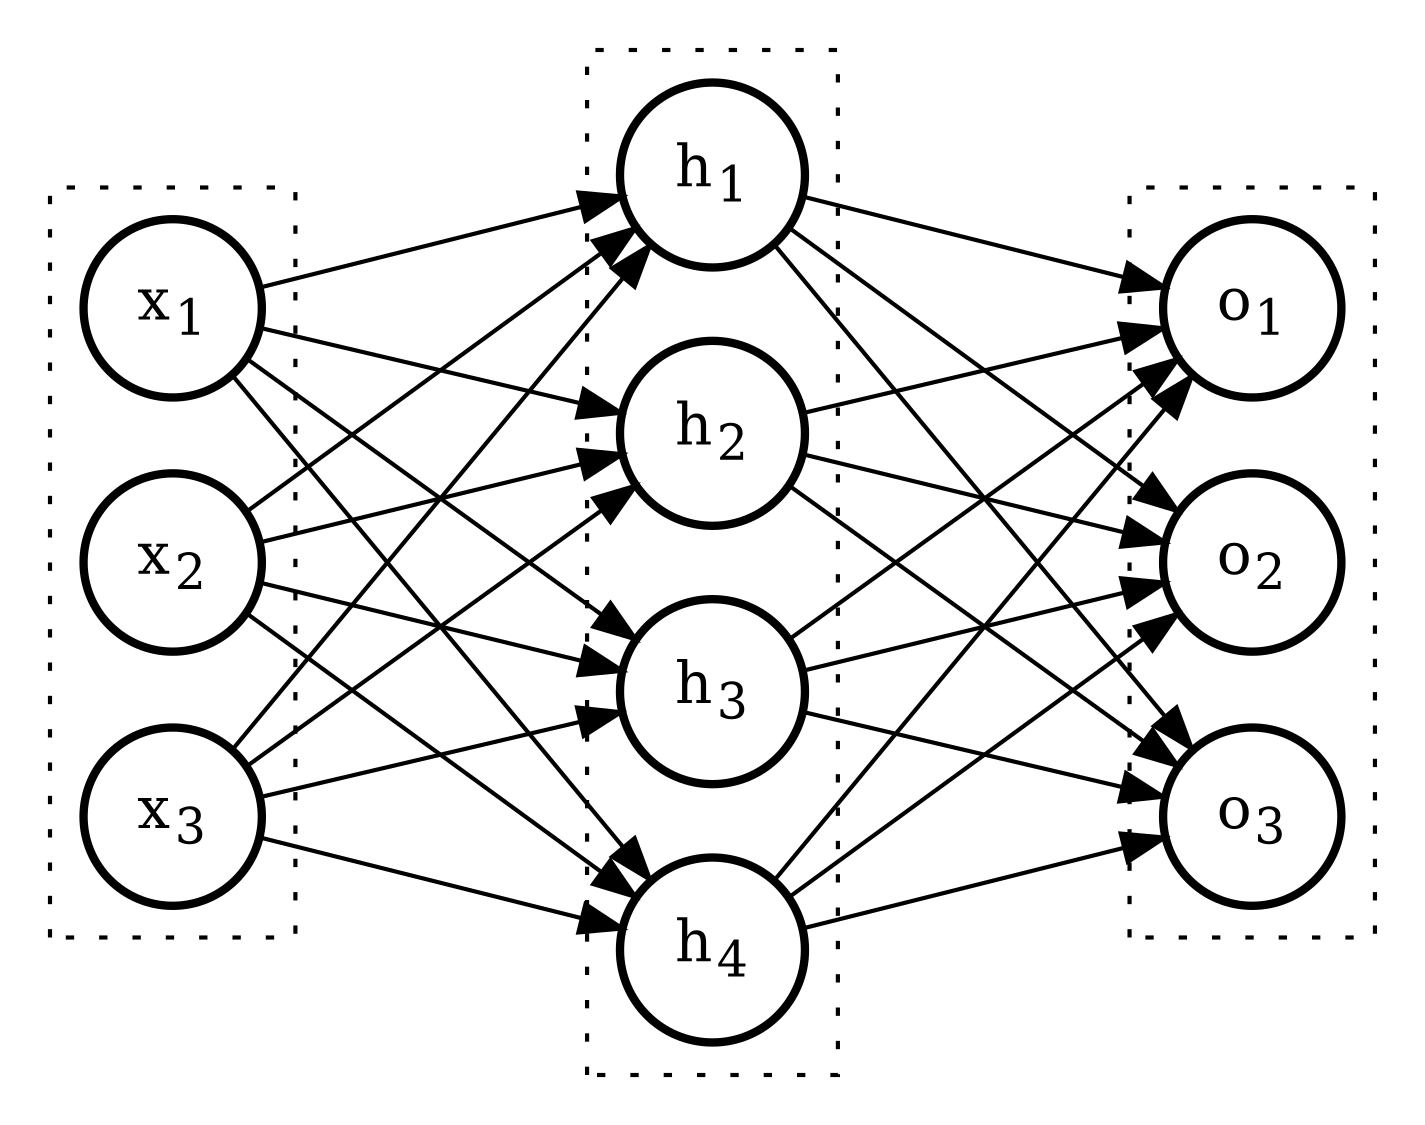
\includegraphics[width=7cm, keepaspectratio]{graphs/dl_1.png}
\end{center}}
\end{column}
\end{columns}
\end{frame}

\section{Tanítás}

\begin{frame}
\tableofcontents[currentsection]
\end{frame}

\begin{frame}{Transzfertanulás}
\begin{columns}
\begin{column}{.5\textwidth}
Neurális hálózatok esetén lehetséges más neurális hálózatok \textbf{előretanított súlyainak felhasználása}. Ebben az esetben adott rétegek kimaradnak a tanításból.\par\smallskip
Jellemzően az alsó rétegek lesznek rögzítettek, és a felső rétegek pedig tanítottak. Ez lehetőséget ad a hálózatnak \textbf{új mintázatokat megismerni hasonló feladatok} esetén.
\end{column}
\begin{column}{.5\textwidth}
\begin{center}
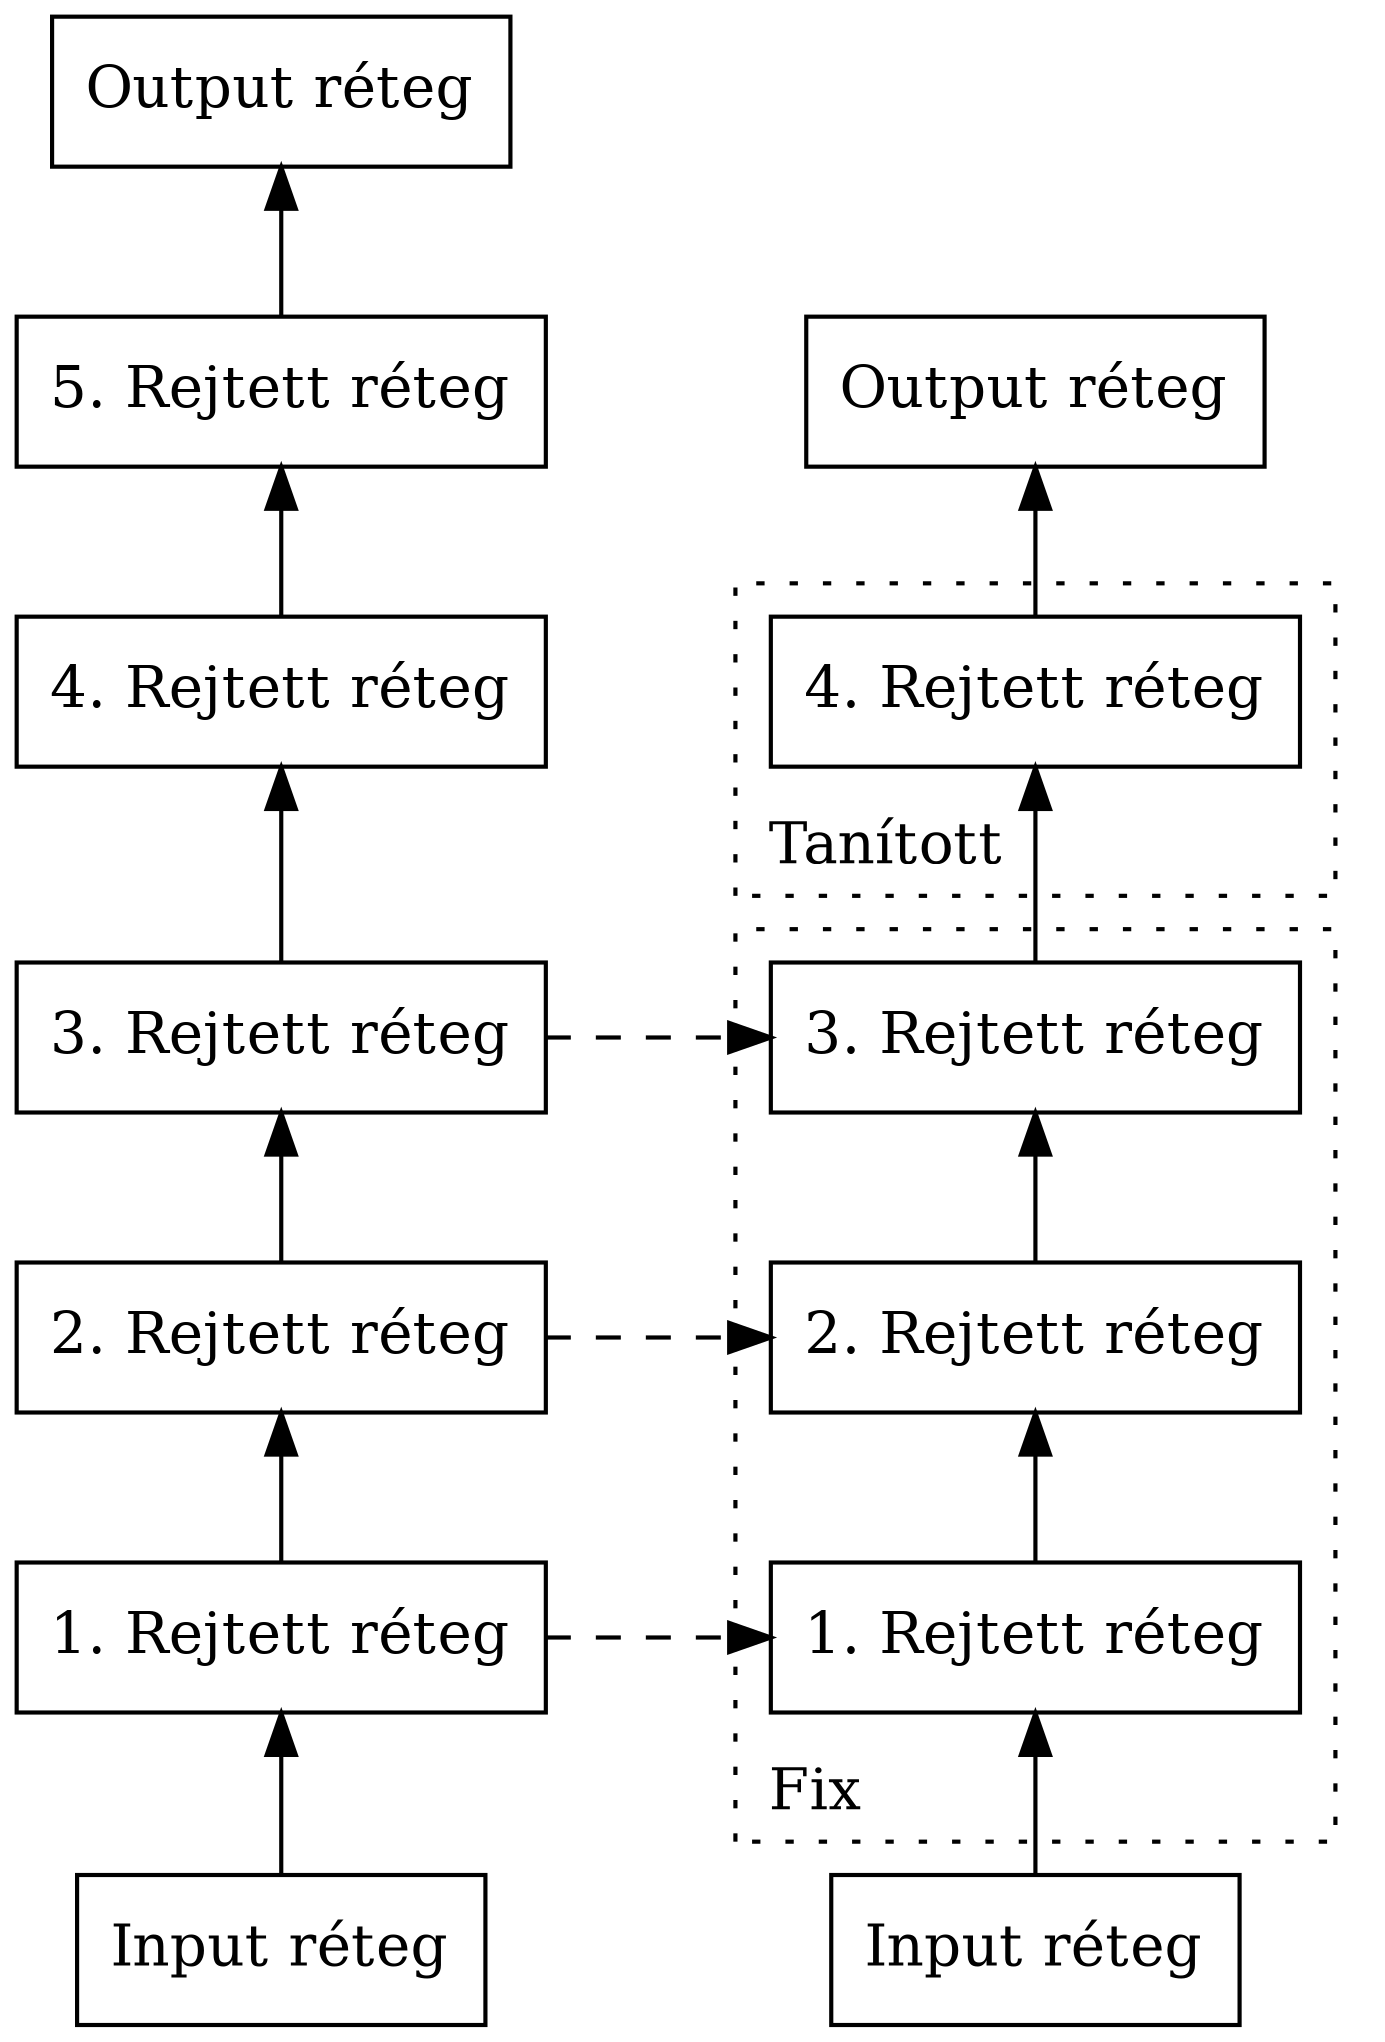
\includegraphics[height=7cm, keepaspectratio]{graphs/dl_3.png}
\end{center}
\end{column}
\end{columns}
\end{frame}

\begin{frame}{Optimalizációs algoritmusok}
\begin{columns}
\begin{column}{.5\textwidth}
A matematikában az optimalizációs algoritmusok célja megtalálni a legjobb megoldást egy olyan problémára, ahol valamilyen korlátozásokkal kell \textbf{egy célfüggvényt minimalizálni}.\par\smallskip
Mivel a neurális hálók által reprezentált nemlineáris függvények minimum helyei nem számíthatók ki zárt formájú függvénnyel mint pl. a másodfokú függvény esetén, iteratív optimalizációs algoritmusokra van szükség. 
\end{column}
\begin{column}{.5\textwidth}
\begin{center}
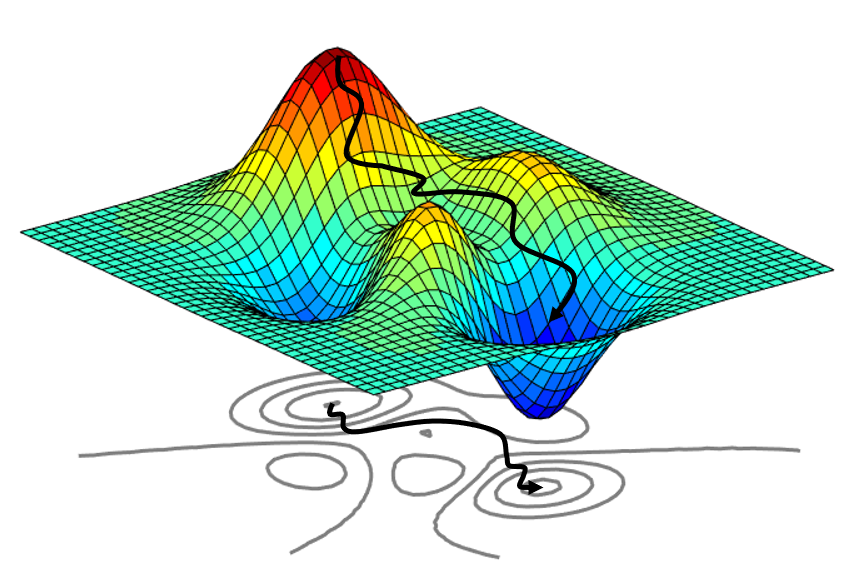
\includegraphics[height=7cm, width=7cm, keepaspectratio]{images/dl_8.png}
\end{center}
\end{column}
\end{columns}
\end{frame}

\begin{frame}{Kötegelt gradiens ereszkedés}
\begin{columns}
\begin{column}{.7\textwidth}
\begin{algorithm}[H]
\caption{Kötegelt gradiens ereszkedés}
\SetAlgoLined
\textbf{Input}: $\alpha$ tanulási sebesség, $f(\theta)$ célfüggvény\\
$\theta_0 \leftarrow 0$\tcc*[t]{Paraméterek inicializálása} 
\For{$t = 0 \rightarrow max_t$}{
	$\nabla f(\theta_t)$ gradiens kiszámítása\;
	$\theta_{t+1} = \theta_t - \alpha \cdot \nabla f(\theta_t)$\;
}
\end{algorithm}
Ahol $\theta$ a célfüggvényt meghatározó paraméterek vektora, $\nabla f(\theta_t)$ a célfüggvény gradiense, $\alpha \in [0,1]$ a tanulási sebesség.
\end{column}
\begin{column}{.3\textwidth}
\begin{center}
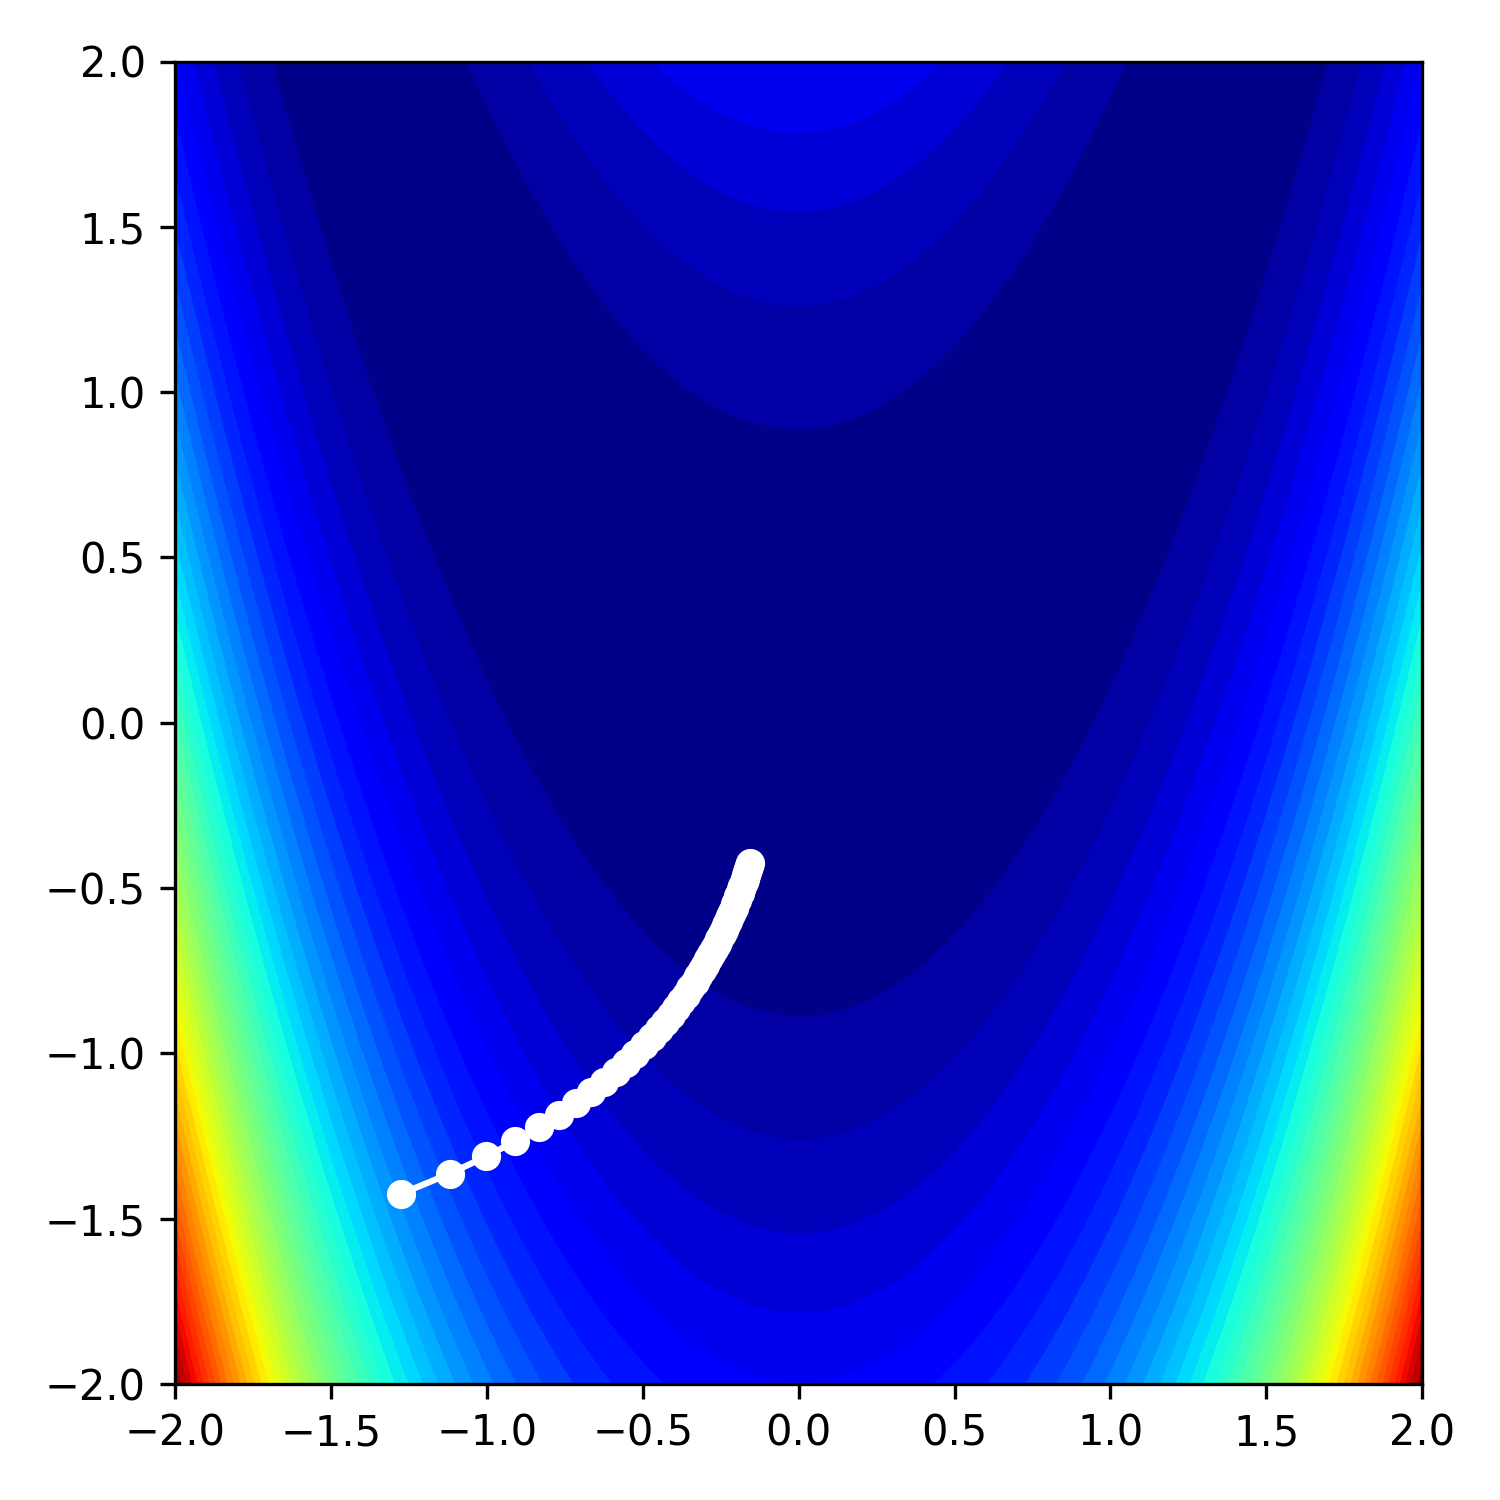
\includegraphics[height=5cm, width=5cm, keepaspectratio]{images/gd_batch.png}
\end{center}
\end{column}
\end{columns}
\end{frame}

\begin{frame}{Mini-kötegelt gradiens ereszkedés}
\begin{columns}
\begin{column}{.7\textwidth}
\begin{algorithm}[H]
\caption{Mini-kötegelt gradiens ereszkedés}
\SetAlgoLined
\textbf{Input}: $\alpha$ tanulási sebesség, $f(\theta)$ célfüggvény\\
$\theta_0 \leftarrow 0$\tcc*[t]{Paraméterek inicializálása} 
\For{$t = 0 \rightarrow max_t$}{
	$B$ miniköteg mintázása a tanító halmazból\;
	$\nabla f(\theta_t,B)$ gradiens kiszámítása a minikötegen\;
	$\theta_{t+1} = \theta_t - \alpha \cdot \nabla f(\theta_t,B)$\;
}
\end{algorithm}
Ahol $B$ a teljes tanító halmazból vett véletlenszerű minta. A minta számosságát hiperparaméter szabályozza. 
\end{column}
\begin{column}{.3\textwidth}
\begin{center}
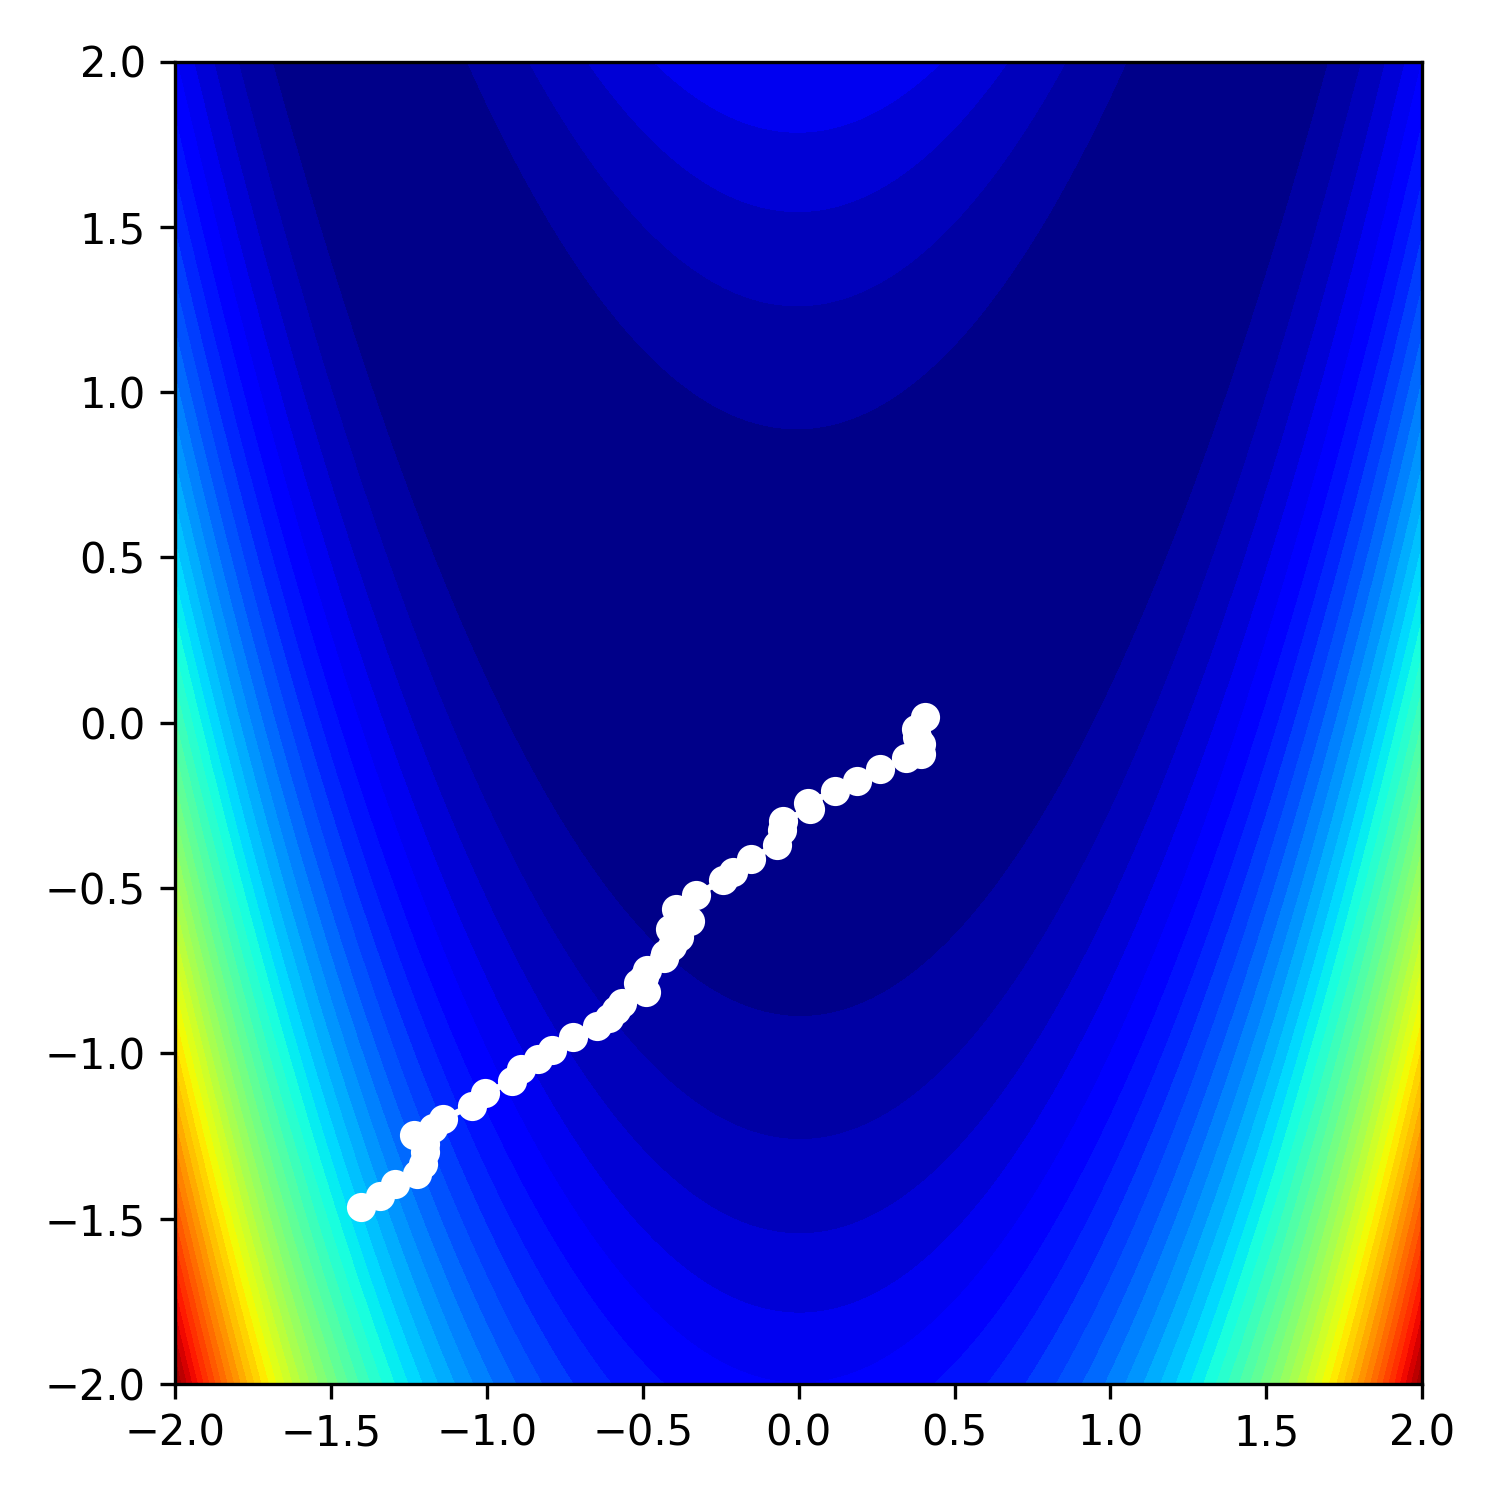
\includegraphics[height=5cm, width=5cm, keepaspectratio]{images/gd_minibatch.png}
\end{center}
\end{column}
\end{columns}
\end{frame}

\begin{frame}{Sztochasztikus gradiens ereszkedés}
\begin{columns}
\begin{column}{.7\textwidth}
\begin{algorithm}[H]
\caption{Sztochasztikus gradiens ereszkedés}
\SetAlgoLined
\textbf{Input}: $\alpha$ tanulási sebesség, $f(\theta)$ célfüggvény\\
$\theta_0 \leftarrow 0$\tcc*[t]{Paraméterek inicializálása} 
\For{$t = 0 \rightarrow max_t$}{
	$p$ adatpont kiválasztása az adathalmazból\;
	$\nabla f(\theta_t,p)$ gradiens kiszámítása a pontban\;
	$\theta_{t+1} = \theta_t - \alpha \cdot \nabla f(\theta_t,p)$\;
}
\end{algorithm}
\end{column}
\begin{column}{.3\textwidth}
\begin{center}
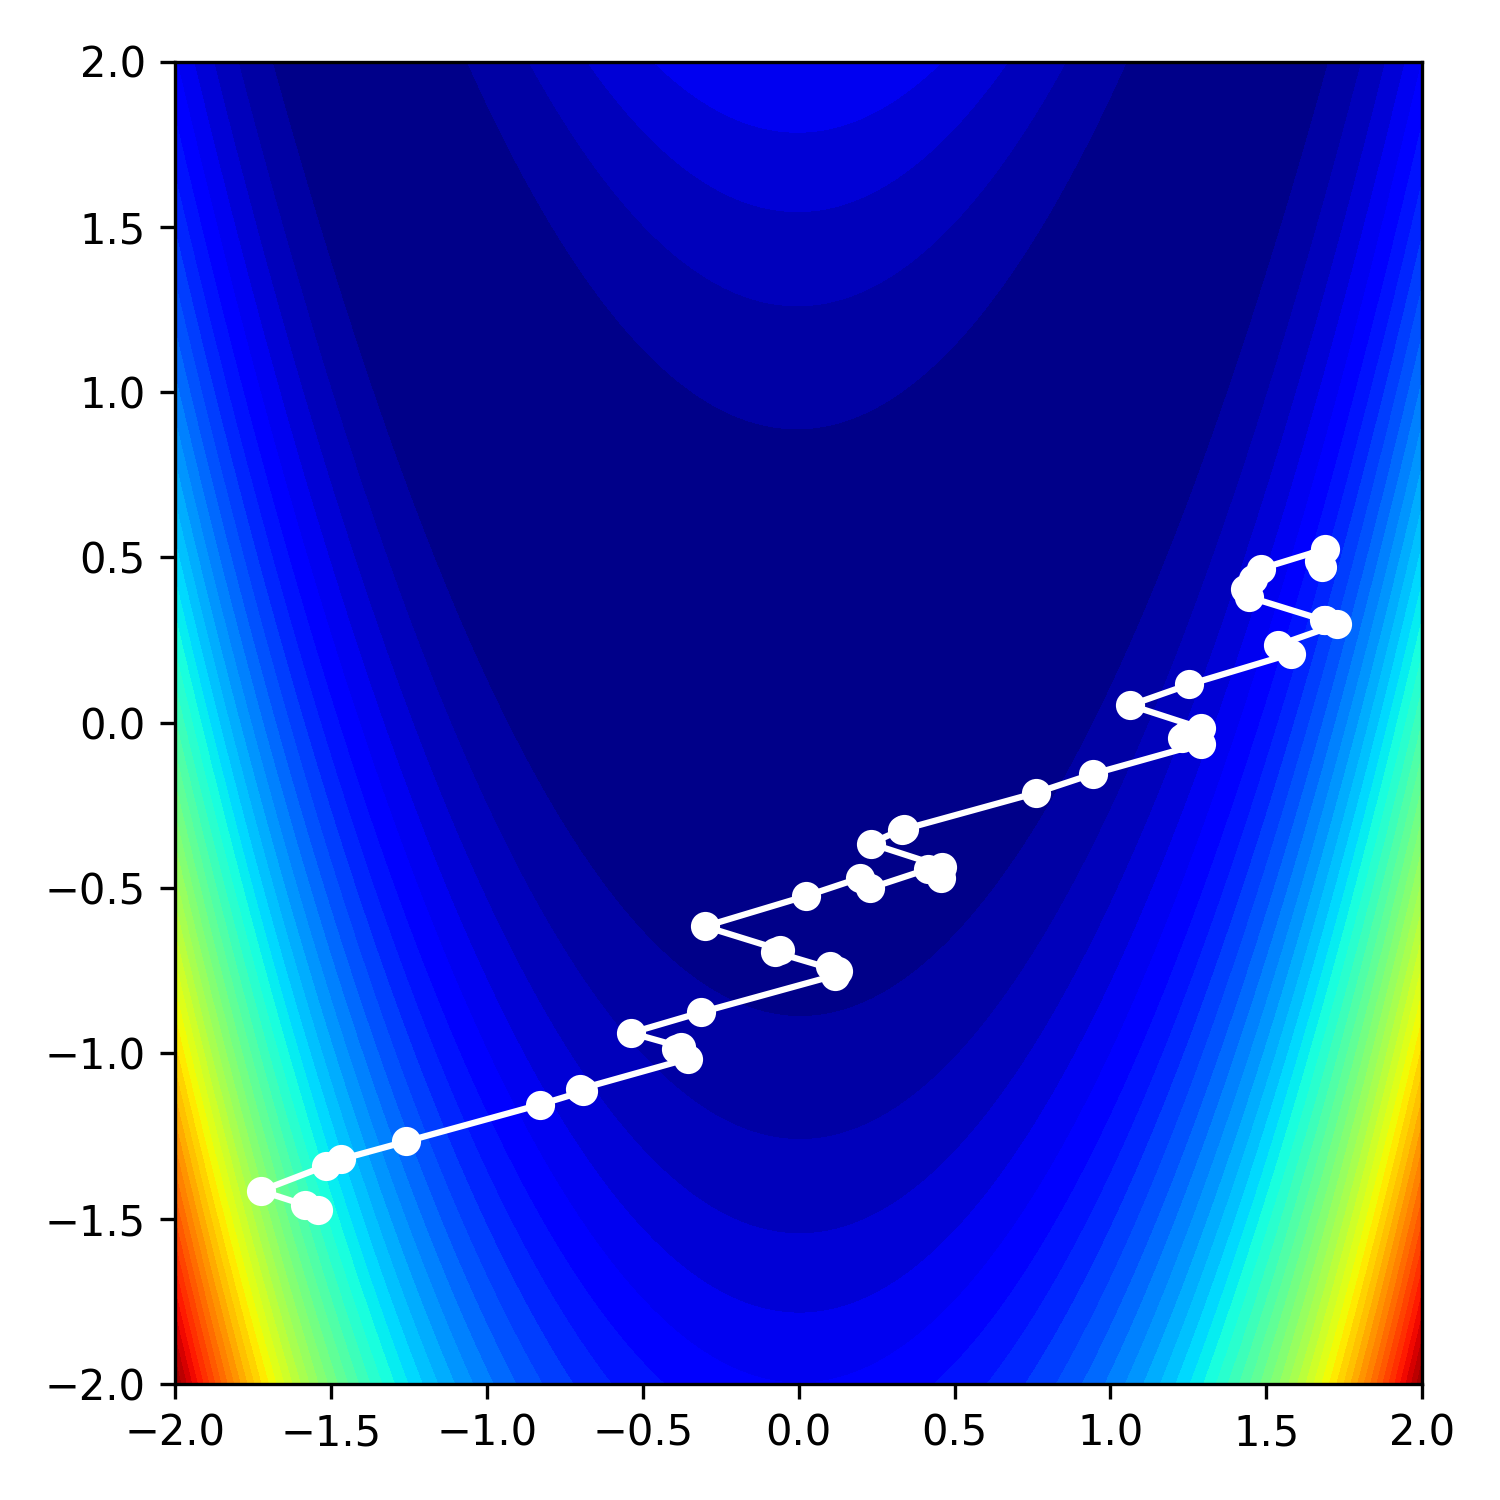
\includegraphics[height=5cm, width=5cm, keepaspectratio]{images/gd_stochastic.png}
\end{center}
\end{column}
\end{columns}
\end{frame}

\begin{frame}{Momentum gradiens ereszkedés}
\begin{columns}
\begin{column}{.7\textwidth}
\begin{algorithm}[H]
\SetAlgoLined
\caption{Momentum gradiens ereszkedés}
\textbf{Input}: $\alpha$ tanulási sebesség, $\beta$ lendület komponens\\
$f(\theta)$ célfüggvény\\
$\theta_0 \leftarrow 0$\tcc*[t]{Paraméterek inicializálása}
$v \leftarrow 0$\tcc*[t]{Sebesség komponens inicializálása}
\For{$t = 0 \rightarrow max_t$}{
	$\nabla f(\theta_t)$ gradiens kiszámítása\;
	$v \leftarrow v \cdot \beta + (1-v) \cdot \nabla f(\theta)$\;
	$\theta_{t+1} \leftarrow \theta_t - \alpha \cdot v$\tcc*[t]{Paraméterek frissítése}
}
\end{algorithm}
A $v$ sebesség komponens akkumulálja a súlyozott múltbeli gradienseket, ezért fog hasonlítani az optimalizáció röppályája egy való életben elgurított golyóéra, amire érvényesek a newtoni mechanika elvei. 
\end{column}
\begin{column}{.3\textwidth}
\begin{center}
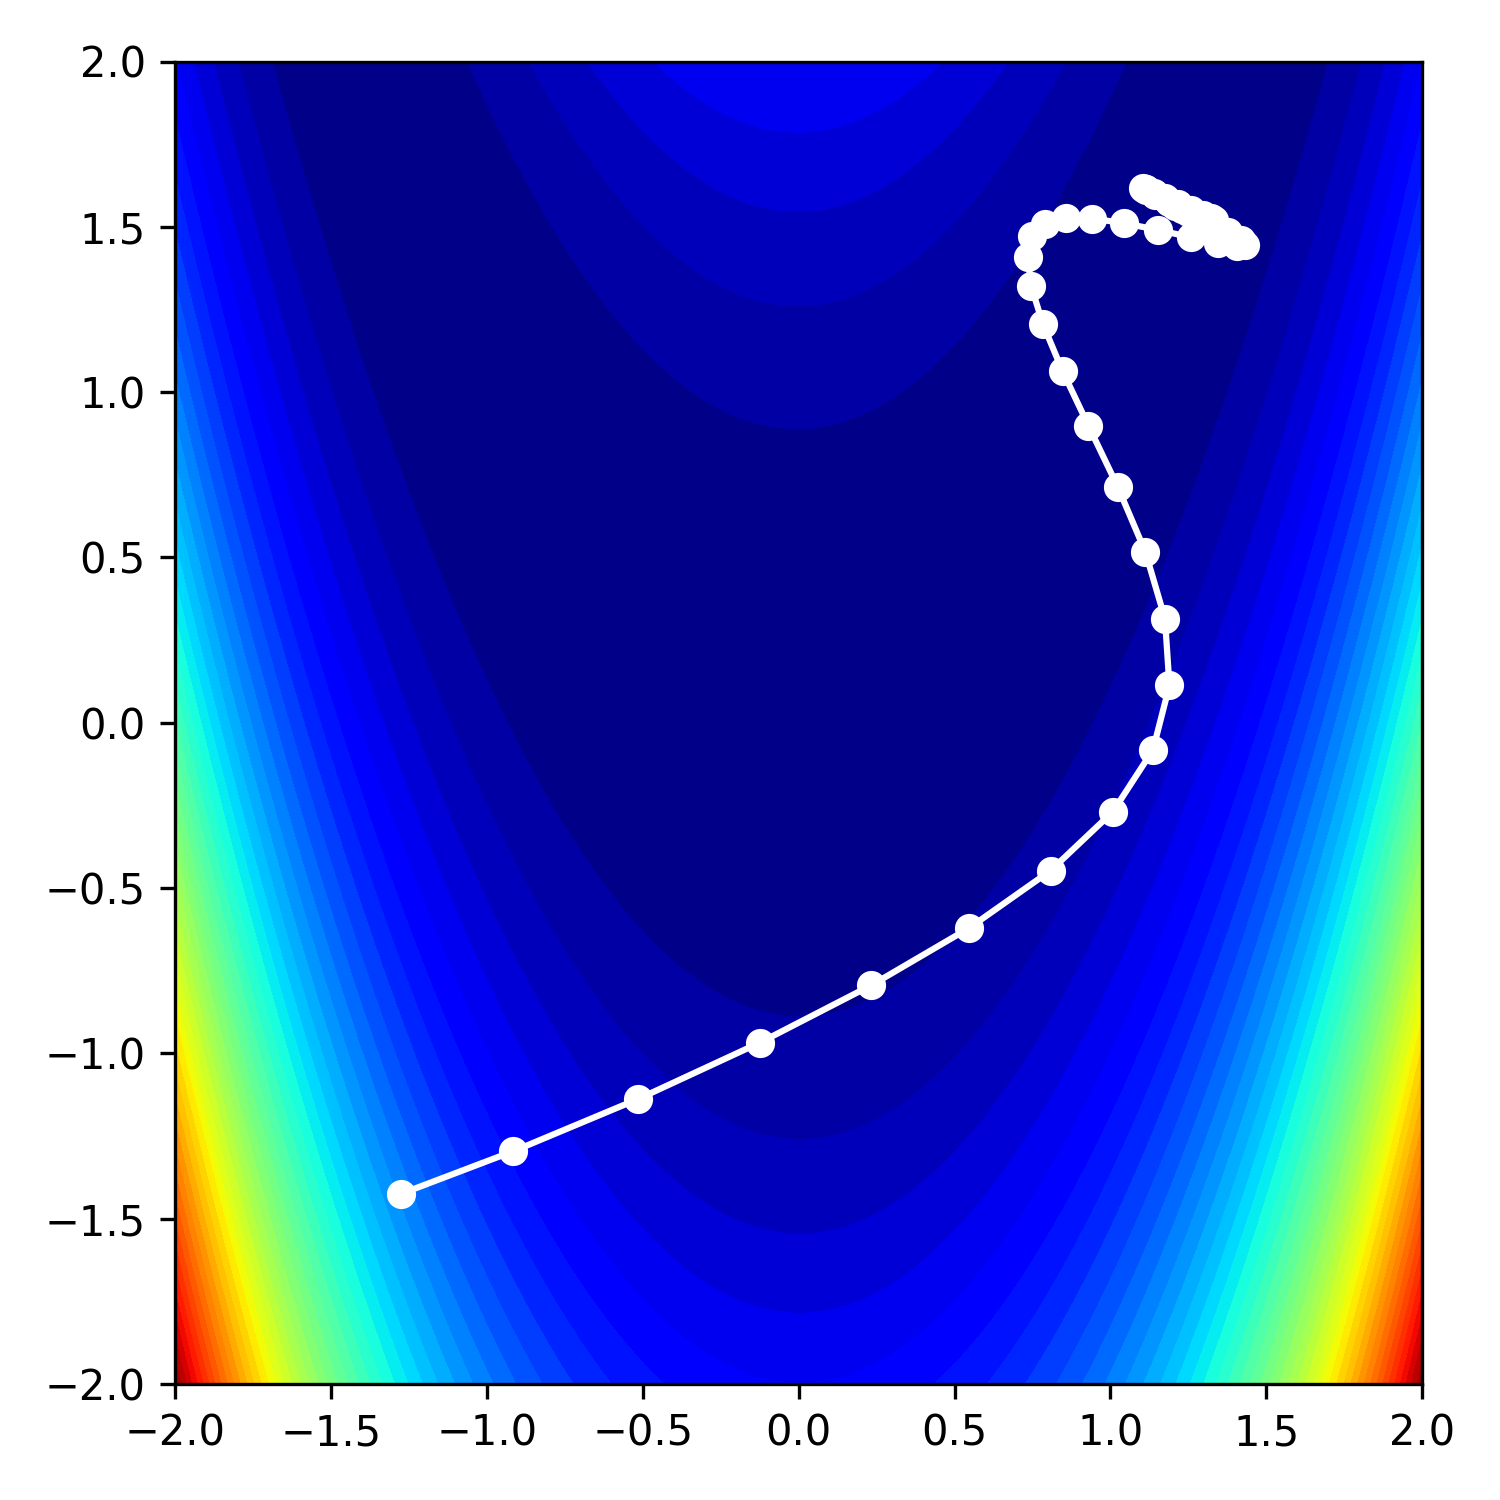
\includegraphics[width=5cm, height=5cm, keepaspectratio]{images/gd_momentum.png}
\end{center}
\end{column}
\end{columns}
\end{frame}

\begin{frame}{Hiba-visszaáramoltató algoritmus neurális hálózat súlyok tanítására}
\begin{enumerate}
	\item \textbf{Inicializáció}: súlyok és torzítások kezdőértékeinek véletlenszerű megadása
	\item \textbf{Előreáramoltatás}: rétegek output értékének kiszámítása: 
	\begin{itemize}
		\item Rejtett réteg: $h_h = \varphi(W_h \cdot x + b_h)$
		\item Output réteg: $h_o = \varphi(W_o \cdot h_h + b_o)$
	\end{itemize}
	\item \textbf{Költség kiszámítása}: regresszió esetén pl.: $MSE = \sum \left( h_o - y \right)^2$
	\item \textbf{Visszaáramoltatás}: 
	\begin{itemize}
		\item Rejtett réteg hibája: $\delta_h=(W_o \cdot \delta_o) \odot \varphi(z_h)$
		\item Output réteg hibája: $\delta_o=(h_o - y) \odot \varphi(z_o)$
	\end{itemize}
	\item \textbf{Gradiens ereszkedés} a súlyokon és torzításokon:
	\begin{itemize}
		\item Rejtett réteg: $W_h \leftarrow W_h - \alpha \cdot \delta_h \cdot x^\top$
		\item Rejtett réteg: $b_h \leftarrow b_h - \alpha \cdot \delta_h$	
		\item Output réteg: $W_o \leftarrow W_o - \alpha \cdot \delta_o \cdot h_o^\top$
		\item Output réteg: $b_o \leftarrow b_o - \alpha \cdot \delta_o$

	\end{itemize}
	\item \textbf{Ismétlés} a meghatározott lépésszámig
\end{enumerate}
\end{frame}

\section{Konvolúciós hálózatok}

\begin{frame}
\tableofcontents[currentsection]
\end{frame}

\begin{frame}{A konvolúció művelete}
\begin{columns}
\begin{column}{.6\textwidth}
A konvolúció egy matematikai művelet, ami két függvényt kombinál egy harmadikká. Egy \textbf{jelfüggvényt} valamilyen \textbf{magfüggvénnyel} vegyít egy outputtá, ami megadja, hogy \textbf{a mag mennyiben befolyásolja a jelet}. 
\begin{block}{Konvolúció (2D, diszkrét)}
A diszkrét konvolúció két 2D tömbön értelmezett, és jellemzők kivonatolására, szűrők alkalmazására használatos. Konvolúció $f$ jelen és $g$ magon, $i,j$ képkoordinátákra:
\[
(f \textasteriskcentered g)[i, j] = \sum_{m=-\infty}^\infty \sum_{n=-\infty}^\infty g[i-m, j-n]f[m,n]
\]
\end{block}
\end{column}
\begin{column}{.4\textwidth}
\begin{center}
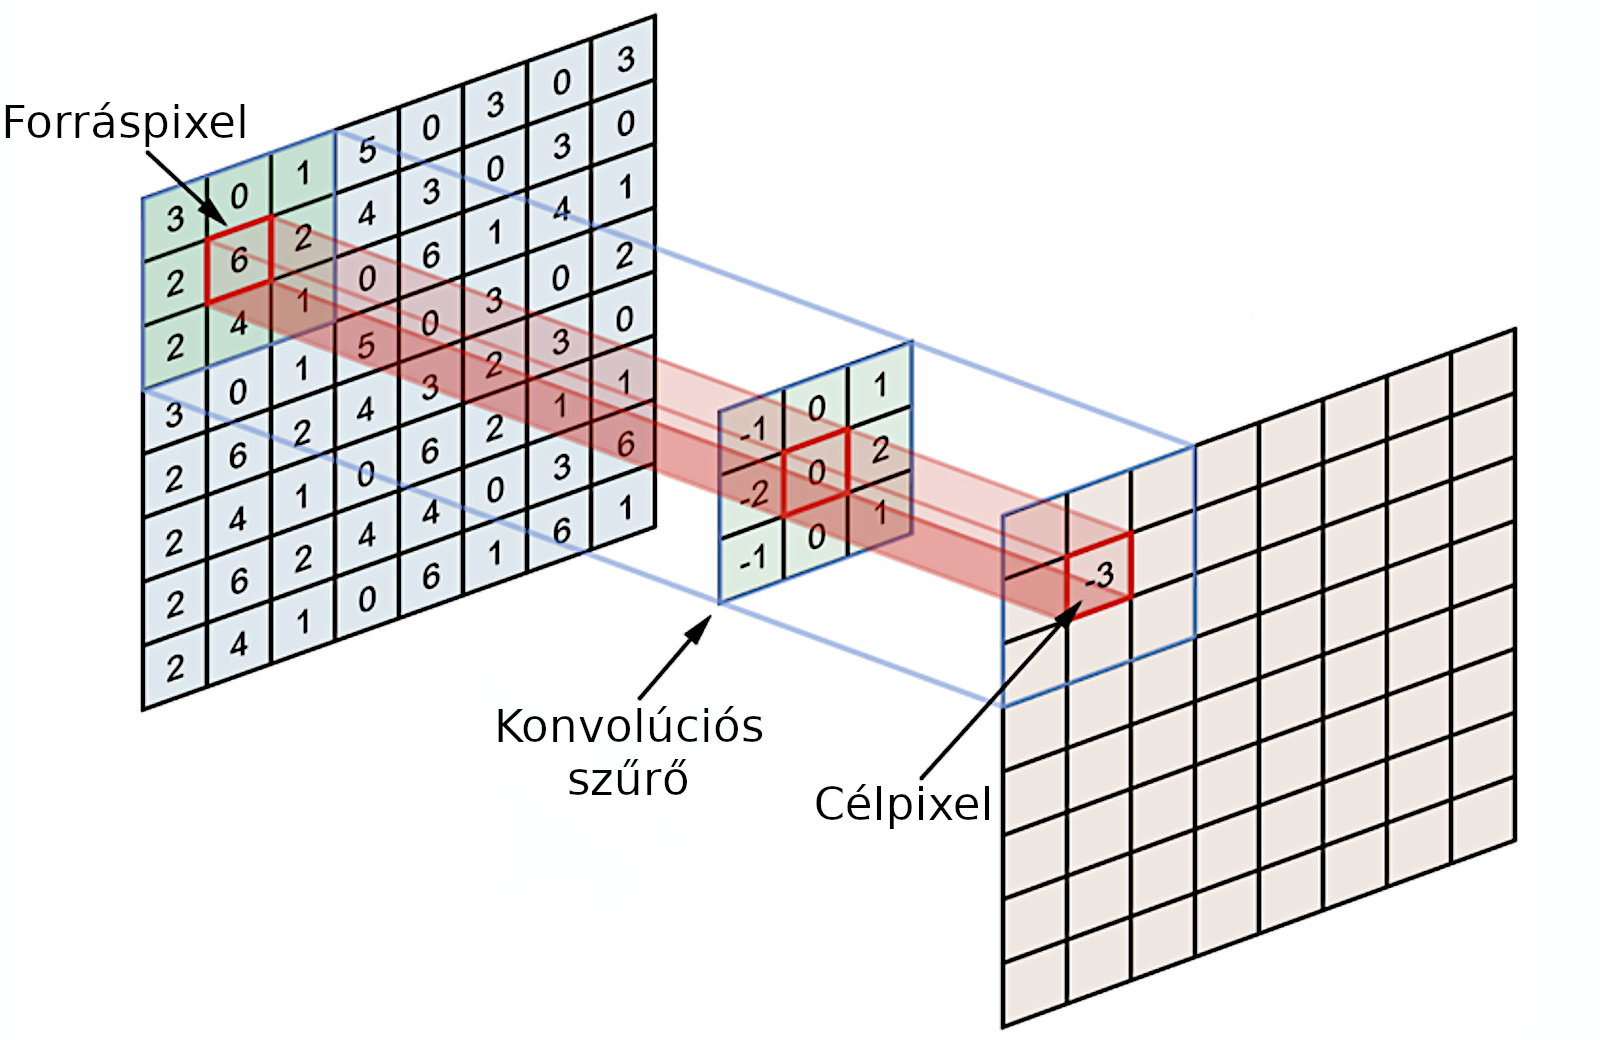
\includegraphics[height=6cm, width=6cm, keepaspectratio]{images/dl_3.png}
\end{center}
$(-1 \cdot 3) + (0 \cdot 0) + (1 \cdot 1) +$\\
$(-2 \cdot 2) + (0 \cdot 6) + (2 \cdot 2) +$\\
$(-1 \cdot 2) + (0 \cdot 4) + (1 \cdot 1) = -3$\\
\end{column}
\end{columns}
\end{frame}

\begin{frame}{A konvolúciós réteg}
\begin{columns}
\begin{column}{.5\textwidth}
A neurális hálózatok konvolúciós rétegeiben a \textbf{tanítható súlyok az egyes forráspixelekhez tartozó konvolúciós szűrőkben elhelyezkedő értékek}. Ez minden forráspixelhez egy egyedi szűrőt jelent, de lehetséges tetszőleges számú szűrő is.\par\smallskip
A konvolúciós magfüggvények szűrőként is alkalmazhatók. Például a képen egy élkereső szűrő látható, ami az outputra az input képen található élek másolódnak át.\par\smallskip  
\end{column}
\begin{column}{.5\textwidth}
\begin{center}
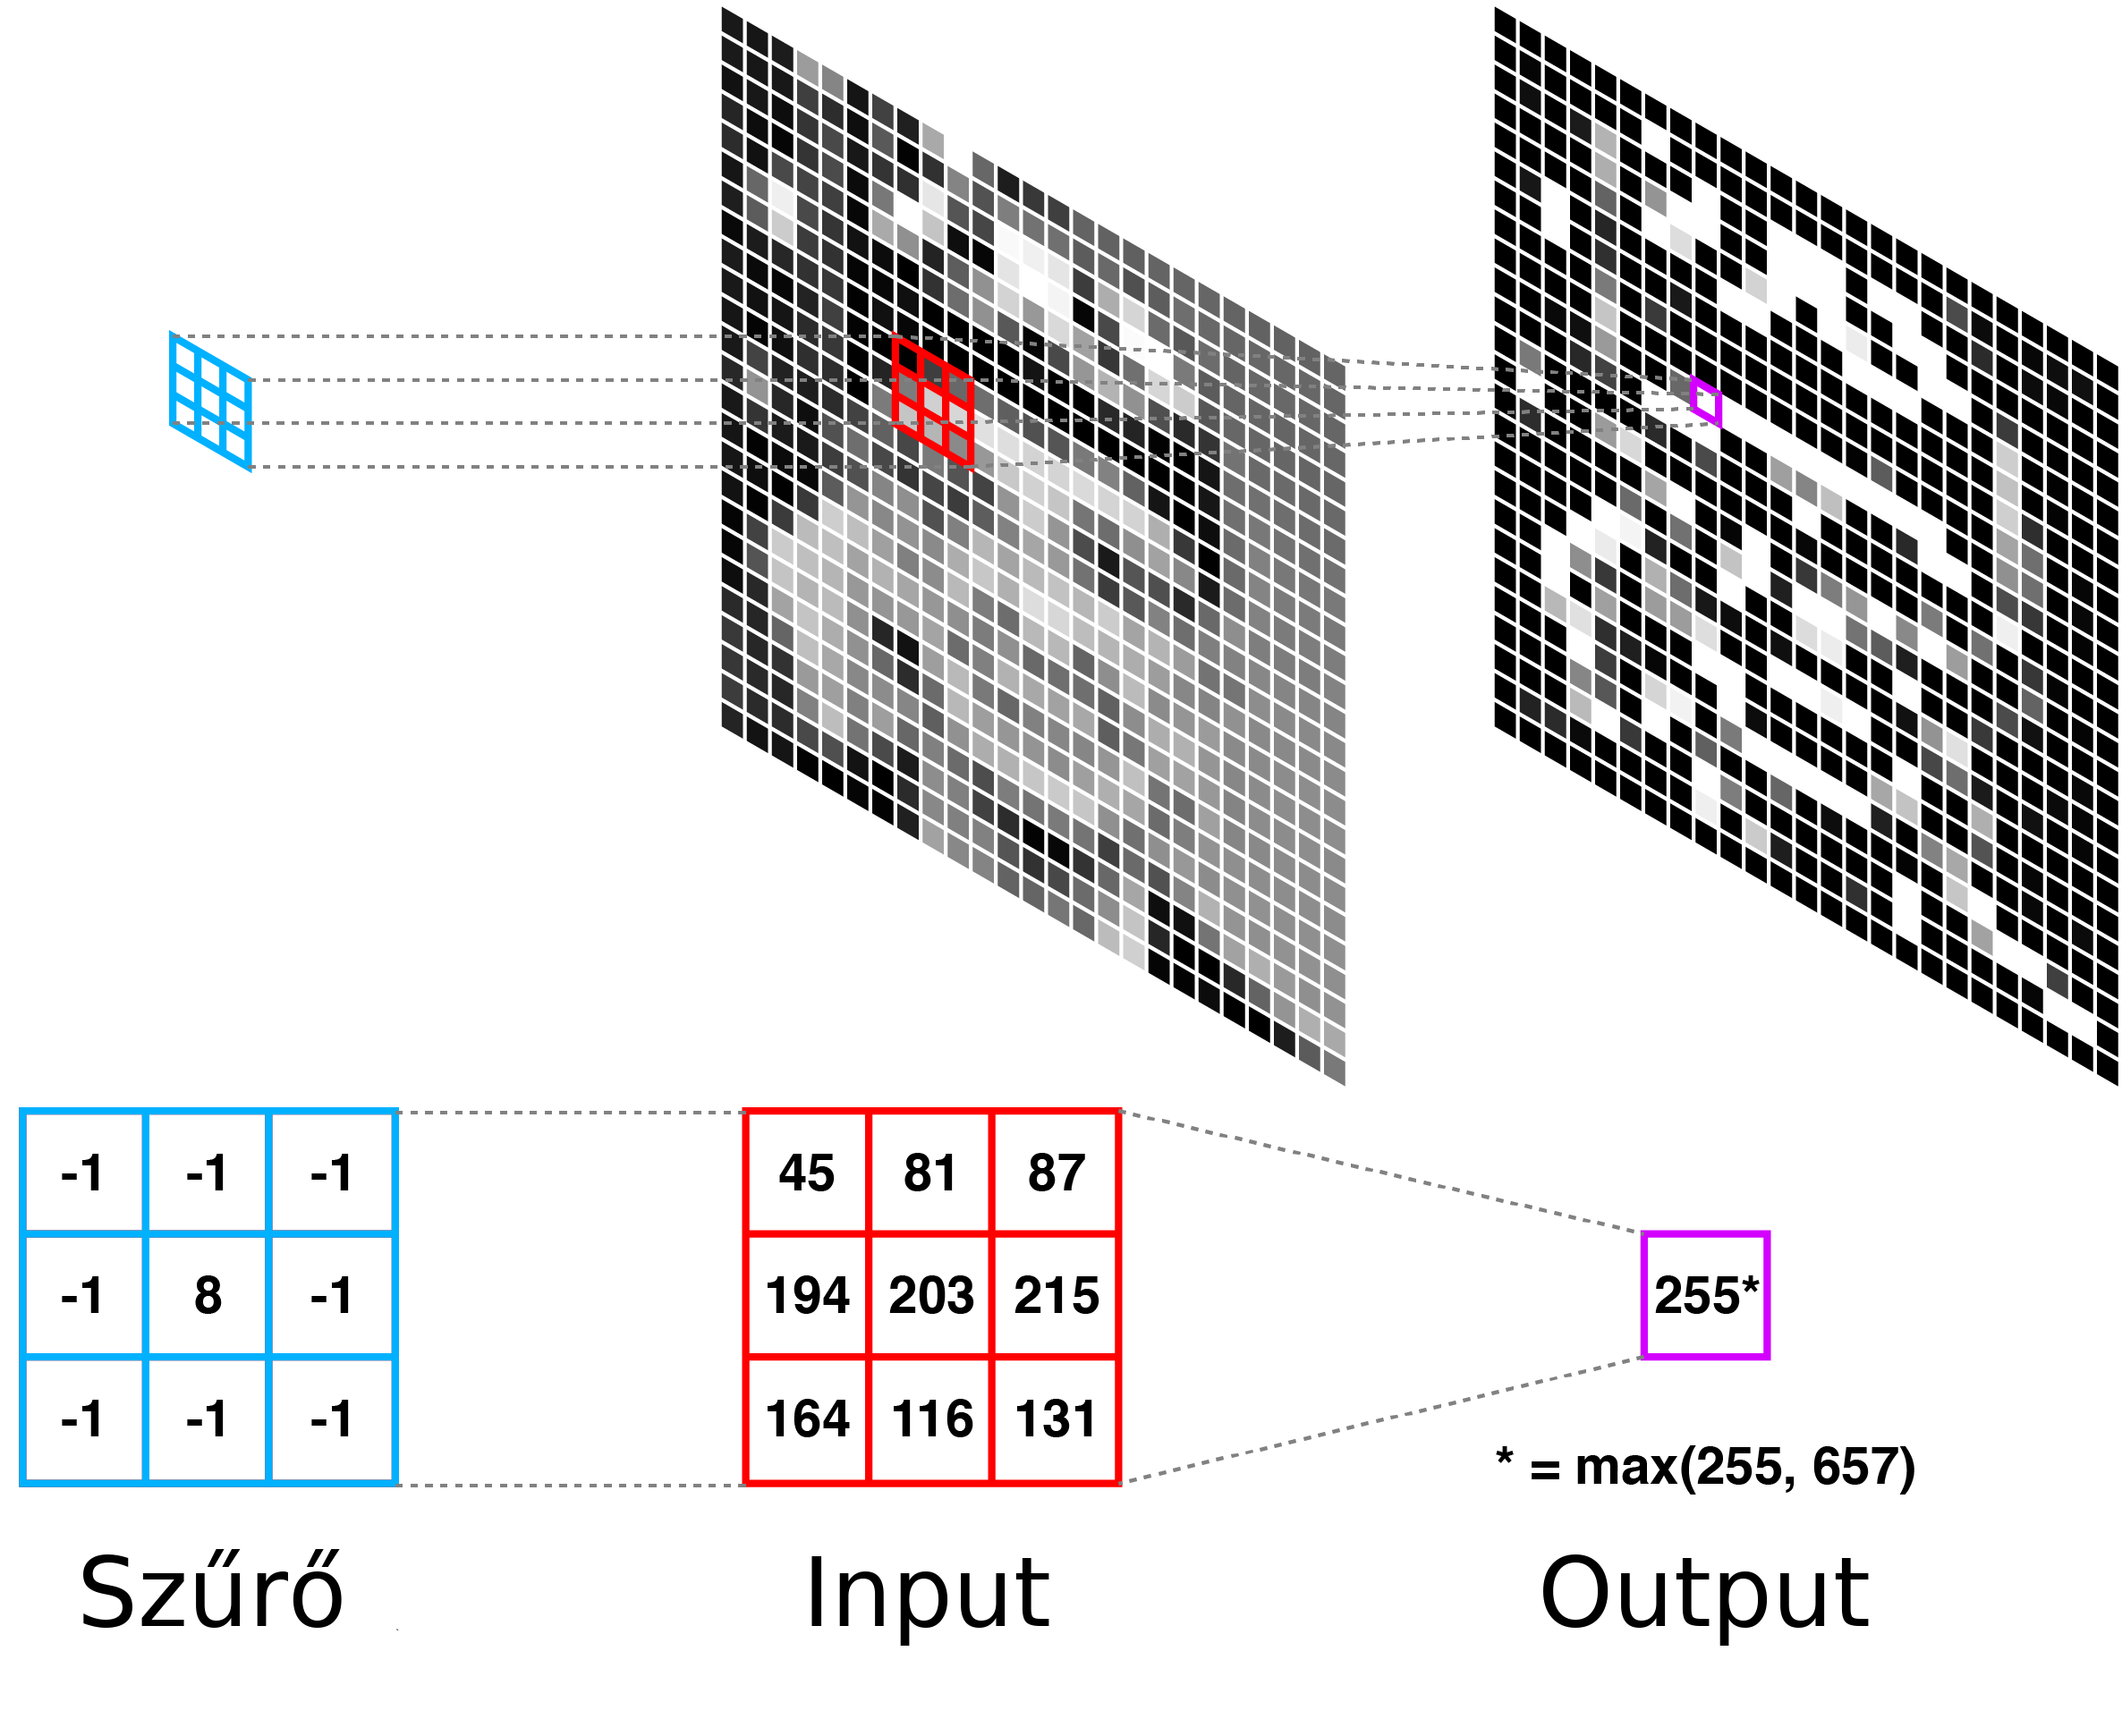
\includegraphics[height=7cm, width=7cm, keepaspectratio]{images/dl_4.png}
\end{center}
\end{column}
\end{columns}
\end{frame}

\begin{frame}{Konvolúció több dimenzióban}
\begin{columns}
\begin{column}{.5\textwidth}
A konvolúció általánosítható több dimenzióra is. A gyakorlatban 3D konvolúció megy végbe a neurális hálózatokban, \textbf{hiszen a színes képek 3D mátrixokban tárolódnak el}, ahol az egyes dimenziók a \emph{magasság, hosszúság és csatorna}. A csatorna három elemű és az R,G,B értékeket kódolja.\par\smallskip
A konvolúció tetszőleges dimenzióra általánosítható művelet.
\end{column}
\begin{column}{.5\textwidth}
\begin{center}
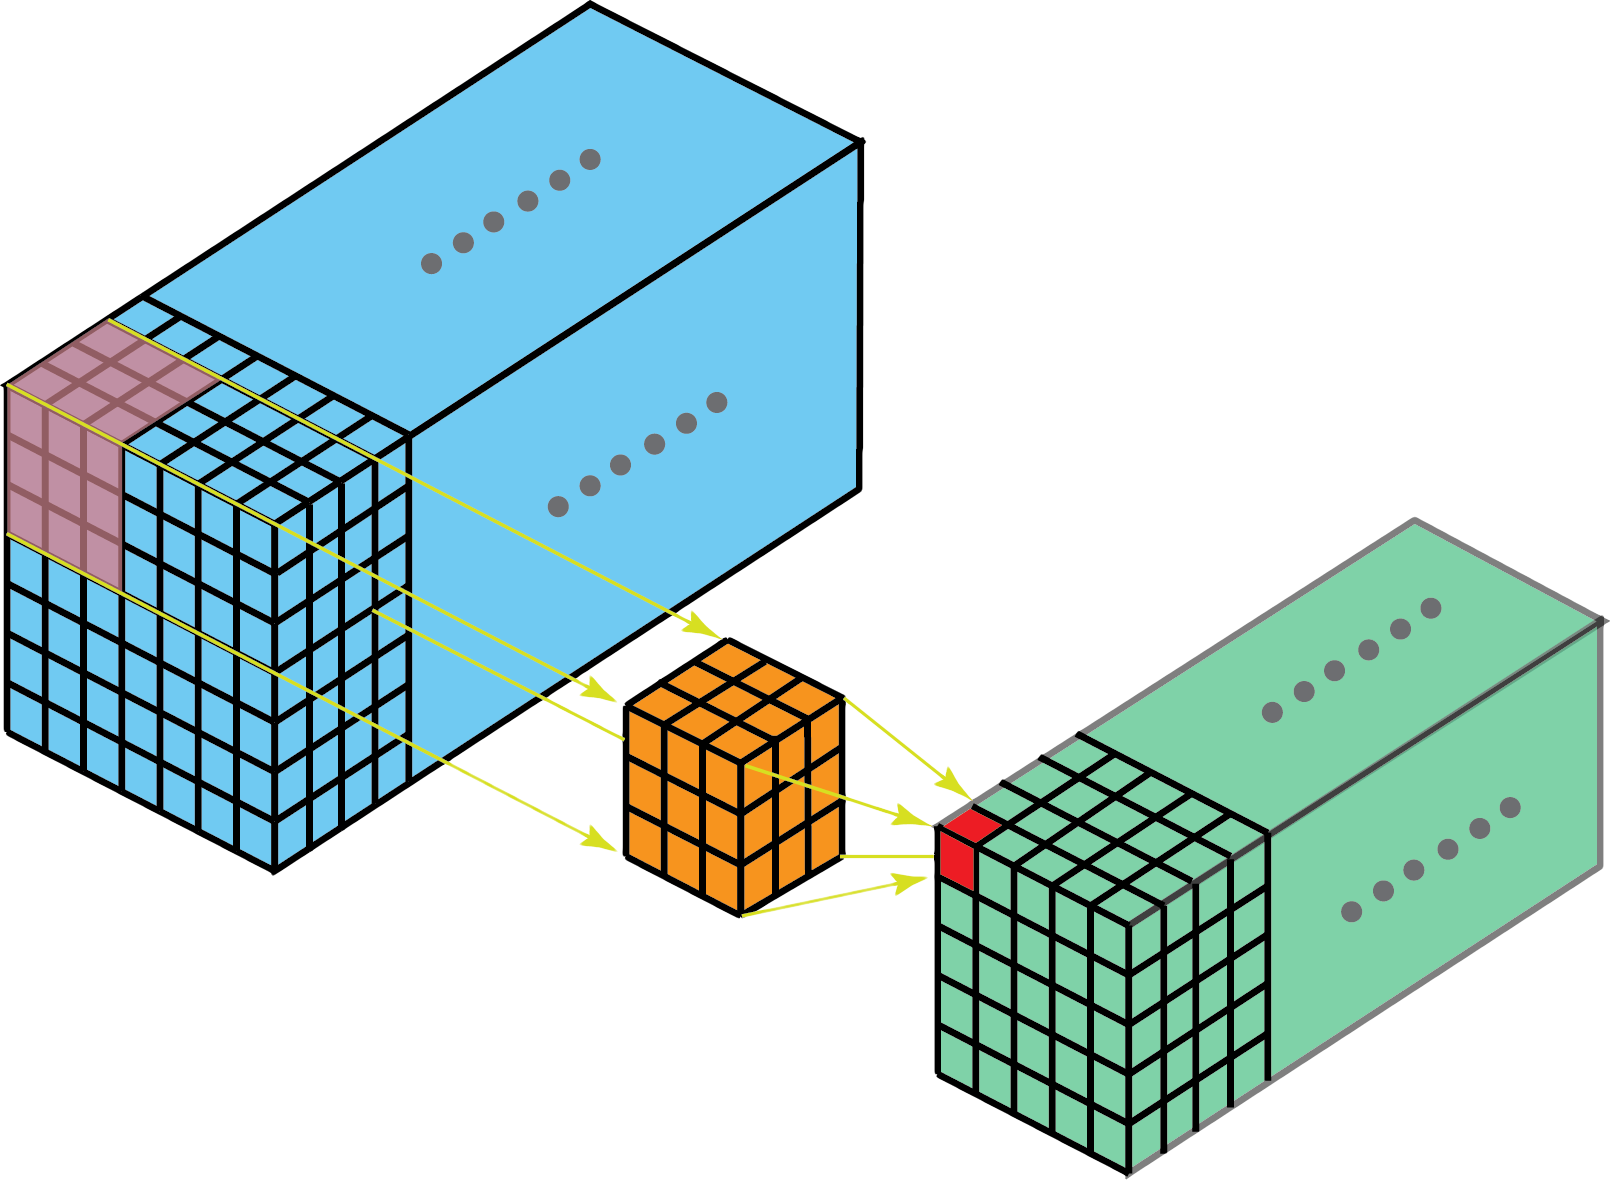
\includegraphics[height=7cm, width=7cm, keepaspectratio]{images/dl_5.png}
\end{center}
\end{column}
\end{columns}
\end{frame}

\begin{frame}{Pooling réteg}
\begin{columns}
\begin{column}{.5\textwidth}
A pooling vagy lazítás egy almintázási művelet, ami csökkenti a \textbf{bemenet térbeli dimenzióit}, miközben a fontos információt megtartja. A konvolúciós hálózatokban gyakran használatos a számítási igény csökkentésére, túltanulás elkerülésére és a hálózat segítésére abban, hogy fontos mintázatokat tanuljon meg.\par\smallskip
\begin{block}{Pooling neuron}
A vele kapcsolatban álló \textbf{neuronok output értékeit aggregálja valamilyen függvény szerint}. Leggyakrabban ez az \textbf{átlagolás} vagy a \textbf{maximum} kiválasztás.
\end{block}
\end{column}
\begin{column}{.5\textwidth}
\begin{center}
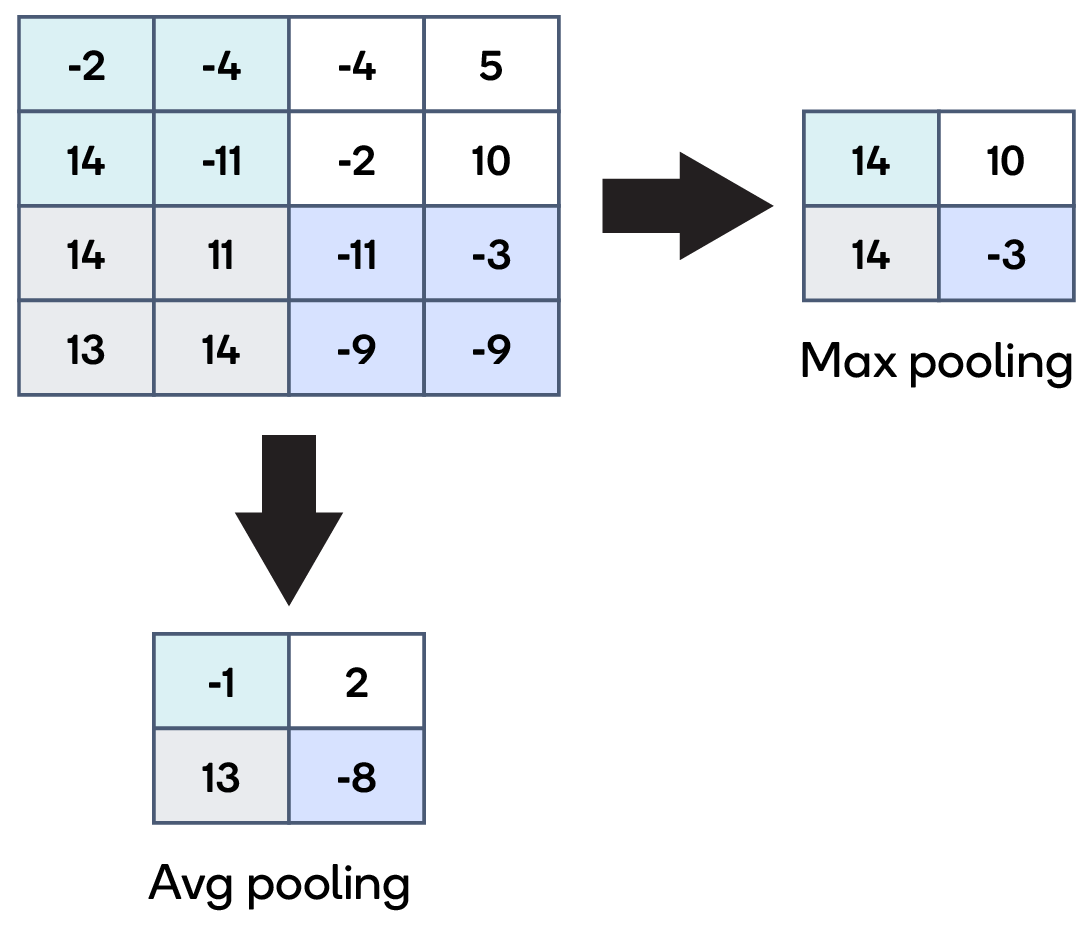
\includegraphics[height=5cm, width=7cm, keepaspectratio]{images/dl_6.png}
\end{center}
$\frac{1}{4}(-2 -4 +14 -11)=-1$\par\smallskip
$max\{-2, -4, 14, -11\}=14$
\end{column}
\end{columns}
\end{frame}

\begin{frame}{Teljes konvolúciós architektúra}
\begin{center}
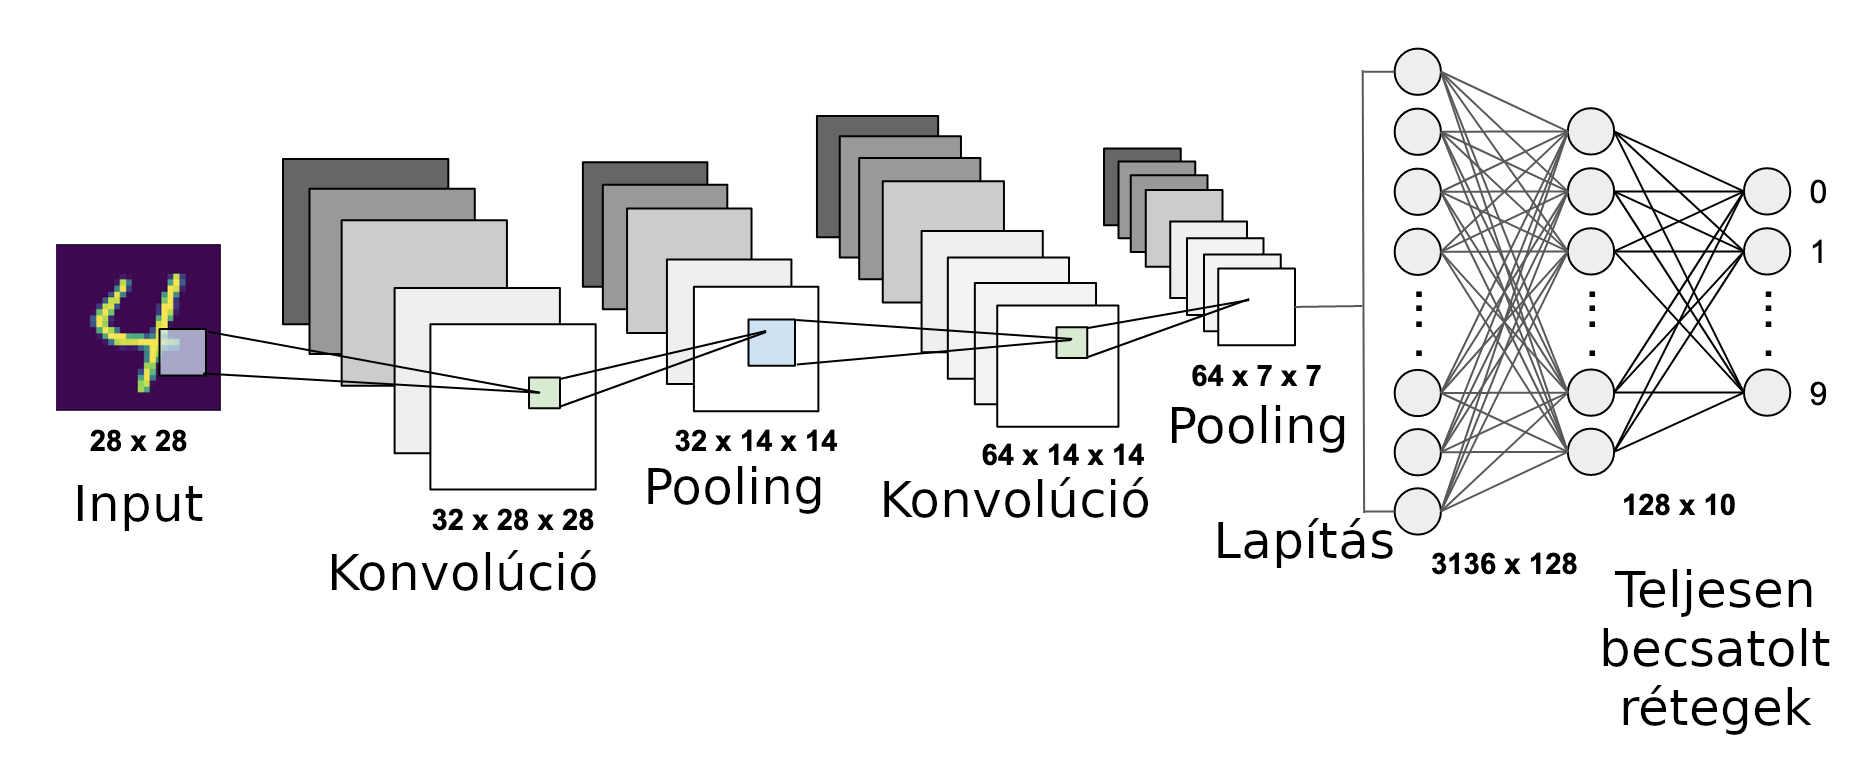
\includegraphics[height=7cm, width=14cm, keepaspectratio]{images/dl_7.png}
\end{center}
\end{frame}

\section{Önkódoló architektúrák}

\begin{frame}
\tableofcontents[currentsection]
\end{frame}

\begin{frame}{Önkódoló architektúra}
\begin{columns}
\begin{column}{.5\textwidth}
Az önkódoló architektúrák feladata megismerni \textbf{az inputnak egy tömörített reprezentációját}. Mivel nincs szükség címkére, az önkódoló egy \textbf{felügyelet nélküli} tanítási módszernek tekinthető. Viszont az \textbf{output az inputnak egy rekonstrukciója}, ezért tekinthető egy \textbf{önfelügyelt} tanítási módszernek is.
\only<1>{\begin{block}{Kódoló}
A hálózat azon része, amelyik az inputot egy csökkentett méretű látens dimenzióba tömöríti az inputot. Egy $h=f(x)$ kódoló függvénnyel reprezentálható.
\end{block}}
\only<2>{\begin{block}{Látens tér}
A hálózat azon része, amelyik tartalmazza az input csökkentett dimenziószámú reprezentációját.
\end{block}}
\only<3>{\begin{block}{Dekódoló}
A hálózat azon része, amelyik a látens reprezentációt rekonstruálja. Struktúrája hasonló a kódolóéhoz. Egy $r=g(h)$ függvénnyel jelölhető.
\end{block}}
\end{column}
\begin{column}{.5\textwidth}
\begin{center}
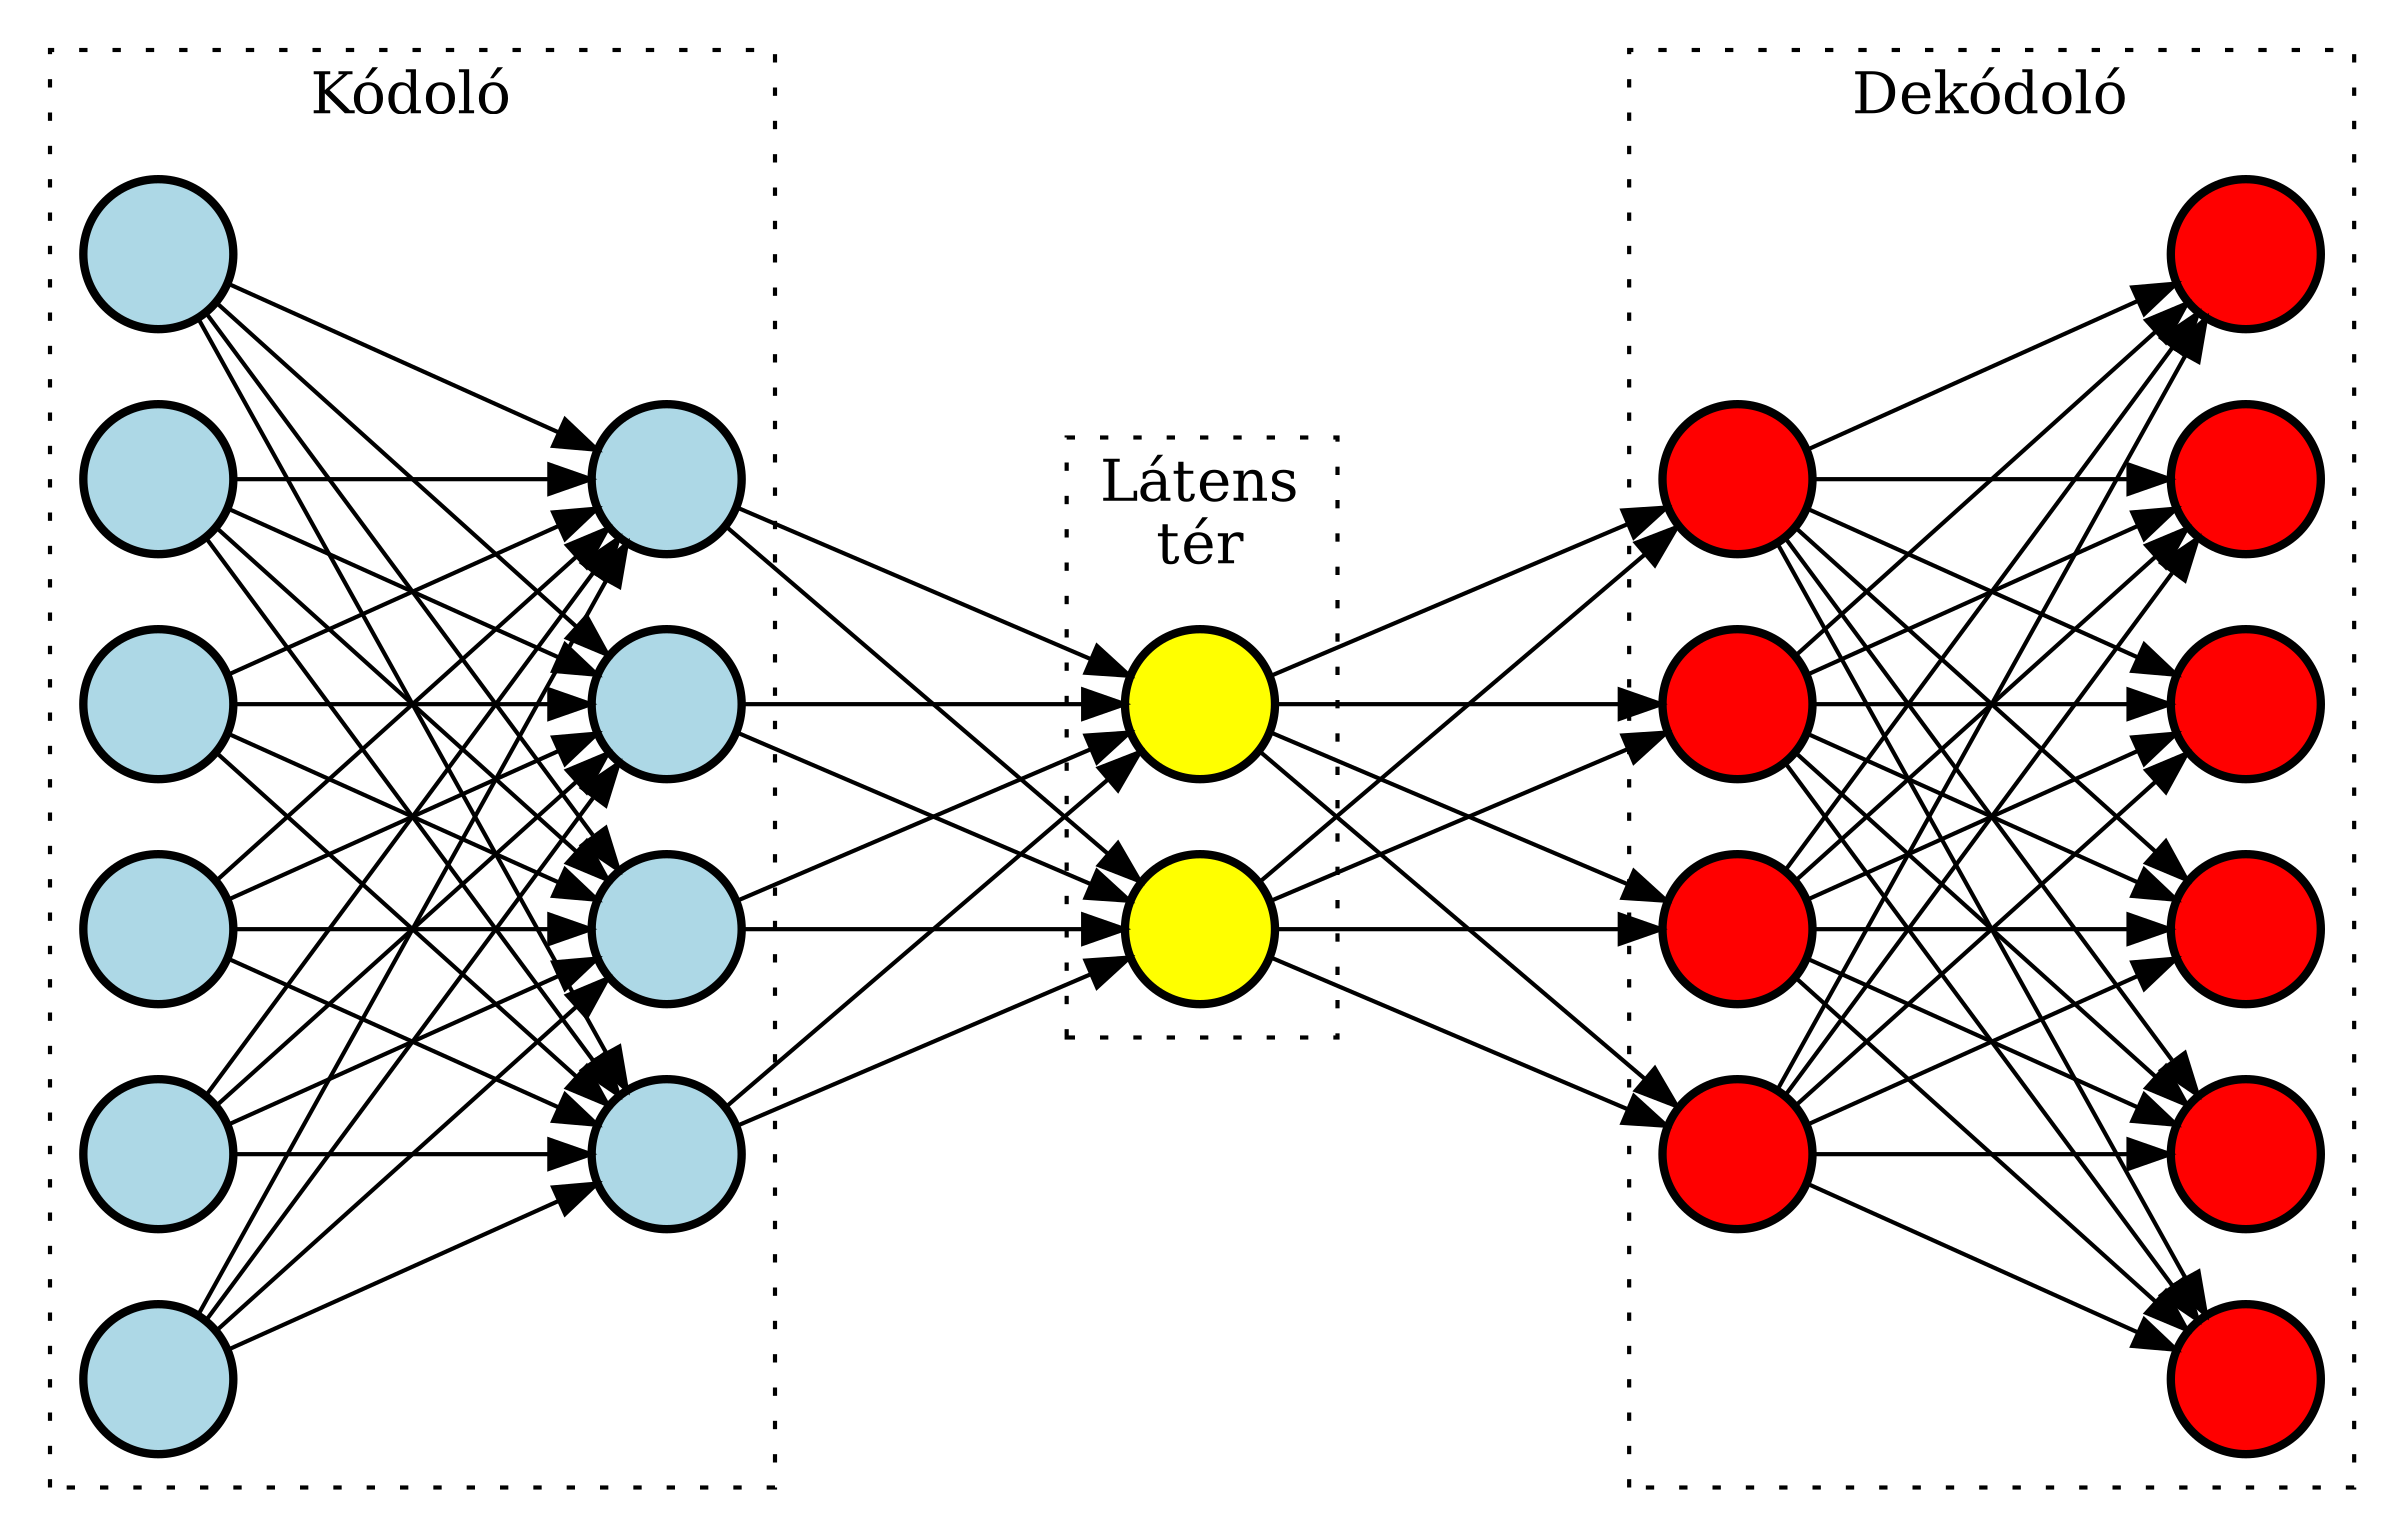
\includegraphics[height=7cm, width=7cm, keepaspectratio]{graphs/dl_4.png}
\end{center}
\end{column}
\end{columns}
\end{frame}

\begin{frame}{Konvolúciós önkódolók}
A konvolúciós önkódoló architektúrák kombinálják az önkódolók eredeti koncepcióját a konvolúciós rétegekkel. Az architektúra jól illeszkedik képfeldolgozó feladatokra, mint zajszűrés, tömörítés és mintázatok elsajátítása. Ebben az esetben \textbf{a hálózat inputja és outputja is egy kép}.
\begin{center}
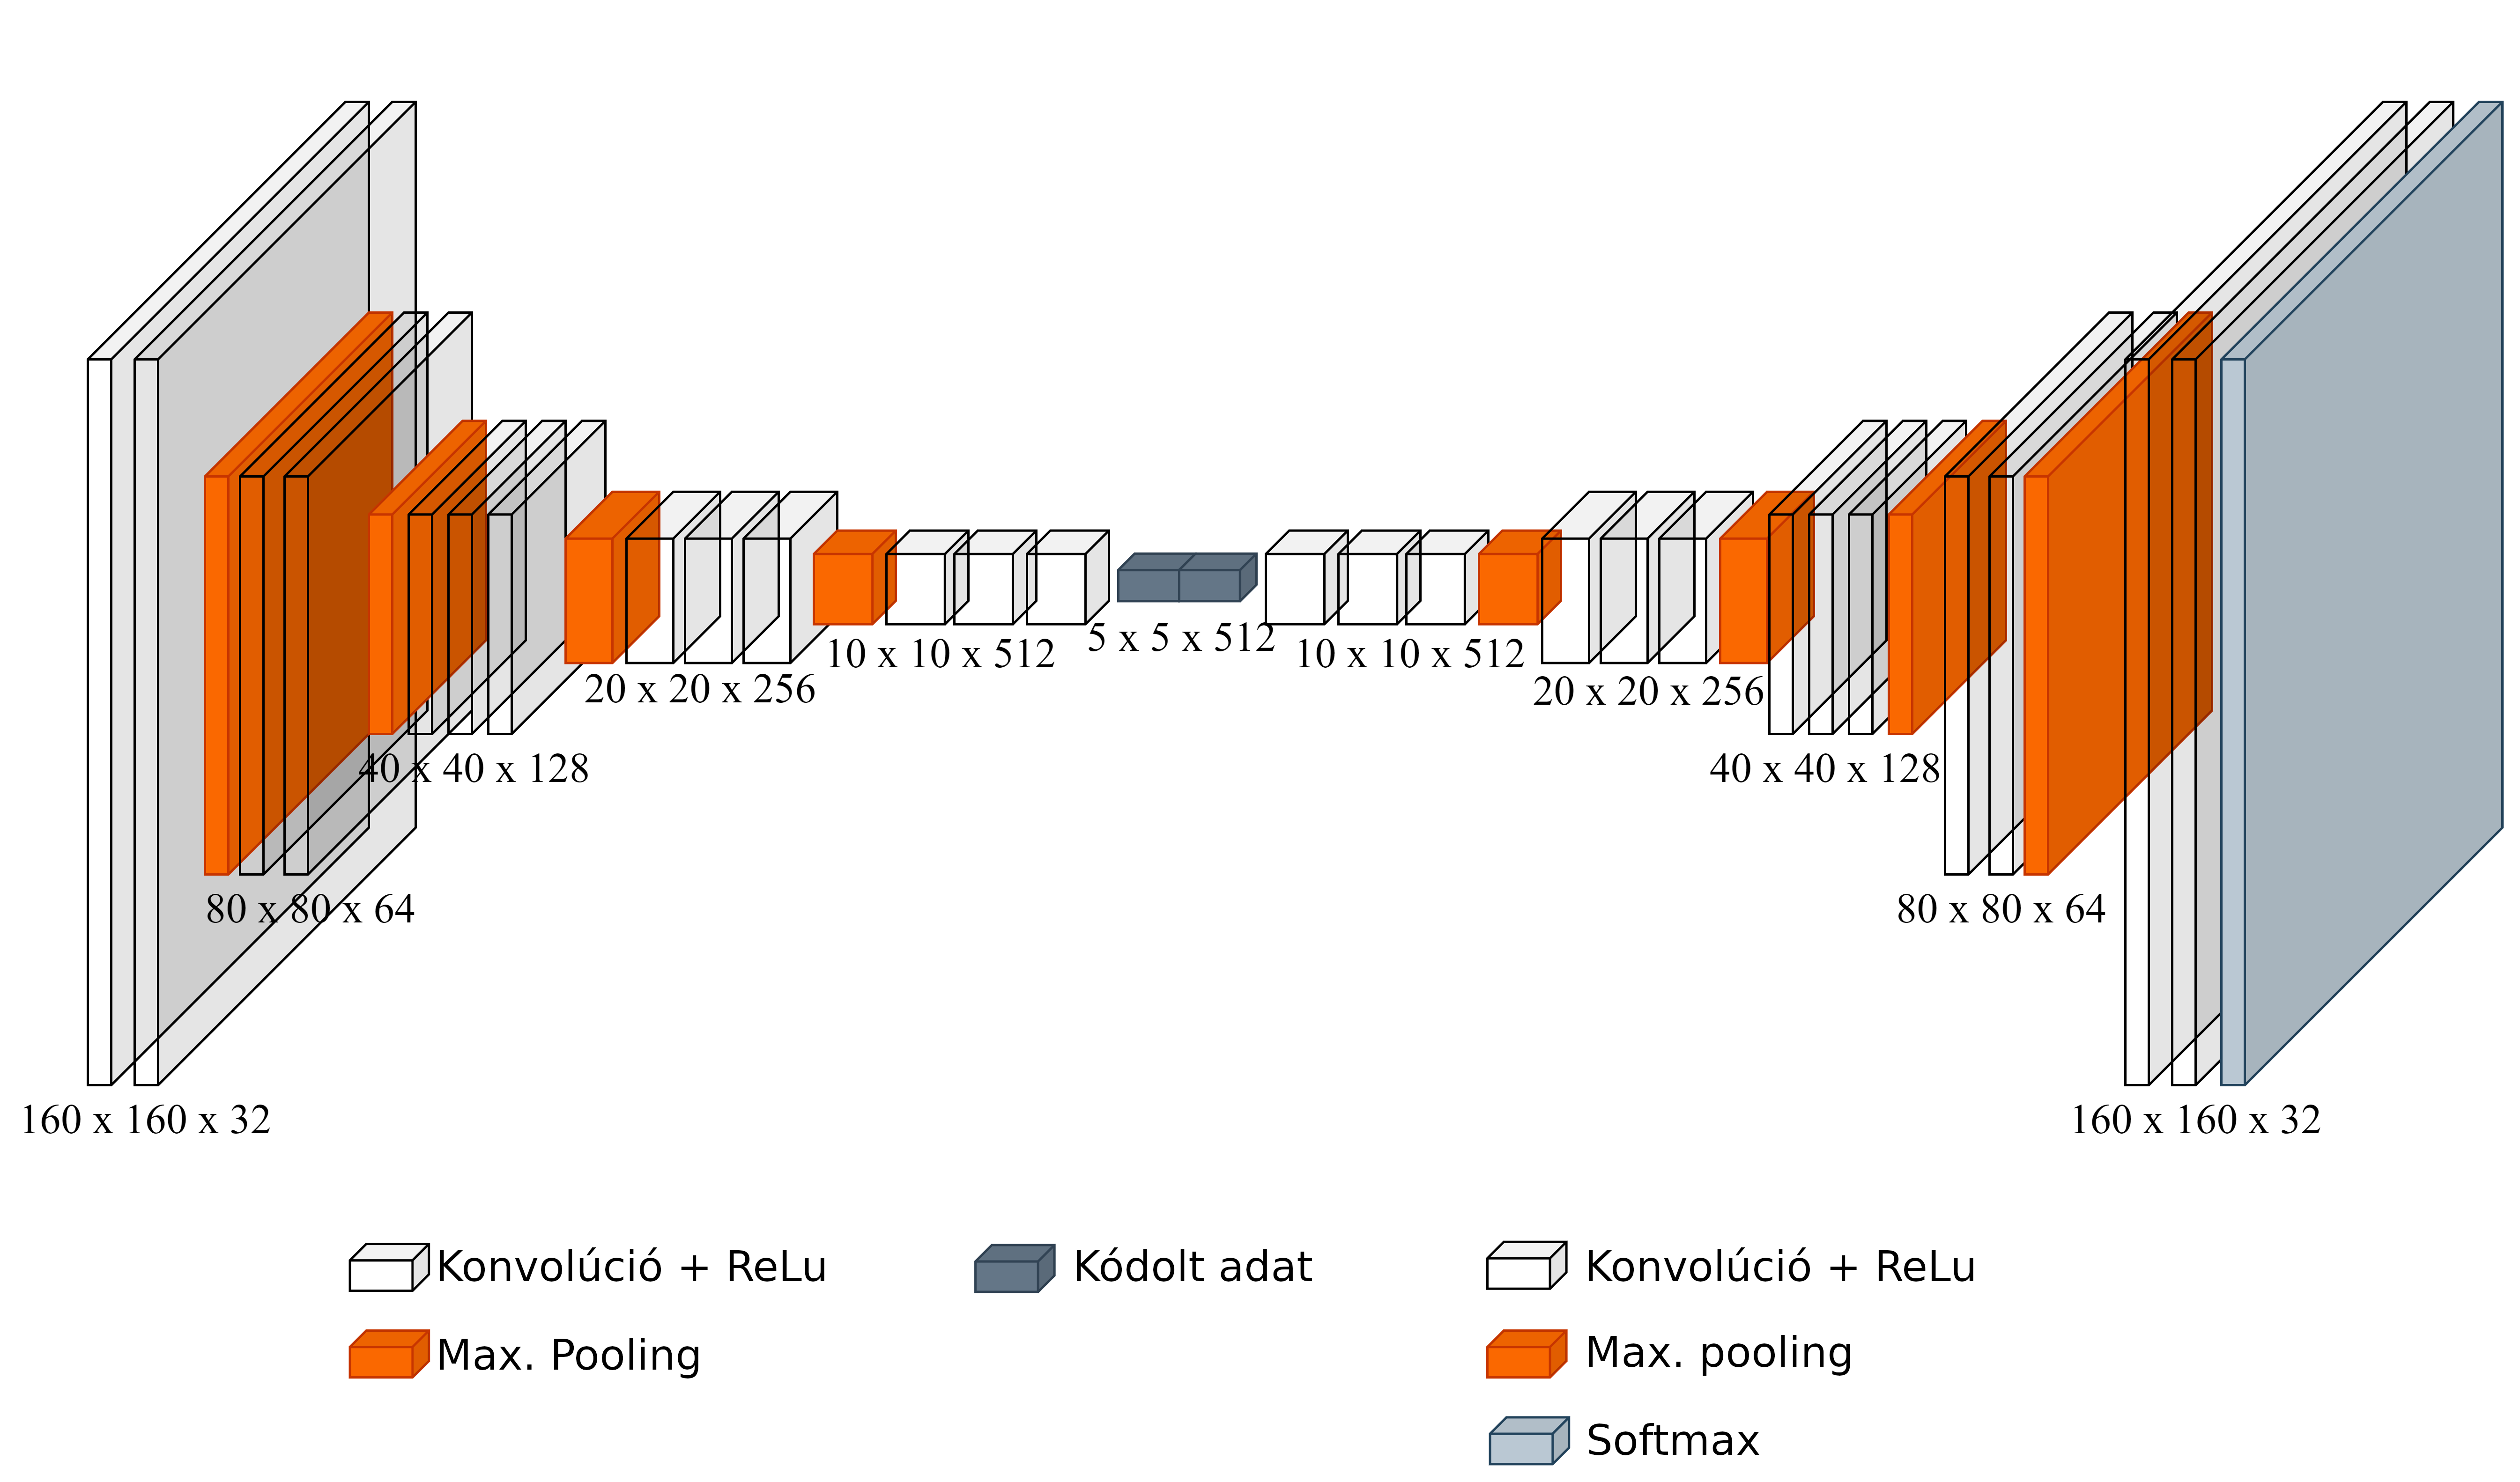
\includegraphics[height=7cm, width=9cm, keepaspectratio]{images/dl_9.png}
\end{center}
\end{frame}

\begin{frame}{Zajszűrő önkódolók}
A \textbf{kódoló} zajos adatot fogad inputként, és átalakítja egy alacsonyabb dimenziós reprezentációvá. Ennek a reprezentációnak a feladata megragadni az input belső struktúráját és fontos mintázatait.\\
A \textbf{dekódoló} a kódolt reprezentációt fogadja inputként és a célja, hogy rekonstruálja az eredeti, zajmentes adatot.
\begin{center}
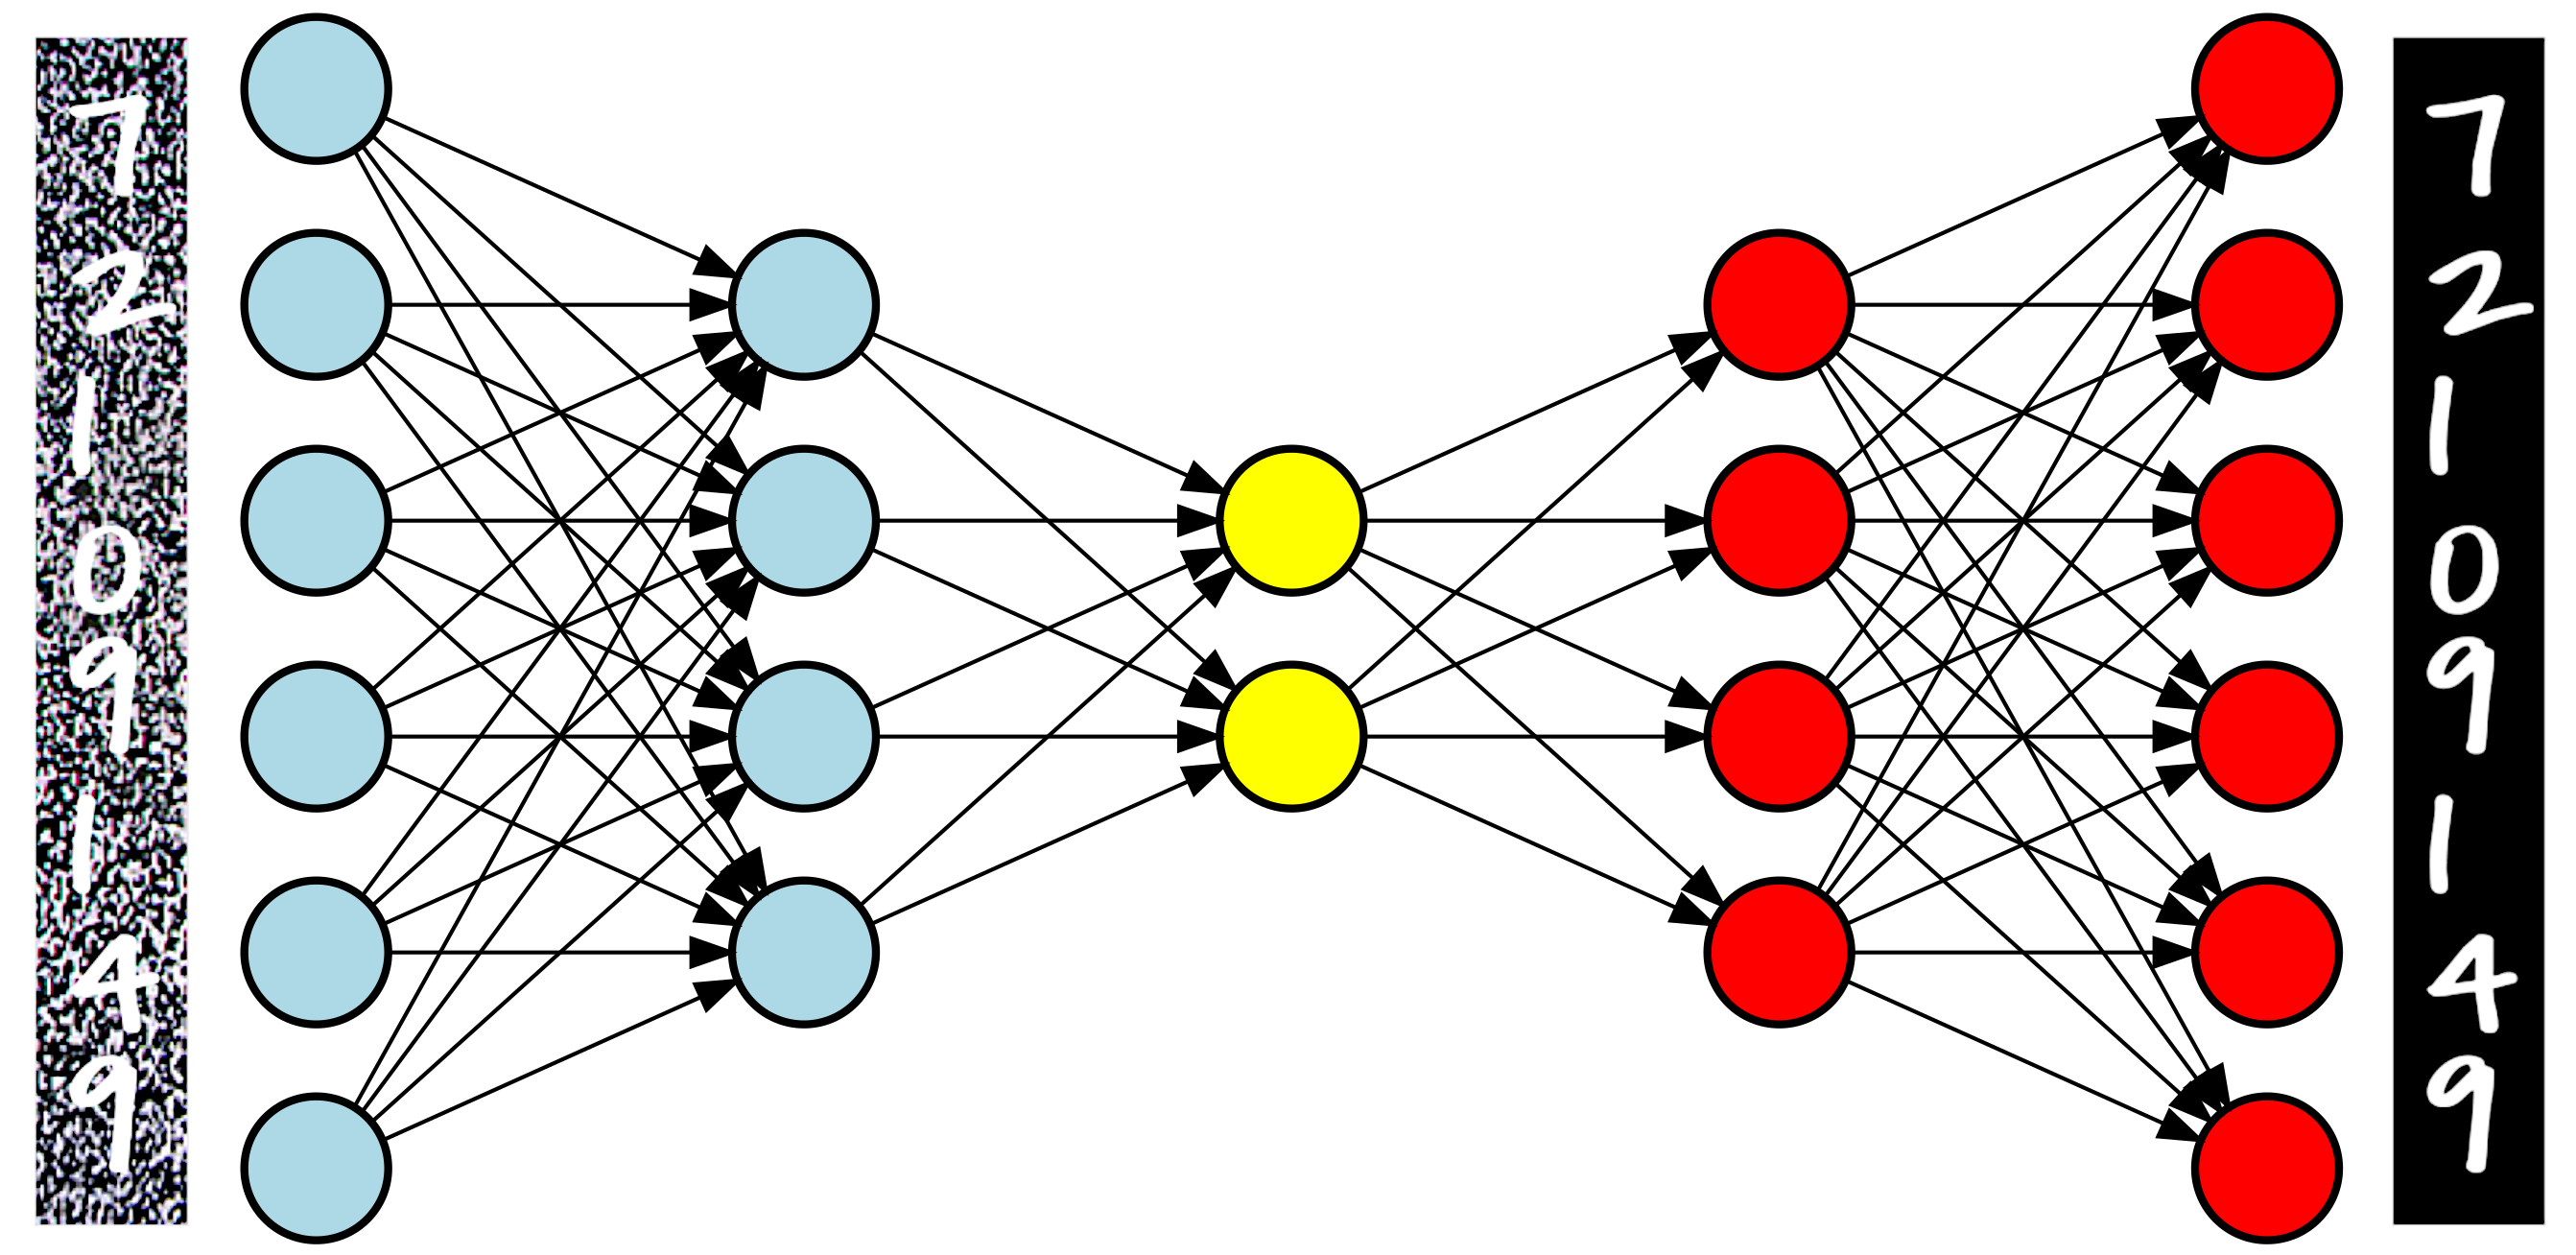
\includegraphics[width=9cm, keepaspectratio]{images/dl_10.png}
\end{center}
\end{frame}

\begin{frame}{Variációs önkódolók}
\begin{columns}
\begin{column}{.7\textwidth}
A variációs önkódolók az önkódoló mélytanuló architektúrák \textbf{probabilisztikus, generatív} változatai. A hagyományos önkódolóktól eltérően ahelyett, hogy egy input adat-szám leképező függvényt tanulnának meg, \textbf{az adathalmaznak a valószínűségeloszlását tanulják meg reprezentálni}.\par\smallskip
A kódoló egy $P(z|x)$ valószínűségeloszlásra képezi rá az input adatot. Ezt az eloszlást $\mu$ várható érték és $\sigma$ szóródás határozza meg.\par\smallskip
A dekódoló mintát vesz a látens tér eloszlásából: $z = \mu + \sigma \cdot \varepsilon$, ahol $\varepsilon$ a zaj és a $P(x'|z)$ valószínűségeloszlás alapján állítja elő az outputot.\par\smallskip
Mivel a variációs önkódolók megismerik az adatok alacsony szintű eloszlását, lehetséges új mintaadatokat generálni az eloszlásokból való mintavétellel. 
\end{column}
\begin{column}{.3\textwidth}
\begin{center}
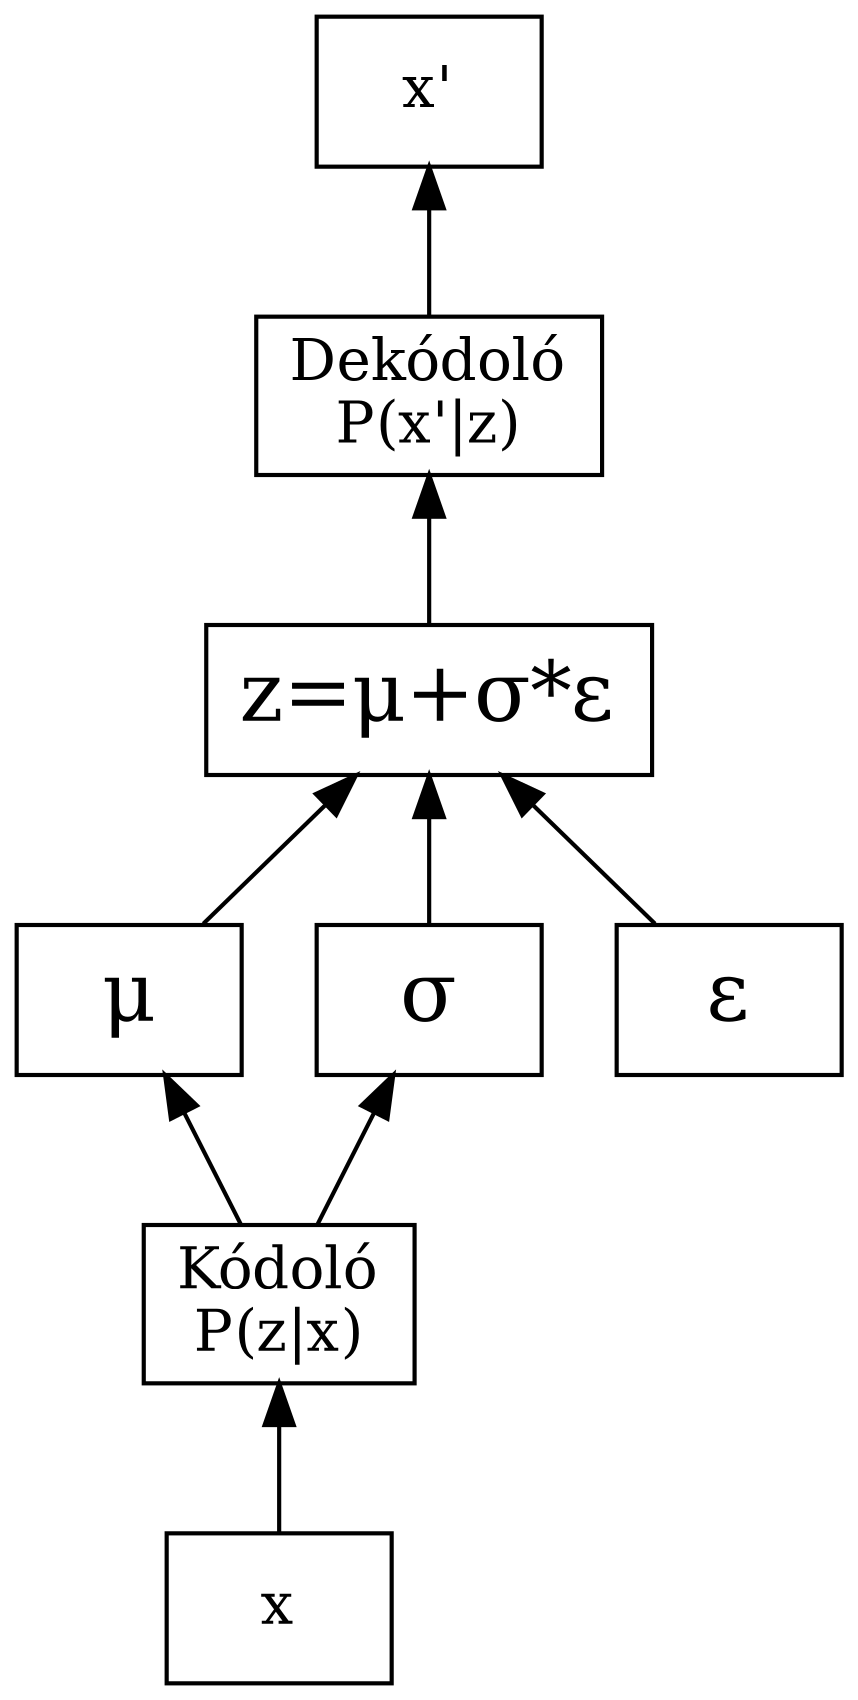
\includegraphics[height=7cm, keepaspectratio]{graphs/dl_6.png}
\end{center}
\end{column}
\end{columns}
\end{frame}

\begin{frame}{Szegmentációs önkódolók}
Az önkódoló architektúrák használhatóak képszegmentálásra is. Ebben az esetben a hálózat feladata \textbf{felosztani a képet különálló régiókra szemantikai értelmezés szerint}.\par\smallskip Szegmentáció esetén a cél egy különböző képet előállítani mint az eredeti, amelynek az értelmezése is különbözik az eredetiétől. Ebben az esetben egy képből lesz egy szemantikai maszk, amely minden pixelről eldönti, melyik osztályba tartozik. 
\begin{center}
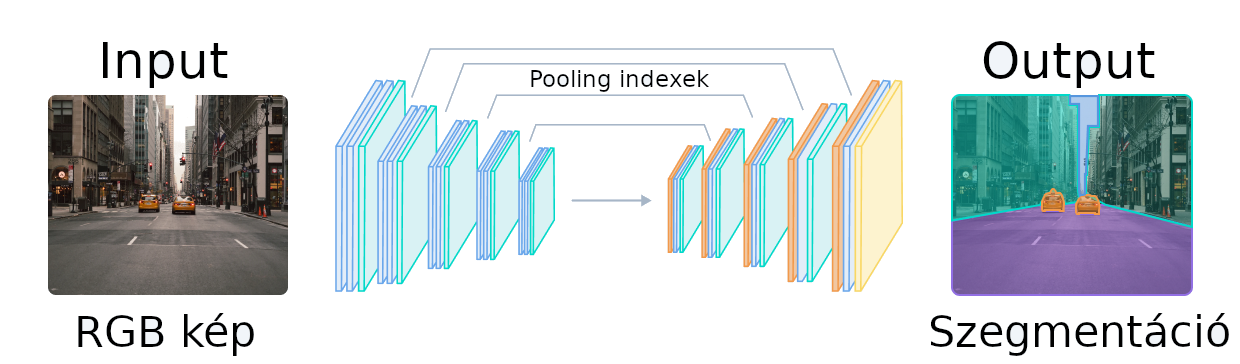
\includegraphics[width=12cm, keepaspectratio]{images/dl_11.png}
\end{center} 
\end{frame}

\end{document}










